% Options for packages loaded elsewhere
\PassOptionsToPackage{unicode}{hyperref}
\PassOptionsToPackage{hyphens}{url}
\PassOptionsToPackage{dvipsnames,svgnames,x11names}{xcolor}
%
\documentclass[
  12pt,
]{book}
\usepackage{amsmath,amssymb}
\usepackage{lmodern}
\usepackage{setspace}
\usepackage{iftex}
\ifPDFTeX
  \usepackage[T1]{fontenc}
  \usepackage[utf8]{inputenc}
  \usepackage{textcomp} % provide euro and other symbols
\else % if luatex or xetex
  \usepackage{unicode-math}
  \defaultfontfeatures{Scale=MatchLowercase}
  \defaultfontfeatures[\rmfamily]{Ligatures=TeX,Scale=1}
\fi
% Use upquote if available, for straight quotes in verbatim environments
\IfFileExists{upquote.sty}{\usepackage{upquote}}{}
\IfFileExists{microtype.sty}{% use microtype if available
  \usepackage[]{microtype}
  \UseMicrotypeSet[protrusion]{basicmath} % disable protrusion for tt fonts
}{}
\makeatletter
\@ifundefined{KOMAClassName}{% if non-KOMA class
  \IfFileExists{parskip.sty}{%
    \usepackage{parskip}
  }{% else
    \setlength{\parindent}{0pt}
    \setlength{\parskip}{6pt plus 2pt minus 1pt}}
}{% if KOMA class
  \KOMAoptions{parskip=half}}
\makeatother
\usepackage{xcolor}
\IfFileExists{xurl.sty}{\usepackage{xurl}}{} % add URL line breaks if available
\IfFileExists{bookmark.sty}{\usepackage{bookmark}}{\usepackage{hyperref}}
\hypersetup{
  pdftitle={Rで学ぶ『完全独習 統計学入門』},
  pdfauthor={Sampo Suzuki, CC 4.0 BY-NC-SA},
  colorlinks=true,
  linkcolor={Maroon},
  filecolor={Maroon},
  citecolor={Blue},
  urlcolor={Blue},
  pdfcreator={LaTeX via pandoc}}
\urlstyle{same} % disable monospaced font for URLs
\usepackage{color}
\usepackage{fancyvrb}
\newcommand{\VerbBar}{|}
\newcommand{\VERB}{\Verb[commandchars=\\\{\}]}
\DefineVerbatimEnvironment{Highlighting}{Verbatim}{commandchars=\\\{\}}
% Add ',fontsize=\small' for more characters per line
\usepackage{framed}
\definecolor{shadecolor}{RGB}{248,248,248}
\newenvironment{Shaded}{\begin{snugshade}}{\end{snugshade}}
\newcommand{\AlertTok}[1]{\textcolor[rgb]{0.94,0.16,0.16}{#1}}
\newcommand{\AnnotationTok}[1]{\textcolor[rgb]{0.56,0.35,0.01}{\textbf{\textit{#1}}}}
\newcommand{\AttributeTok}[1]{\textcolor[rgb]{0.77,0.63,0.00}{#1}}
\newcommand{\BaseNTok}[1]{\textcolor[rgb]{0.00,0.00,0.81}{#1}}
\newcommand{\BuiltInTok}[1]{#1}
\newcommand{\CharTok}[1]{\textcolor[rgb]{0.31,0.60,0.02}{#1}}
\newcommand{\CommentTok}[1]{\textcolor[rgb]{0.56,0.35,0.01}{\textit{#1}}}
\newcommand{\CommentVarTok}[1]{\textcolor[rgb]{0.56,0.35,0.01}{\textbf{\textit{#1}}}}
\newcommand{\ConstantTok}[1]{\textcolor[rgb]{0.00,0.00,0.00}{#1}}
\newcommand{\ControlFlowTok}[1]{\textcolor[rgb]{0.13,0.29,0.53}{\textbf{#1}}}
\newcommand{\DataTypeTok}[1]{\textcolor[rgb]{0.13,0.29,0.53}{#1}}
\newcommand{\DecValTok}[1]{\textcolor[rgb]{0.00,0.00,0.81}{#1}}
\newcommand{\DocumentationTok}[1]{\textcolor[rgb]{0.56,0.35,0.01}{\textbf{\textit{#1}}}}
\newcommand{\ErrorTok}[1]{\textcolor[rgb]{0.64,0.00,0.00}{\textbf{#1}}}
\newcommand{\ExtensionTok}[1]{#1}
\newcommand{\FloatTok}[1]{\textcolor[rgb]{0.00,0.00,0.81}{#1}}
\newcommand{\FunctionTok}[1]{\textcolor[rgb]{0.00,0.00,0.00}{#1}}
\newcommand{\ImportTok}[1]{#1}
\newcommand{\InformationTok}[1]{\textcolor[rgb]{0.56,0.35,0.01}{\textbf{\textit{#1}}}}
\newcommand{\KeywordTok}[1]{\textcolor[rgb]{0.13,0.29,0.53}{\textbf{#1}}}
\newcommand{\NormalTok}[1]{#1}
\newcommand{\OperatorTok}[1]{\textcolor[rgb]{0.81,0.36,0.00}{\textbf{#1}}}
\newcommand{\OtherTok}[1]{\textcolor[rgb]{0.56,0.35,0.01}{#1}}
\newcommand{\PreprocessorTok}[1]{\textcolor[rgb]{0.56,0.35,0.01}{\textit{#1}}}
\newcommand{\RegionMarkerTok}[1]{#1}
\newcommand{\SpecialCharTok}[1]{\textcolor[rgb]{0.00,0.00,0.00}{#1}}
\newcommand{\SpecialStringTok}[1]{\textcolor[rgb]{0.31,0.60,0.02}{#1}}
\newcommand{\StringTok}[1]{\textcolor[rgb]{0.31,0.60,0.02}{#1}}
\newcommand{\VariableTok}[1]{\textcolor[rgb]{0.00,0.00,0.00}{#1}}
\newcommand{\VerbatimStringTok}[1]{\textcolor[rgb]{0.31,0.60,0.02}{#1}}
\newcommand{\WarningTok}[1]{\textcolor[rgb]{0.56,0.35,0.01}{\textbf{\textit{#1}}}}
\usepackage{longtable,booktabs,array}
\usepackage{calc} % for calculating minipage widths
% Correct order of tables after \paragraph or \subparagraph
\usepackage{etoolbox}
\makeatletter
\patchcmd\longtable{\par}{\if@noskipsec\mbox{}\fi\par}{}{}
\makeatother
% Allow footnotes in longtable head/foot
\IfFileExists{footnotehyper.sty}{\usepackage{footnotehyper}}{\usepackage{footnote}}
\makesavenoteenv{longtable}
% Make links footnotes instead of hotlinks:
\DeclareRobustCommand{\href}[2]{#2\footnote{\url{#1}}}
\setlength{\emergencystretch}{3em} % prevent overfull lines
\providecommand{\tightlist}{%
  \setlength{\itemsep}{0pt}\setlength{\parskip}{0pt}}
\setcounter{secnumdepth}{5}
% --- 参考資料 ----------------------------------------------------------------
% https://github.com/Gedevan-Aleksizde/Japan.R2019/blob/master/latex/preamble.tex
% https://teastat.blogspot.com/2019/01/bookdown.html

% --- 未解決事項 --------------------------------------------------------------
% 1)knitr時に以下のワーニングが出る
%  警告メッセージ: 
% Package xeCJK Warning: Redefining CJKfamily `\CJKttdefault'
% (xeCJK)                (NotoSansCJKjp-Regular). 
% 
% 2) Bibliographyページを目次に表示できない
% 
% 3) 文頭一文字インデントを有効にできない
%    \usepackage{indentfirst}   # インストールできない
% 

% --- Packages ----------------------------------------------------------------
% 日本語とtufte, kableExtraを使うために必要なTeXパッケージ指定
%  A4 210mm x 297mm
%   \usepackage[a4paper, total={6.5in, 9.5in}]{geometry}
%   \usepackage{indentfirst}   # tinytexのリポジトリには存在しない?

\usepackage[a4paper, total={160mm, 247mm}, left=25mm, top=25mm]{geometry}
% \usepackage[pdfbox,tombo]{gentombow}  % トンボを設定する場合は有効にする
\usepackage{ifthen}                     % 条件分岐用 \ifthenelse{条件}{T}{F}
\usepackage{booktabs}                   % ここからkableExtra用パッケージ
\usepackage{longtable}                  % 
\usepackage{array}                      % 
\usepackage{multirow}                   % 
\usepackage{wrapfig}                    % 
\usepackage{float}                      % 
\usepackage{colortbl}                   % 
\usepackage{pdflscape}                  % 
\usepackage{tabu}                       % 
\usepackage{threeparttable}             % 
\usepackage{threeparttablex}            % 
\usepackage[normalem]{ulem}             % 
\usepackage{inputenc}                   % 
\usepackage{makecell}                   % 
\usepackage{xcolor}                     % ここまでkableExtra用
\usepackage{amsmath}                    % 
\usepackage{fontawesome5}               % fontawesomeを使うために必要
\usepackage{subfig}
\usepackage{xeCJK}                      % 以下、日本語フォント用に必要
\usepackage{zxjatype}
\usepackage[noto]{zxjafont}             % Linux環境ではこちを指定
% \usepackage[haranoaji]{zxjafont}      % Windows環境ではこちらを指定する
% \usepackage[nopreset]{zxjafont}         % メイン設定を何も行わない場合
\usepackage{pxrubrica}                  % ルビ用
\usepackage{hyperref}                   % ハイパーリンク用必要?

% --- Index ------------------------------------------------------------------
% https://texwiki.texjp.org/?%E7%B4%A2%E5%BC%95%E4%BD%9C%E6%88%90
\usepackage{makeidx}
\makeindex
% \usepackage{showidx}                  % 索引確認用(索引は作成されない)
% % 別名索引の定義はbefore_body.texにて
% --- 日本語索引 --------------------------------------------------------------
% 使い方がよくわからない(makeidxのようにはいかないので何か設定が必要か?)
% http://tug.ctan.org/info/mendex-doc/mendex.pdf
% \usepackage{mendex}
% \mendex

% --- Table of Contentes ------------------------------------------------------
% TOCにLOT(List of Tables), LOF(List of Figures), Bibliography, Indexを表示
\usepackage[nottoc]{tocbibind}

% --- Fonts -------------------------------------------------------------------
% フォントしては index.html でも可能(pandoc用オプションは index.htmlにて)
\setmonofont{Source Han Code JP}
\setCJKmonofont{Source Han Code JP}
% \setjamonofont{Source Han Code JP}
% \setmonofont{UDEV Gothic JPDOC}  % BIZ UD + JetBrais Mono
% \setCJKmonofont{UDEV Gothic JPDOC}

% ## 日本語フォントの扱いについてはzxjafontパッケージの解説を参照のこと
% # https://mirror.las.iastate.edu/tex-archive/language/japanese/zxjafont/zxjafont.pdf
% #
% ## Windows環境ではなぜかNotoフォントが認識されないので源ノシリーズベースの
% ## 原ノ味フォントかIPAexフォントを利用する(原ノ味はtlmgrでインストール可)
% # \usepackage[haranoaji]{zxjafont}
% # \usepackage[ipaex]{zxjafont}
% #
% ## Windows環境でNotoフォントを指定したい場合は以下のようにheader-includeで
% ## 個別に指定する(setCJKxxxfotnの指定は必要?)
% # \setmainfont{NotoSerifCJKjp-Regular.otf}[BoldFont=NotoSerifCJKjp-Bold.otf]
% # \setsansfont{NotoSansCJKjp-Regular.otf}[BoldFont=NotoSansCJKjp-Bold.otf]
% # \setmonofont{NotoSansMonoCJKjp-Regular.otf}[BoldFont=NotoSansMonoCJKjp-Bold.otf]
% ## モノフォントは源ノ角コード(Source Code Proの日本語版)がおすゝめ
% # \setmonofont{SourceHanCodeJP-Regular.otf}[BoldFont=SourceHanCodeJPS-Bold.otf]
% BIZ UDフォントを利用したい…
% \setmainfont{BIZ UDPMincho}
% \setsansfont{BIZ UDPGothic}
% \setCJKmainfont{BIZ UDPMincho}      % 現在、Boldは提供されていない
% \setCJKsansfont{BIZ UDPGothic}      % Bold書体あり
% BoldFontを指定するとエラーになるためBoldが使えない...
% \setCJKsansfont{BIZ UDPGothic}[BoldFont=BIZUPDGothic-Bold.ttf]
% \setCJKmonofont{UDEV Gothic JPDOC}[BoldFont=UDEV Gothic JPDOC]

% --- Fonts -------------------------------------------------------------------
% https://teastat.blogspot.com/2019/01/bookdown.html
% 図の位置を固定する
\floatplacement{figure}{H}    % 図位置を固定する
\floatplacement{table}{H}     % 表位置を固定する

% 引数の意味
%   H:絶対に指定箇所に置く(float.sty の効果)
%   h:できれば指定箇所に置く。少しでも無理ならあきらめて次の候補へ
%   t:版面上端に置く
%   b:版面下端に置く
%   p:単独のページに置く

% --- 色付き囲いの定義 --------------------------------------------------------
% https://marukunalufd0123.hatenablog.com/entry/2019/03/15/071717
% https://texmedicine.hatenadiary.jp/entry/2015/12/17/000339
% https://gedevan-aleksizde.github.io/rmarkdown-cookbook/custom-blocks.html
\usepackage{tcolorbox}                  % 色付き囲い

% tcolorbox packageのライブラリを呼びだす
\tcbuselibrary{breakable, theorems, raster, skins}

% Round Box
\newtcolorbox{info-box}[2][]{colback = cyan!5!white,
  colframe = cyan!60!black, coltitle = white,
  fonttitle=\bfseries, title={#2}, #1}
\newtcolorbox{warning-box}[2][]{colback = orange!5!white,
  colframe = orange!80!black,
  fonttitle=\bfseries, title={#2}, #1}
\newtcolorbox{error-box}[2][]{colback = red!5!white,
  colframe=red!75!black,
  fonttitle=\bfseries, title={#2}, #1}

\newtcolorbox{tips-box}[2][]{colback = yellow!10!white,
  colframe = yellow!20!gray, coltitle = black,
  fonttitle=\bfseries, title={#2}, #1}

% Square Box
\newtcolorbox{info-square}[2][]{colback = cyan!5!white,
  arc = 0pt, outer arc = 0pt,
  colframe = cyan!60!black, title = {#2}, #1}
\newtcolorbox{warning-square}[2][]{colback = orange!5!white,
  arc = 0pt, outer arc = 0pt,
  colframe = orange!80!black, title = {#2}, #1}
\newtcolorbox{error-square}[2][]{colback = red!5!white,
  arc = 0pt, outer arc = 0pt,
  colframe = red!75!black, title = {#2}, #1}

% Hint Box
\newtcolorbox{hint-box}[1][]{enhanced,
  before skip = 2mm, after skip = 3mm,
  boxrule = 0.4pt, left = 5mm, right = 2mm, top = 1mm, bottom = 1mm,
  % colback = yellow!50, colframe = yellow!20!black,
  colback = yellow!20, colframe = yellow!20!gray,
  sharp corners, rounded corners = southeast, arc is angular, arc=3mm,
  underlay={
    \path[fill=tcbcolback!80!black] ([yshift=3mm]interior.south east)--++(-0.4,-0.1)--++(0.1,-0.2);
    \path[draw=tcbcolframe,shorten <=-0.05mm,shorten >=-0.05mm] ([yshift=3mm]interior.south east)--++(-0.4,-0.1)--++(0.1,-0.2);
    \path[fill=yellow!50!black,draw=none] (interior.south west) rectangle node[white]{\Huge\bfseries !} ([xshift=4mm]interior.north west);
    % \path[fill=yellow!50!black,draw=none] (interior.south west) rectangle node[white]{\Huge\bfseries i} ([xshift=4mm]interior.north west);
    },
  drop fuzzy shadow, #1}


\ifLuaTeX
  \usepackage{selnolig}  % disable illegal ligatures
\fi
\usepackage[]{natbib}
\bibliographystyle{plainnat}

\title{Rで学ぶ『完全独習 統計学入門』}
\author{Sampo Suzuki, CC 4.0 BY-NC-SA}
\date{2022-05-20}

\begin{document}
\maketitle

% --- 空ページにヘッダーを設定する(機能していない) --------------------------
\makeatletter
\def\emptypage@emptypage{
    \hbox{}
    \thispagestyle{headings}
    \newpage
}
\def\cleardoublepage{
        \clearpage
        \if@twoside
            \ifodd\c@page
                % do nothing
            \else
                \emptypage@emptypage
            \fi
        \fi
    }
\makeatother

% --- 参考文献一覧を目次に表示させる ------------------------------------------
\makeatletter
\renewenvironment{thebibliography}[1]
{\chapter*{\bibname\@mkboth{\bibname}{\bibname}}
   \addcontentsline{toc}{chapter}{\bibname}%
   \list{\@biblabel{\@arabic\c@enumiv}}%
        {\settowidth\labelwidth{\@biblabel{#1}}%
         \leftmargin\labelwidth
         \advance\leftmargin\labelsep
         \@openbib@code
         \usecounter{enumiv}%
         \let\p@enumiv\@empty
         \renewcommand\theenumiv{\@arabic\c@enumiv}}%
   \sloppy
   \clubpenalty4000
   \@clubpenalty\clubpenalty
   \widowpenalty4000%
   \sfcode`\.\@m}
  {\def\@noitemerr
    {\@latex@warning{Empty `thebibliography' environment}}%
   \endlist}
\makeatother

% --- 別名索引の定義 ----------------------------------------------------------
% https://texwiki.texjp.org/?%E7%B4%A2%E5%BC%95%E4%BD%9C%E6%88%90#l86bc3d9
\renewcommand{\seename}{$\rightarrow$}
% 別名定義
% \index{A|see{B}} と指定すれば索引にて A→B と表記される
\index{Colab|see{Google Colaboratory}}
\index{Google Colab|see{Google Colaboratory}}
\index{iris|see{iris dataset}}
\index{Rcmdr|see{R Commander}}
% - あ 
% - か 
% - さ 
% - た 
% - な 
% - は 
\index{ぶんさん@分散|see{不偏分散}}
\index{へいきん@平均|see{算術平均}}
% - ま 
\index{モード|see{最頻値}}
% - や 
% - ら 
% - わ 

{
\hypersetup{linkcolor=}
\setcounter{tocdepth}{3}
\tableofcontents
}
\listoffigures
\listoftables
\setstretch{1.1}
\hypertarget{ux306fux3058ux3081ux306b}{%
\chapter*{はじめに}\label{ux306fux3058ux3081ux306b}}
\addcontentsline{toc}{chapter}{はじめに}

 本資料は\href{https://www.diamond.co.jp/book/9784478820094.html}{『完全独習 統計学入門』小島寛之著}(以降、テキスト)の内容をRで計算する方法を紹介しています。基本的な統計量を求める際に必要となる関数などの解説が中心です。  

 テキストに記載されているデータの一部をCSVファイルにして利用していますが、データ自体の著作権は原著作者にあります。また、CSVファイルは著作権を侵害する意図で作成したものではありません。

 

\hypertarget{ux60f3ux5b9aux8aadux8005}{%
\section*{想定読者}\label{ux60f3ux5b9aux8aadux8005}}
\addcontentsline{toc}{section}{想定読者}

 本書の想定読者は以下に該当する方です。

\begin{itemize}
\tightlist
\item
  Rに関する基本的な知識を有している方

  \begin{itemize}
  \tightlist
  \item
    データフレーム型や因子型などの変数型の知識
  \item
    変数の代入・参照方法
  \item
    \texttt{tidyverse}の基本的な知識
  \end{itemize}
\item
  Rで統計量を求めてみたい方
\end{itemize}

 本書ではRのインストール方法や基本文法には触れません。

\hypertarget{ux5ea6ux6570ux5206ux5e03ux8868ux3068ux30d2ux30b9ux30c8ux30b0ux30e9ux30e0ux3067ux30c7ux30fcux30bfux306eux7279ux5fb4ux3092ux6d6eux304dux5f6bux308aux306bux3059ux308b}{%
\chapter{度数分布表とヒストグラムでデータの特徴を浮き彫りにする}\label{ux5ea6ux6570ux5206ux5e03ux8868ux3068ux30d2ux30b9ux30c8ux30b0ux30e9ux30e0ux3067ux30c7ux30fcux30bfux306eux7279ux5fb4ux3092ux6d6eux304dux5f6bux308aux306bux3059ux308b}}

\hypertarget{ux751fux30c7ux30fcux30bfux3067ux306fux4f55ux3082ux308fux304bux3089ux306aux3044ux304bux3089ux7d71ux8a08ux3092ux4f7fux3046}{%
\section{生データでは何もわからないから統計を使う}\label{ux751fux30c7ux30fcux30bfux3067ux306fux4f55ux3082ux308fux304bux3089ux306aux3044ux304bux3089ux7d71ux8a08ux3092ux4f7fux3046}}

 テキストの図表1-1のデータは4列20行からなるデータです。

\begin{verbatim}
## # A tibble: 20 x 4
##       X1    X2    X3    X4
##    <dbl> <dbl> <dbl> <dbl>
##  1   151   152   151   167
##  2   154   161   155   159
##  3   160   159   158   157
##  4   160   164   146   151
##  5   163   168   149   159
##  6   156   153   165   156
##  7   158   160   169   151
##  8   156   155   154   160
##  9   154   160   155   153
## 10   160   158   166   156
## 11   154   160   165   146
## 12   162   150   161   166
## 13   156   163   148   151
## 14   162   155   143   159
## 15   157   157   156   157
## 16   162   162   162   156
## 17   162   154   158   162
## 18   169   161   156   156
## 19   150   153   159   156
## 20   162   154   164   161
\end{verbatim}

 Rでは、このような形式のデータ(雑然データ)をそのまま使わずに整然データ(\href{https://ja.wikipedia.org/wiki/Tidy_data}{Tidy Data})と呼ばれる形式に変換した方が効率的に処理できます。変換には\textbf{\texttt{tidyverse}}ファミリーを利用するのが効率的です。

\begin{Shaded}
\begin{Highlighting}[]
\FunctionTok{library}\NormalTok{(tidyverse)}

\CommentTok{\# ローカルにあるデータファイルを読み込む}
\NormalTok{x }\OtherTok{\textless{}{-}} \StringTok{"../data/P16\_図表1{-}1 .csv"} \SpecialCharTok{\%\textgreater{}\%} 
\NormalTok{  readr}\SpecialCharTok{::}\FunctionTok{read\_csv}\NormalTok{(}\AttributeTok{col\_names =} \ConstantTok{FALSE}\NormalTok{, }\AttributeTok{show\_col\_types =} \ConstantTok{FALSE}\NormalTok{) }\SpecialCharTok{\%\textgreater{}\%} 
  \CommentTok{\# 読み込んだデータを縦長形式(Tidy Data)に変換する}
\NormalTok{  tidyr}\SpecialCharTok{::}\FunctionTok{pivot\_longer}\NormalTok{(}\AttributeTok{cols =}\NormalTok{ dplyr}\SpecialCharTok{::}\FunctionTok{starts\_with}\NormalTok{(}\StringTok{"X"}\NormalTok{),}
                      \AttributeTok{names\_to =} \StringTok{"name"}\NormalTok{, }\AttributeTok{values\_to =} \StringTok{"value"}\NormalTok{) }\SpecialCharTok{\%\textgreater{}\%} 
  \CommentTok{\# X1, X2, ... , X4, X1 の順で行方向に読み込まれるので列方向で整列する}
\NormalTok{  dplyr}\SpecialCharTok{::}\FunctionTok{arrange}\NormalTok{(name) }\SpecialCharTok{\%\textgreater{}\%} 
  \CommentTok{\# 必要なデータ列(value)の列名をheightに変更して取り出す}
\NormalTok{  dplyr}\SpecialCharTok{::}\FunctionTok{select}\NormalTok{(}\AttributeTok{height =}\NormalTok{ value)}

\NormalTok{x}
\end{Highlighting}
\end{Shaded}

\begin{verbatim}
## # A tibble: 80 x 1
##    height
##     <dbl>
##  1    151
##  2    154
##  3    160
##  4    160
##  5    163
##  6    156
##  7    158
##  8    156
##  9    154
## 10    160
## # ... with 70 more rows
\end{verbatim}

 このような形式に変換することで、様々な統計量を効率的に求めることができるようになります。

 

\hypertarget{ux30d2ux30b9ux30c8ux30b0ux30e9ux30e0ux3092ux4f5cux308b}{%
\section{ヒストグラムを作る}\label{ux30d2ux30b9ux30c8ux30b0ux30e9ux30e0ux3092ux4f5cux308b}}

 テキストでは度数分布表を作成してからヒストグラムを描いています。その手順は

\begin{enumerate}
\def\labelenumi{\arabic{enumi}.}
\tightlist
\item
  最大・最小値を求める
\item
  階級を決める
\item
  度数をカウントする
\item
  相対度数を求める
\item
  累積度数を求める

  \begin{itemize}
  \tightlist
  \item
    ここまでで度数分布表ができる
  \end{itemize}
\item
  度数分布表をもとにヒストグラムを描く
\end{enumerate}

となっていますが、Rでは\texttt{hist()}関数だけでヒストグラムを描くことができます。\texttt{hist()}関数の引数はベクトル型に限定されますので、データフレーム型の場合は参照演算子(\texttt{\$})などでベクトル型データを取り出す必要があります。

\begin{Shaded}
\begin{Highlighting}[]
\FunctionTok{hist}\NormalTok{(}\AttributeTok{x =}\NormalTok{ x}\SpecialCharTok{$}\NormalTok{height)}
\end{Highlighting}
\end{Shaded}

\begin{figure}[H]

{\centering 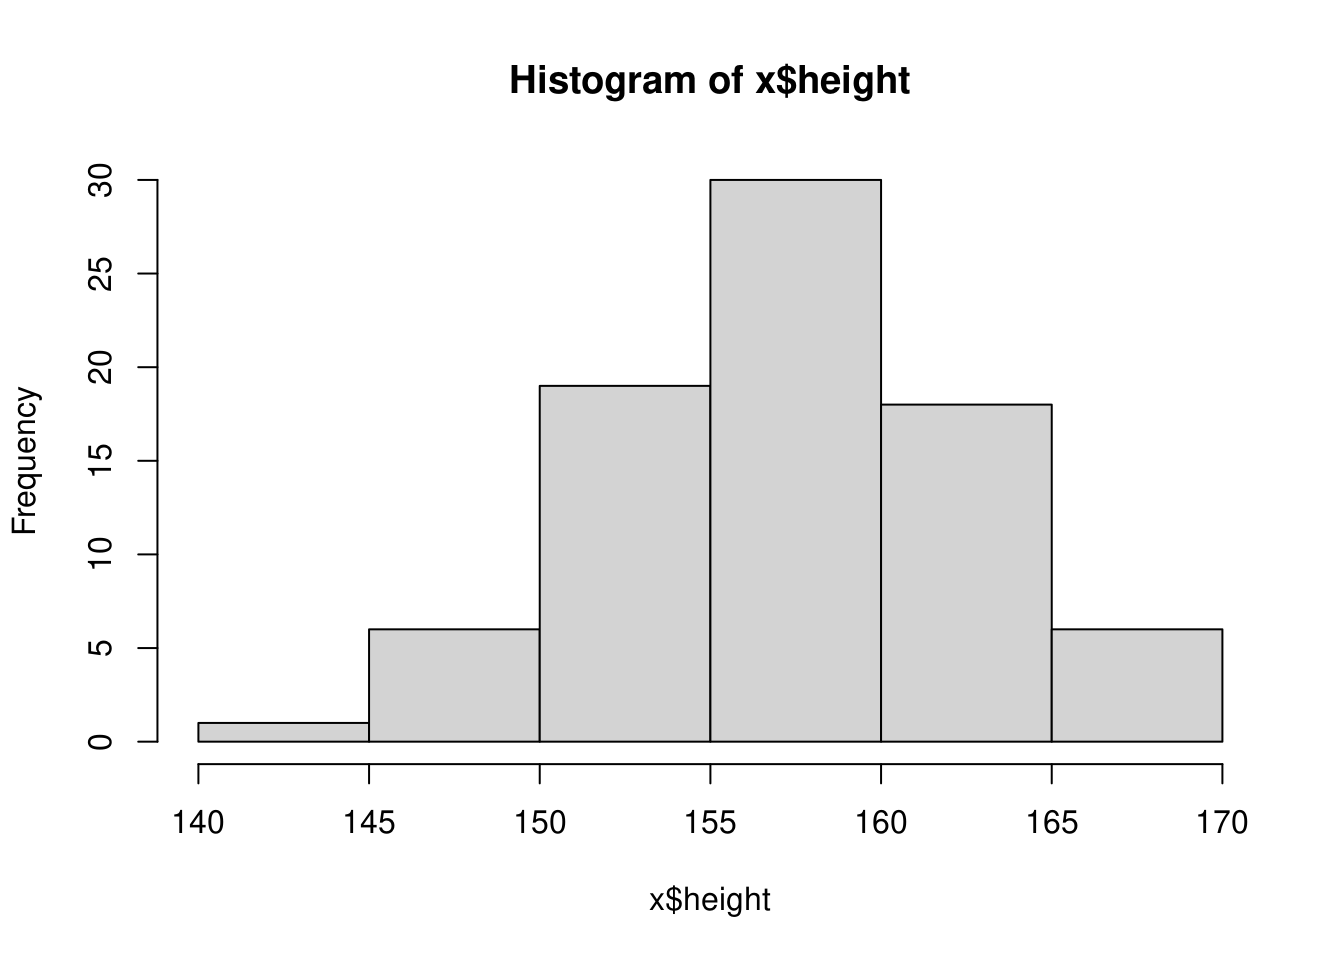
\includegraphics[width=0.9\linewidth,]{R_files/figure-latex/unnamed-chunk-3-1} 

}

\caption{Rのhist()関数}\label{fig:unnamed-chunk-3}
\end{figure}

 \texttt{hist()}関数はヒストグラムを描くために必要となる階級や度数、階級値などの情報を出力することも可能です。

\begin{Shaded}
\begin{Highlighting}[]
\FunctionTok{hist}\NormalTok{(}\AttributeTok{x =}\NormalTok{ x}\SpecialCharTok{$}\NormalTok{height, }\AttributeTok{plot =} \ConstantTok{FALSE}\NormalTok{)}
\end{Highlighting}
\end{Shaded}

\begin{verbatim}
## $breaks
## [1] 140 145 150 155 160 165 170
## 
## $counts
## [1]  1  6 19 30 18  6
## 
## $density
## [1] 0.0025 0.0150 0.0475 0.0750 0.0450 0.0150
## 
## $mids
## [1] 142.5 147.5 152.5 157.5 162.5 167.5
## 
## $xname
## [1] "x$height"
## 
## $equidist
## [1] TRUE
## 
## attr(,"class")
## [1] "histogram"
\end{verbatim}

\begin{longtable}[]{@{}
  >{\raggedright\arraybackslash}p{(\columnwidth - 4\tabcolsep) * \real{0.1618}}
  >{\raggedright\arraybackslash}p{(\columnwidth - 4\tabcolsep) * \real{0.1176}}
  >{\raggedright\arraybackslash}p{(\columnwidth - 4\tabcolsep) * \real{0.7206}}@{}}
\caption{主な出力の意味}\tabularnewline
\toprule
\begin{minipage}[b]{\linewidth}\raggedright
出力名
\end{minipage} & \begin{minipage}[b]{\linewidth}\raggedright
意味
\end{minipage} & \begin{minipage}[b]{\linewidth}\raggedright
備考
\end{minipage} \\
\midrule
\endfirsthead
\toprule
\begin{minipage}[b]{\linewidth}\raggedright
出力名
\end{minipage} & \begin{minipage}[b]{\linewidth}\raggedright
意味
\end{minipage} & \begin{minipage}[b]{\linewidth}\raggedright
備考
\end{minipage} \\
\midrule
\endhead
\texttt{\$breaks} & 階級 & デフォルトはスタージェスの公式\textsuperscript{*}にもとづく区切り(幅) \\
\texttt{\$counts} & 度数 & 各階級に入るデータの個数 \\
\texttt{\$density} & 密度 & 密度推定値 \\
\texttt{\$mids} & 階級値 & 階級の中央値(階級の単純平均) \\
\bottomrule
\end{longtable}

\textsuperscript{*} 後述

 表形式の度数分布表を作成する場合は以下のようにコード処理します。

\begin{Shaded}
\begin{Highlighting}[]
\NormalTok{x }\SpecialCharTok{\%\textgreater{}\%} 
  \CommentTok{\# 階級を求めて、データを階級ごとに分ける}
\NormalTok{  dplyr}\SpecialCharTok{::}\FunctionTok{mutate}\NormalTok{(}\AttributeTok{class =} \FunctionTok{cut}\NormalTok{(height,}
                            \AttributeTok{breaks =} \FunctionTok{pretty}\NormalTok{(height, }\AttributeTok{n =} \FunctionTok{nclass.Sturges}\NormalTok{(height)),}
                            \AttributeTok{include.lowest =} \ConstantTok{FALSE}\NormalTok{, }\AttributeTok{right =} \ConstantTok{TRUE}\NormalTok{)) }\SpecialCharTok{\%\textgreater{}\%} 
  \CommentTok{\# 階級ごとの度数を求める}
\NormalTok{  dplyr}\SpecialCharTok{::}\FunctionTok{count}\NormalTok{(class) }\SpecialCharTok{\%\textgreater{}\%} 
  \CommentTok{\# 累積度数、相対度数、累積相対度数を求める}
\NormalTok{  dplyr}\SpecialCharTok{::}\FunctionTok{mutate}\NormalTok{(}\AttributeTok{cumsum\_n =} \FunctionTok{cumsum}\NormalTok{(n),}
                \AttributeTok{prop =} \FunctionTok{prop.table}\NormalTok{(n), }\AttributeTok{cumsum\_prop =} \FunctionTok{cumsum}\NormalTok{(prop)) }\SpecialCharTok{\%\textgreater{}\%} 
  \CommentTok{\# 階級値を求める}
\NormalTok{  dplyr}\SpecialCharTok{::}\FunctionTok{mutate}\NormalTok{(}\AttributeTok{class\_value =} \FunctionTok{as.character}\NormalTok{(class)) }\SpecialCharTok{\%\textgreater{}\%}
\NormalTok{  tidyr}\SpecialCharTok{::}\FunctionTok{separate}\NormalTok{(class\_value, }\AttributeTok{into =} \FunctionTok{c}\NormalTok{(}\StringTok{"l"}\NormalTok{, }\StringTok{"h"}\NormalTok{), }\AttributeTok{sep =} \StringTok{","}\NormalTok{) }\SpecialCharTok{\%\textgreater{}\%} 
\NormalTok{  dplyr}\SpecialCharTok{::}\FunctionTok{mutate}\NormalTok{(}\AttributeTok{l =} \FunctionTok{as.integer}\NormalTok{(stringr}\SpecialCharTok{::}\FunctionTok{str\_remove}\NormalTok{(l, }\StringTok{"[[:punct:]]"}\NormalTok{)) }\SpecialCharTok{+}\NormalTok{ 1L,}
                \AttributeTok{h =} \FunctionTok{as.integer}\NormalTok{(stringr}\SpecialCharTok{::}\FunctionTok{str\_remove}\NormalTok{(h, }\StringTok{"[[:punct:]]"}\NormalTok{)),}
                \AttributeTok{mids =}\NormalTok{ (l }\SpecialCharTok{+}\NormalTok{ h) }\SpecialCharTok{/}\NormalTok{ 2L) }\SpecialCharTok{\%\textgreater{}\%}
  \CommentTok{\# 変数名を日本語にする}
\NormalTok{  dplyr}\SpecialCharTok{::}\FunctionTok{select}\NormalTok{(}\StringTok{\textasciigrave{}}\AttributeTok{階級}\StringTok{\textasciigrave{}} \OtherTok{=}\NormalTok{ class, }\StringTok{\textasciigrave{}}\AttributeTok{階級値}\StringTok{\textasciigrave{}} \OtherTok{=}\NormalTok{ mids,}
                \StringTok{\textasciigrave{}}\AttributeTok{度数}\StringTok{\textasciigrave{}} \OtherTok{=}\NormalTok{ n, }\StringTok{\textasciigrave{}}\AttributeTok{累積度数}\StringTok{\textasciigrave{}} \OtherTok{=}\NormalTok{ cumsum\_n,}
                \StringTok{\textasciigrave{}}\AttributeTok{相対度数}\StringTok{\textasciigrave{}} \OtherTok{=}\NormalTok{ prop, }\StringTok{\textasciigrave{}}\AttributeTok{累積相対度数}\StringTok{\textasciigrave{}} \OtherTok{=}\NormalTok{ cumsum\_prop)}
\end{Highlighting}
\end{Shaded}

\begin{verbatim}
## # A tibble: 6 x 6
##   階級      階級値  度数 累積度数 相対度数 累積相対度数
##   <fct>      <dbl> <int>    <int>    <dbl>        <dbl>
## 1 (140,145]    143     1        1   0.0125       0.0125
## 2 (145,150]    148     6        7   0.075        0.0875
## 3 (150,155]    153    19       26   0.238        0.325 
## 4 (155,160]    158    30       56   0.375        0.7   
## 5 (160,165]    163    18       74   0.225        0.925 
## 6 (165,170]    168     6       80   0.075        1
\end{verbatim}

 以降の項は度数分布表の作成に必要な関数の使い方を紹介していますので、不要な方は演習問題まで読み飛ばしてください。

 

\hypertarget{ux968eux7d1aux3092ux6c42ux3081ux308b}{%
\subsection{階級を求める}\label{ux968eux7d1aux3092ux6c42ux3081ux308b}}

\begin{quote}
以降に出てくる\texttt{with()}関数は、第一引数で指定するデータフレーム型変数内の変数名を第二引数内で参照演算子(\texttt{\$})を用いることなく参照できるようにする関数です。
\end{quote}

 階級を求めるには\texttt{pretty()}関数を使います。

\begin{Shaded}
\begin{Highlighting}[]
\FunctionTok{with}\NormalTok{(x, }\FunctionTok{pretty}\NormalTok{(}\AttributeTok{x =}\NormalTok{ height, }\AttributeTok{n =} \FunctionTok{nclass.Sturges}\NormalTok{(height)))}
\end{Highlighting}
\end{Shaded}

\begin{verbatim}
## [1] 140 145 150 155 160 165 170
\end{verbatim}

 第一引数\texttt{x}には階級を求めたいベクトル型データを第二引数\texttt{n}には階級を区切りたい数(階級数)を指定します。ここでは、階級数\texttt{n}にはスタージェスの公式から求めた階級数を指定しています。\\
 ただし、必ずしも指定した階級数に分割される訳ではない点に注意してください。\texttt{x}で指定したデータが階級に収まるように適切な丸め処理を行いますので、指定した階級数とは異なる階級が求められることもあります。

 スタージェスの公式は、階級数を\(k\)、データのサイズ(数)を\(n\)とした場合、下式で定義されます。

\[k = \lceil \log_2n + 1 \rceil\]

 スタージェスの公式は\texttt{nclass.Sturgess()}関数として実装されています。

\begin{Shaded}
\begin{Highlighting}[]
\FunctionTok{with}\NormalTok{(x, }\FunctionTok{nclass.Sturges}\NormalTok{(height))}
\end{Highlighting}
\end{Shaded}

\begin{verbatim}
## [1] 8
\end{verbatim}

 スタージェスの公式はヒストグラムを平滑化し過ぎる傾向があると言われています。気になる場合はスコットの選択(\texttt{nclass.scott()})やフリードマン=ダイアコニスの選択(\texttt{nclass.FD()})を試して見てください。

 

\hypertarget{ux30c7ux30fcux30bfux3092ux5404ux968eux7d1aux306bux5206ux985eux3059ux308b}{%
\subsection{データを各階級に分類する}\label{ux30c7ux30fcux30bfux3092ux5404ux968eux7d1aux306bux5206ux985eux3059ux308b}}

 データを階級分けするには\texttt{cut()}関数を使います。

\begin{Shaded}
\begin{Highlighting}[]
\FunctionTok{with}\NormalTok{(x, }\FunctionTok{cut}\NormalTok{(}\AttributeTok{x =}\NormalTok{ height, }\AttributeTok{breaks =} \FunctionTok{pretty}\NormalTok{(height, }\AttributeTok{n =} \FunctionTok{nclass.Sturges}\NormalTok{(height))))}
\end{Highlighting}
\end{Shaded}

\begin{verbatim}
##  [1] (150,155] (150,155] (155,160] (155,160] (160,165] (155,160] (155,160]
##  [8] (155,160] (150,155] (155,160] (150,155] (160,165] (155,160] (160,165]
## [15] (155,160] (160,165] (160,165] (165,170] (145,150] (160,165] (150,155]
## [22] (160,165] (155,160] (160,165] (165,170] (150,155] (155,160] (150,155]
## [29] (155,160] (155,160] (155,160] (145,150] (160,165] (150,155] (155,160]
## [36] (160,165] (150,155] (160,165] (150,155] (150,155] (150,155] (150,155]
## [43] (155,160] (145,150] (145,150] (160,165] (165,170] (150,155] (150,155]
## [50] (165,170] (160,165] (160,165] (145,150] (140,145] (155,160] (160,165]
## [57] (155,160] (155,160] (155,160] (160,165] (165,170] (155,160] (155,160]
## [64] (150,155] (155,160] (155,160] (150,155] (155,160] (150,155] (155,160]
## [71] (145,150] (165,170] (150,155] (155,160] (155,160] (155,160] (160,165]
## [78] (155,160] (155,160] (160,165]
## Levels: (140,145] (145,150] (150,155] (155,160] (160,165] (165,170]
\end{verbatim}

 第一引数\texttt{x}には階級分けの対象となるベクトル型変数を第二引数\texttt{breaks}には前項で求めた階級を指定します。\texttt{breaks}引数には任意の階級、例えば\texttt{breaks\ =\ c(140,\ 155,\ 170)}のように指定することも可能です。

 

\hypertarget{ux968eux7d1aux306eux5883ux754cux5024ux306fux3069ux3061ux3089ux306bux542bux307eux308cux308bux306eux304b}{%
\subsubsection*{階級の境界値はどちらに含まれるのか?}\label{ux968eux7d1aux306eux5883ux754cux5024ux306fux3069ux3061ux3089ux306bux542bux307eux308cux308bux306eux304b}}
\addcontentsline{toc}{subsubsection}{階級の境界値はどちらに含まれるのか?}

 \texttt{cut()}関数の出力は、\texttt{(140,145{]}\ (145,150{]}}のように階級間で同じ数値、この場合は\texttt{145}が含まれます。では、\texttt{145}はどちらの階級に含まれるのでしょうか?答えは、添えられている括弧にあります。

\begin{quote}
\texttt{(140,145{]}}
\end{quote}

は「140を超えて145以下」となりますので、次の

\begin{quote}
\texttt{(145,150{]}}
\end{quote}

は同様に「145を超えて150以下」となります。階級間の境界値である\texttt{145}は\texttt{(140,\ 145{]}}側に入ります。

\begin{quote}
\texttt{(}は「超えて」(境界値を含まない)、\texttt{{]}}は「以下」(境界値を含む)
\end{quote}

で、逆向きの場合は

\begin{quote}
\texttt{)}は「未満」(境界値を含まない)、\texttt{{[}}は「以上」(境界値を含む)
\end{quote}

となります。\texttt{hist()}関数の階級も同様です。

 境界値をどちらに含めるかは\texttt{include.lowest}引数と\texttt{right}引数で指定できます。

\begin{longtable}[]{@{}
  >{\raggedright\arraybackslash}p{(\columnwidth - 4\tabcolsep) * \real{0.4167}}
  >{\raggedright\arraybackslash}p{(\columnwidth - 4\tabcolsep) * \real{0.3194}}
  >{\raggedright\arraybackslash}p{(\columnwidth - 4\tabcolsep) * \real{0.2639}}@{}}
\toprule
\begin{minipage}[b]{\linewidth}\raggedright
option
\end{minipage} & \begin{minipage}[b]{\linewidth}\raggedright
\texttt{right\ =\ TRUE}  
\end{minipage} & \begin{minipage}[b]{\linewidth}\raggedright
\texttt{right\ =\ FALSE}
\end{minipage} \\
\midrule
\endhead
\textbf{\texttt{include.lowest\ =\ TRUE}} & \texttt{{[}l,u{]}\ ...\ (l,u{]}} & \texttt{{[}l,u)\ ...\ {[}l,u{]}} \\
\textbf{\texttt{include.lowest\ =\ FALSE}} & \texttt{(l,u{]}\ ...\ (l,u{]}}\textsuperscript{*} & \texttt{{[}l,u)\ ...\ {[}l,u)} \\
\bottomrule
\end{longtable}

 \textsuperscript{*}デフォルト

 例えばデータの最大値と最小値を境界値として含む階級を指定した場合、\texttt{include.lowest\ =\ FALSE,\ right\ =\ FALSE}と指定すると最大値が階級に含まれなくなります。

\begin{Shaded}
\begin{Highlighting}[]
\FunctionTok{with}\NormalTok{(x, }\FunctionTok{cut}\NormalTok{(height, }\AttributeTok{breaks =} \FunctionTok{c}\NormalTok{(}\DecValTok{143}\NormalTok{, }\DecValTok{155}\NormalTok{, }\DecValTok{169}\NormalTok{),}
            \AttributeTok{include.lowest =} \ConstantTok{FALSE}\NormalTok{, }\AttributeTok{right =} \ConstantTok{FALSE}\NormalTok{))}
\end{Highlighting}
\end{Shaded}

\begin{verbatim}
##  [1] [143,155) [143,155) [155,169) [155,169) [155,169) [155,169) [155,169)
##  [8] [155,169) [143,155) [155,169) [143,155) [155,169) [155,169) [155,169)
## [15] [155,169) [155,169) [155,169) <NA>      [143,155) [155,169) [143,155)
## [22] [155,169) [155,169) [155,169) [155,169) [143,155) [155,169) [155,169)
## [29] [155,169) [155,169) [155,169) [143,155) [155,169) [155,169) [155,169)
## [36] [155,169) [143,155) [155,169) [143,155) [143,155) [143,155) [155,169)
## [43] [155,169) [143,155) [143,155) [155,169) <NA>      [143,155) [155,169)
## [50] [155,169) [155,169) [155,169) [143,155) [143,155) [155,169) [155,169)
## [57] [155,169) [155,169) [155,169) [155,169) [155,169) [155,169) [155,169)
## [64] [143,155) [155,169) [155,169) [143,155) [155,169) [143,155) [155,169)
## [71] [143,155) [155,169) [143,155) [155,169) [155,169) [155,169) [155,169)
## [78] [155,169) [155,169) [155,169)
## Levels: [143,155) [155,169)
\end{verbatim}

 逆に\texttt{include.lowest\ =\ FALSE,\ right\ =\ TRUE}と指定すると最小値が階級に含まれなくなります。

\begin{Shaded}
\begin{Highlighting}[]
\FunctionTok{with}\NormalTok{(x, }\FunctionTok{cut}\NormalTok{(height, }\AttributeTok{breaks =} \FunctionTok{c}\NormalTok{(}\DecValTok{143}\NormalTok{, }\DecValTok{155}\NormalTok{, }\DecValTok{169}\NormalTok{),}
            \AttributeTok{include.lowest =} \ConstantTok{FALSE}\NormalTok{, }\AttributeTok{right =} \ConstantTok{TRUE}\NormalTok{))}
\end{Highlighting}
\end{Shaded}

\begin{verbatim}
##  [1] (143,155] (143,155] (155,169] (155,169] (155,169] (155,169] (155,169]
##  [8] (155,169] (143,155] (155,169] (143,155] (155,169] (155,169] (155,169]
## [15] (155,169] (155,169] (155,169] (155,169] (143,155] (155,169] (143,155]
## [22] (155,169] (155,169] (155,169] (155,169] (143,155] (155,169] (143,155]
## [29] (155,169] (155,169] (155,169] (143,155] (155,169] (143,155] (155,169]
## [36] (155,169] (143,155] (155,169] (143,155] (143,155] (143,155] (143,155]
## [43] (155,169] (143,155] (143,155] (155,169] (155,169] (143,155] (143,155]
## [50] (155,169] (155,169] (155,169] (143,155] <NA>      (155,169] (155,169]
## [57] (155,169] (155,169] (155,169] (155,169] (155,169] (155,169] (155,169]
## [64] (143,155] (155,169] (155,169] (143,155] (155,169] (143,155] (155,169]
## [71] (143,155] (155,169] (143,155] (155,169] (155,169] (155,169] (155,169]
## [78] (155,169] (155,169] (155,169]
## Levels: (143,155] (155,169]
\end{verbatim}

 

\hypertarget{ux5ea6ux6570ux3092ux6c42ux3081ux308b}{%
\subsection{度数を求める}\label{ux5ea6ux6570ux3092ux6c42ux3081ux308b}}

 度数を求めるには各階級の数を数えます。数を数えるには\texttt{table()}関数や\texttt{dplyr::count()}関数を使います。\texttt{table()}関数はベクトル型を対象に、\texttt{dplyr::count()}関数はデータフレーム型を対象として個数をカウントします。用途によって使い分けてください。

\begin{Shaded}
\begin{Highlighting}[]
\FunctionTok{with}\NormalTok{(x, }\FunctionTok{table}\NormalTok{(}\FunctionTok{cut}\NormalTok{(height, }\AttributeTok{breaks =} \FunctionTok{pretty}\NormalTok{(height, }\AttributeTok{n =} \FunctionTok{nclass.Sturges}\NormalTok{(height)))))}
\end{Highlighting}
\end{Shaded}

\begin{verbatim}
## 
## (140,145] (145,150] (150,155] (155,160] (160,165] (165,170] 
##         1         6        19        30        18         6
\end{verbatim}

 

\begin{Shaded}
\begin{Highlighting}[]
\NormalTok{x }\SpecialCharTok{\%\textgreater{}\%} 
  \CommentTok{\# 階級を求めて、データを階級ごとに分ける}
\NormalTok{  dplyr}\SpecialCharTok{::}\FunctionTok{mutate}\NormalTok{(}\AttributeTok{class =} \FunctionTok{cut}\NormalTok{(height,}
                            \AttributeTok{breaks =} \FunctionTok{pretty}\NormalTok{(height, }\AttributeTok{n =} \FunctionTok{nclass.Sturges}\NormalTok{(height)))) }\SpecialCharTok{\%\textgreater{}\%} 
  \CommentTok{\# 階級ごとの度数を求める}
\NormalTok{  dplyr}\SpecialCharTok{::}\FunctionTok{count}\NormalTok{(class)}
\end{Highlighting}
\end{Shaded}

\begin{verbatim}
## # A tibble: 6 x 2
##   class         n
##   <fct>     <int>
## 1 (140,145]     1
## 2 (145,150]     6
## 3 (150,155]    19
## 4 (155,160]    30
## 5 (160,165]    18
## 6 (165,170]     6
\end{verbatim}

 

\hypertarget{ux7d2fux7a4dux5ea6ux6570ux76f8ux5bfeux5ea6ux6570ux7d2fux7a4dux76f8ux5bfeux5ea6ux6570ux3092ux6c42ux3081ux308b}{%
\subsection{累積度数、相対度数、累積相対度数を求める}\label{ux7d2fux7a4dux5ea6ux6570ux76f8ux5bfeux5ea6ux6570ux7d2fux7a4dux76f8ux5bfeux5ea6ux6570ux3092ux6c42ux3081ux308b}}

 累積度数(度数の累積和)を求めるには\texttt{cumsum()}関数を使います。

\begin{Shaded}
\begin{Highlighting}[]
\FunctionTok{with}\NormalTok{(x, }\FunctionTok{cumsum}\NormalTok{(}\FunctionTok{table}\NormalTok{(}\FunctionTok{cut}\NormalTok{(height, }\AttributeTok{breaks =} \FunctionTok{pretty}\NormalTok{(height, }\AttributeTok{n =} \FunctionTok{nclass.Sturges}\NormalTok{(height))))))}
\end{Highlighting}
\end{Shaded}

\begin{verbatim}
## (140,145] (145,150] (150,155] (155,160] (160,165] (165,170] 
##         1         7        26        56        74        80
\end{verbatim}

 

 相対度数を求めるには\texttt{prop.table()}関数を使います。

\begin{Shaded}
\begin{Highlighting}[]
\FunctionTok{with}\NormalTok{(x, }\FunctionTok{prop.table}\NormalTok{(}\FunctionTok{table}\NormalTok{(}\FunctionTok{cut}\NormalTok{(height, }\AttributeTok{breaks =} \FunctionTok{pretty}\NormalTok{(height, }\AttributeTok{n =} \FunctionTok{nclass.Sturges}\NormalTok{(height))))))}
\end{Highlighting}
\end{Shaded}

\begin{verbatim}
## 
## (140,145] (145,150] (150,155] (155,160] (160,165] (165,170] 
##    0.0125    0.0750    0.2375    0.3750    0.2250    0.0750
\end{verbatim}

 

 累積相対度数は相対度数の累積和ですので、\texttt{prop.table()}関数の結果を\texttt{cumsum()}関数に渡すことで求めることができます。

\begin{Shaded}
\begin{Highlighting}[]
\FunctionTok{with}\NormalTok{(x, }\FunctionTok{cumsum}\NormalTok{(}\FunctionTok{prop.table}\NormalTok{(}\FunctionTok{table}\NormalTok{(}\FunctionTok{cut}\NormalTok{(height, }\AttributeTok{breaks =} \FunctionTok{pretty}\NormalTok{(height, }\AttributeTok{n =} \FunctionTok{nclass.Sturges}\NormalTok{(height)))))))}
\end{Highlighting}
\end{Shaded}

\begin{verbatim}
## (140,145] (145,150] (150,155] (155,160] (160,165] (165,170] 
##    0.0125    0.0875    0.3250    0.7000    0.9250    1.0000
\end{verbatim}

 

\hypertarget{ux968eux7d1aux5024ux3092ux6c42ux3081ux308b}{%
\subsection{階級値を求める}\label{ux968eux7d1aux5024ux3092ux6c42ux3081ux308b}}

 階級値は階級の文字列から下端と上端の境界値を抜き出し、下式で単純平均として求めています。

\[\frac{(\mbox{下端} + 1) + \mbox{上端}}{2}\]

 手順としては以下のようにしています。

\begin{enumerate}
\def\labelenumi{\arabic{enumi}.}
\tightlist
\item
  \texttt{as.character()}関数で 階級(\texttt{class})を文字型に変換し、新しい変数(\texttt{class\_value})を作成する\\
\item
  \texttt{tidyr::separate()}関数で文字型の変数(\texttt{class\_value})を\texttt{,}の前後で二つの変数(\texttt{l}, \texttt{h})に分割する\\
\item
  \texttt{stringr::str\_remove}関数で二つの変数(\texttt{l}, \texttt{h})から\texttt{(}や\texttt{{]}}を取り除き\texttt{as.numeric()}関数で文字列から数値に変換する\\
\item
  数値に変換された二つの変数から(\texttt{l}, \texttt{h})平均値を求める
\end{enumerate}

\begin{Shaded}
\begin{Highlighting}[]
\NormalTok{x }\SpecialCharTok{\%\textgreater{}\%} 
  \CommentTok{\# 階級を求めて、データを階級ごとに分ける}
\NormalTok{  dplyr}\SpecialCharTok{::}\FunctionTok{mutate}\NormalTok{(}\AttributeTok{class =} \FunctionTok{cut}\NormalTok{(height,}
                            \AttributeTok{breaks =} \FunctionTok{pretty}\NormalTok{(height, }\AttributeTok{n =} \FunctionTok{nclass.Sturges}\NormalTok{(height)),}
                            \AttributeTok{include.lowest =} \ConstantTok{FALSE}\NormalTok{, }\AttributeTok{right =} \ConstantTok{TRUE}\NormalTok{)) }\SpecialCharTok{\%\textgreater{}\%} 
  \CommentTok{\# 階級ごとの度数を求める}
\NormalTok{  dplyr}\SpecialCharTok{::}\FunctionTok{count}\NormalTok{(class) }\SpecialCharTok{\%\textgreater{}\%} 
  \CommentTok{\# 階級値を求める}
\NormalTok{  dplyr}\SpecialCharTok{::}\FunctionTok{mutate}\NormalTok{(}\AttributeTok{class\_value =} \FunctionTok{as.character}\NormalTok{(class)) }\SpecialCharTok{\%\textgreater{}\%} 
\NormalTok{  tidyr}\SpecialCharTok{::}\FunctionTok{separate}\NormalTok{(class\_value, }\AttributeTok{into =} \FunctionTok{c}\NormalTok{(}\StringTok{"l"}\NormalTok{, }\StringTok{"h"}\NormalTok{), }\AttributeTok{sep =} \StringTok{","}\NormalTok{) }\SpecialCharTok{\%\textgreater{}\%} 
\NormalTok{  dplyr}\SpecialCharTok{::}\FunctionTok{mutate}\NormalTok{(}\AttributeTok{l =} \FunctionTok{as.numeric}\NormalTok{(stringr}\SpecialCharTok{::}\FunctionTok{str\_remove}\NormalTok{(l, }\StringTok{"[[:punct:]]"}\NormalTok{)),}
                \AttributeTok{h =} \FunctionTok{as.numeric}\NormalTok{(stringr}\SpecialCharTok{::}\FunctionTok{str\_remove}\NormalTok{(h, }\StringTok{"[[:punct:]]"}\NormalTok{))) }\SpecialCharTok{\%\textgreater{}\%} 
\NormalTok{  dplyr}\SpecialCharTok{::}\FunctionTok{mutate}\NormalTok{(}\AttributeTok{mids =}\NormalTok{ ((l }\SpecialCharTok{+} \DecValTok{1}\NormalTok{) }\SpecialCharTok{+}\NormalTok{ h) }\SpecialCharTok{/} \DecValTok{2}\NormalTok{)}
\end{Highlighting}
\end{Shaded}

\begin{verbatim}
## # A tibble: 6 x 5
##   class         n     l     h  mids
##   <fct>     <int> <dbl> <dbl> <dbl>
## 1 (140,145]     1   140   145   143
## 2 (145,150]     6   145   150   148
## 3 (150,155]    19   150   155   153
## 4 (155,160]    30   155   160   158
## 5 (160,165]    18   160   165   163
## 6 (165,170]     6   165   170   168
\end{verbatim}

 

\hypertarget{ux7df4ux7fd2ux554fux984c}{%
\section{練習問題}\label{ux7df4ux7fd2ux554fux984c}}

 テキストP23にあるデータで度数分布表とヒストグラムを作成する。

\begin{verbatim}
## # A tibble: 10 x 8
##       X1    X2    X3    X4    X5    X6    X7    X8
##    <dbl> <dbl> <dbl> <dbl> <dbl> <dbl> <dbl> <dbl>
##  1    48    54    47    50    53    43    45    43
##  2    44    47    58    46    46    63    49    50
##  3    48    43    46    45    50    53    51    58
##  4    52    53    47    49    45    42    51    49
##  5    58    54    45    53    50    69    44    50
##  6    58    64    40    57    51    69    58    47
##  7    62    47    40    60    48    47    53    47
##  8    52    61    55    55    48    48    46    52
##  9    45    38    62    47    55    50    46    47
## 10    55    48    50    50    54    55    48    50
\end{verbatim}

 

\hypertarget{ux89e3ux7b54ux4f8b}{%
\subsection*{解答例}\label{ux89e3ux7b54ux4f8b}}
\addcontentsline{toc}{subsection}{解答例}

 まず、処理しやすいように下記のように対象データを変形し\texttt{df}というデータフレーム型の変数に格納しておきます。

\begin{Shaded}
\begin{Highlighting}[]
\NormalTok{df}
\end{Highlighting}
\end{Shaded}

\begin{verbatim}
## # A tibble: 80 x 1
##    weight
##     <int>
##  1     48
##  2     44
##  3     48
##  4     52
##  5     58
##  6     58
##  7     62
##  8     52
##  9     45
## 10     55
## # ... with 70 more rows
\end{verbatim}

 度数分布表を身長の場合と同じ要領で作成します。

\begin{Shaded}
\begin{Highlighting}[]
\NormalTok{df }\SpecialCharTok{\%\textgreater{}\%} 
  \CommentTok{\# 階級を求めて、データを階級ごとに分ける}
\NormalTok{  dplyr}\SpecialCharTok{::}\FunctionTok{mutate}\NormalTok{(}\AttributeTok{class =} \FunctionTok{cut}\NormalTok{(weight,}
                            \AttributeTok{breaks =} \FunctionTok{pretty}\NormalTok{(weight, }\AttributeTok{n =} \FunctionTok{nclass.Sturges}\NormalTok{(weight)),}
                            \AttributeTok{include.lowest =} \ConstantTok{FALSE}\NormalTok{, }\AttributeTok{right =} \ConstantTok{TRUE}\NormalTok{)) }\SpecialCharTok{\%\textgreater{}\%} 
  \CommentTok{\# 階級ごとの度数を求める}
\NormalTok{  dplyr}\SpecialCharTok{::}\FunctionTok{count}\NormalTok{(class) }\SpecialCharTok{\%\textgreater{}\%} 
  \CommentTok{\# 累積度数、相対度数、累積相対度数を求める}
\NormalTok{  dplyr}\SpecialCharTok{::}\FunctionTok{mutate}\NormalTok{(}\AttributeTok{cumsum\_n =} \FunctionTok{cumsum}\NormalTok{(n),}
                \AttributeTok{prop =} \FunctionTok{prop.table}\NormalTok{(n), }\AttributeTok{cumsum\_prop =} \FunctionTok{cumsum}\NormalTok{(prop)) }\SpecialCharTok{\%\textgreater{}\%} 
  \CommentTok{\# 階級値を求める}
\NormalTok{  dplyr}\SpecialCharTok{::}\FunctionTok{mutate}\NormalTok{(}\AttributeTok{class\_value =} \FunctionTok{as.character}\NormalTok{(class)) }\SpecialCharTok{\%\textgreater{}\%}
\NormalTok{  tidyr}\SpecialCharTok{::}\FunctionTok{separate}\NormalTok{(class\_value, }\AttributeTok{into =} \FunctionTok{c}\NormalTok{(}\StringTok{"l"}\NormalTok{, }\StringTok{"h"}\NormalTok{), }\AttributeTok{sep =} \StringTok{","}\NormalTok{) }\SpecialCharTok{\%\textgreater{}\%} 
\NormalTok{  dplyr}\SpecialCharTok{::}\FunctionTok{mutate}\NormalTok{(}\AttributeTok{l =} \FunctionTok{as.integer}\NormalTok{(stringr}\SpecialCharTok{::}\FunctionTok{str\_remove}\NormalTok{(l, }\StringTok{"[[:punct:]]"}\NormalTok{)) }\SpecialCharTok{+}\NormalTok{ 1L,}
                \AttributeTok{h =} \FunctionTok{as.integer}\NormalTok{(stringr}\SpecialCharTok{::}\FunctionTok{str\_remove}\NormalTok{(h, }\StringTok{"[[:punct:]]"}\NormalTok{)),}
                \AttributeTok{mids =}\NormalTok{ (l }\SpecialCharTok{+}\NormalTok{ h) }\SpecialCharTok{/}\NormalTok{ 2L) }\SpecialCharTok{\%\textgreater{}\%}
  \CommentTok{\# 変数名を日本語にする}
\NormalTok{  dplyr}\SpecialCharTok{::}\FunctionTok{select}\NormalTok{(}\StringTok{\textasciigrave{}}\AttributeTok{階級}\StringTok{\textasciigrave{}} \OtherTok{=}\NormalTok{ class, }\StringTok{\textasciigrave{}}\AttributeTok{階級値}\StringTok{\textasciigrave{}} \OtherTok{=}\NormalTok{ mids,}
                \StringTok{\textasciigrave{}}\AttributeTok{度数}\StringTok{\textasciigrave{}} \OtherTok{=}\NormalTok{ n, }\StringTok{\textasciigrave{}}\AttributeTok{累積度数}\StringTok{\textasciigrave{}} \OtherTok{=}\NormalTok{ cumsum\_n,}
                \StringTok{\textasciigrave{}}\AttributeTok{相対度数}\StringTok{\textasciigrave{}} \OtherTok{=}\NormalTok{ prop, }\StringTok{\textasciigrave{}}\AttributeTok{累積相対度数}\StringTok{\textasciigrave{}} \OtherTok{=}\NormalTok{ cumsum\_prop)}
\end{Highlighting}
\end{Shaded}

\begin{verbatim}
## # A tibble: 7 x 6
##   階級    階級値  度数 累積度数 相対度数 累積相対度数
##   <fct>    <dbl> <int>    <int>    <dbl>        <dbl>
## 1 (35,40]     38     3        3   0.0375       0.0375
## 2 (40,45]     43    11       14   0.138        0.175 
## 3 (45,50]     48    33       47   0.412        0.588 
## 4 (50,55]     53    19       66   0.238        0.825 
## 5 (55,60]     58     7       73   0.0875       0.912 
## 6 (60,65]     63     5       78   0.0625       0.975 
## 7 (65,70]     68     2       80   0.025        1
\end{verbatim}

 

 ヒストグラムを描きます。

\begin{Shaded}
\begin{Highlighting}[]
\FunctionTok{with}\NormalTok{(df, }\FunctionTok{hist}\NormalTok{(weight))}
\end{Highlighting}
\end{Shaded}

\begin{figure}[H]

{\centering 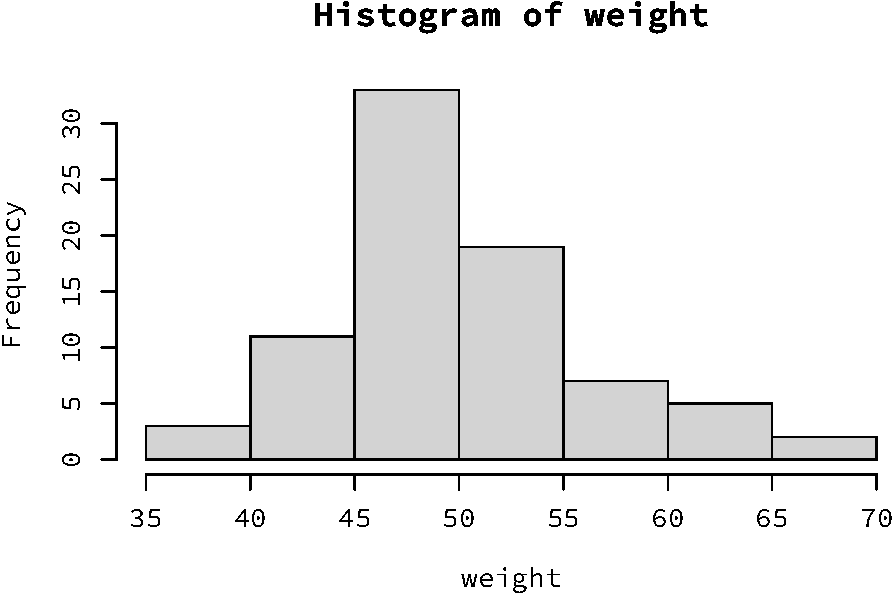
\includegraphics[width=0.9\linewidth,]{R_files/figure-latex/unnamed-chunk-21-1} 

}

\caption{解答例}\label{fig:unnamed-chunk-21}
\end{figure}

 

以上

 

\hypertarget{ux30d2ux30b9ux30c8ux30b0ux30e9ux30e0ux3092ux63cfux304fux30ddux30a4ux30f3ux30c8}{%
\section*{ヒストグラムを描くポイント}\label{ux30d2ux30b9ux30c8ux30b0ux30e9ux30e0ux3092ux63cfux304fux30ddux30a4ux30f3ux30c8}}
\addcontentsline{toc}{section}{ヒストグラムを描くポイント}

 ヒストグラムを描く(度数分布表を作成する)際のポイントは下記の点です。

\begin{enumerate}
\def\labelenumi{\arabic{enumi}.}
\tightlist
\item
  階級の決め方
\item
  階級の境界の扱い
\end{enumerate}

 

\hypertarget{ux968eux7d1aux306eux6c7aux3081ux65b9}{%
\subsection*{階級の決め方}\label{ux968eux7d1aux306eux6c7aux3081ux65b9}}
\addcontentsline{toc}{subsection}{階級の決め方}

 階級を決める方法は特に定められていません。データが取る幅を見て切のよい値にすることが多いようです。ただし、階級のとり方によりヒストグラムの形状が変わる点には注意が必要です。例えば、身長データに対する階級をテキストと同様に\(5cm\)幅とした場合は下図のような形状になります。

\begin{Shaded}
\begin{Highlighting}[]
\FunctionTok{with}\NormalTok{(x, }\FunctionTok{hist}\NormalTok{(height, }\AttributeTok{breaks =} \FunctionTok{seq}\NormalTok{(}\AttributeTok{from =} \DecValTok{140}\NormalTok{, }\AttributeTok{to =} \DecValTok{170}\NormalTok{, }\AttributeTok{by =} \DecValTok{5}\NormalTok{)))}
\end{Highlighting}
\end{Shaded}

\begin{figure}[H]

{\centering 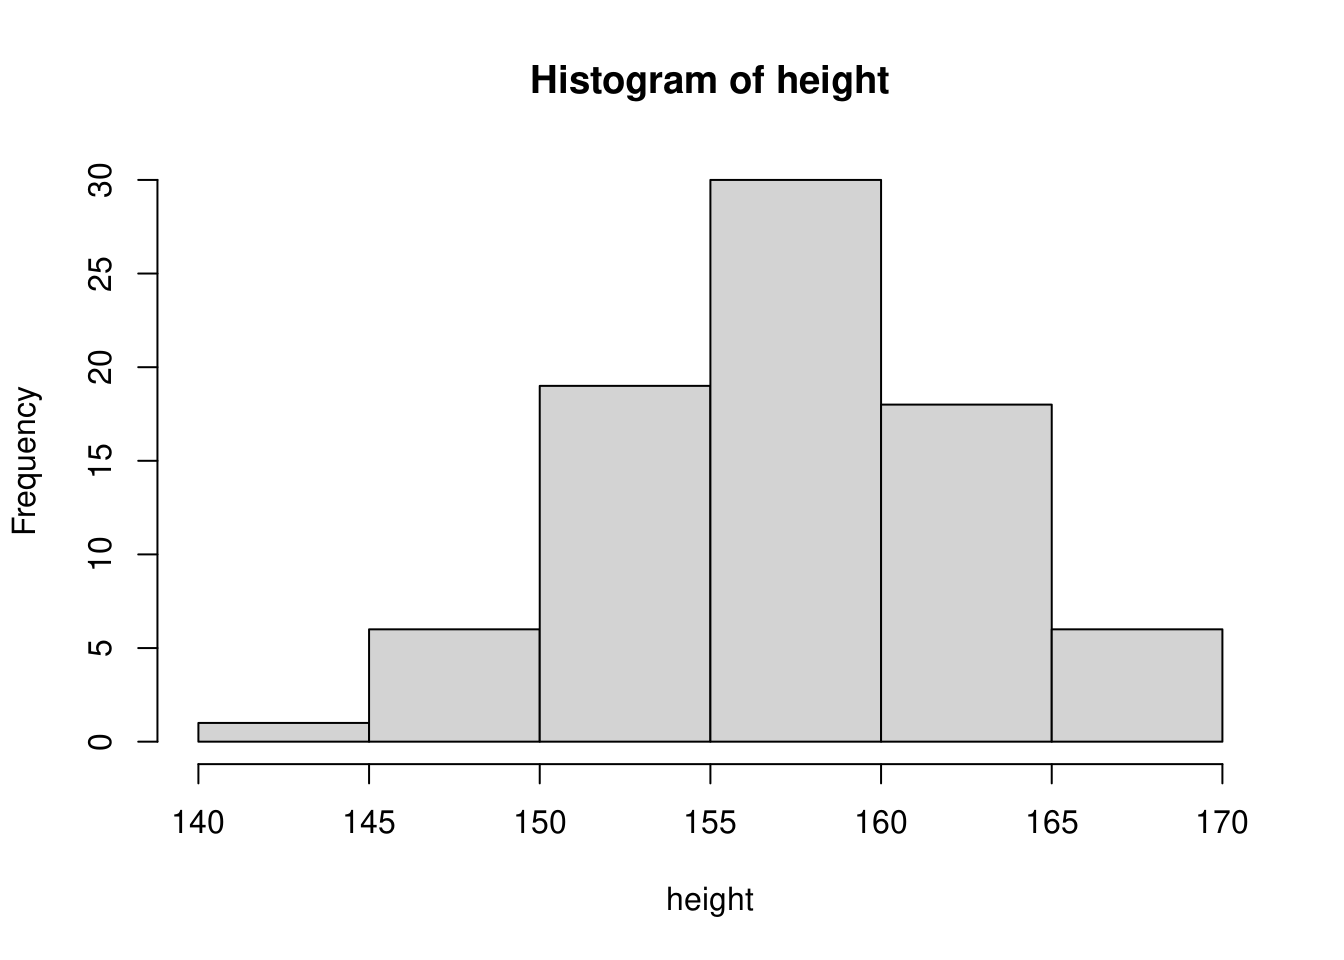
\includegraphics[width=0.9\linewidth,]{R_files/figure-latex/unnamed-chunk-22-1} 

}

\caption{階級幅5cmの場合}\label{fig:unnamed-chunk-22}
\end{figure}

 階級を倍の\(10cm\)幅とすると下図のようになります。

\begin{Shaded}
\begin{Highlighting}[]
\FunctionTok{with}\NormalTok{(x, }\FunctionTok{hist}\NormalTok{(height, }\AttributeTok{breaks =} \FunctionTok{seq}\NormalTok{(}\AttributeTok{from =} \DecValTok{140}\NormalTok{, }\AttributeTok{to =} \DecValTok{170}\NormalTok{, }\AttributeTok{by =} \DecValTok{10}\NormalTok{)))}
\end{Highlighting}
\end{Shaded}

\begin{figure}[H]

{\centering 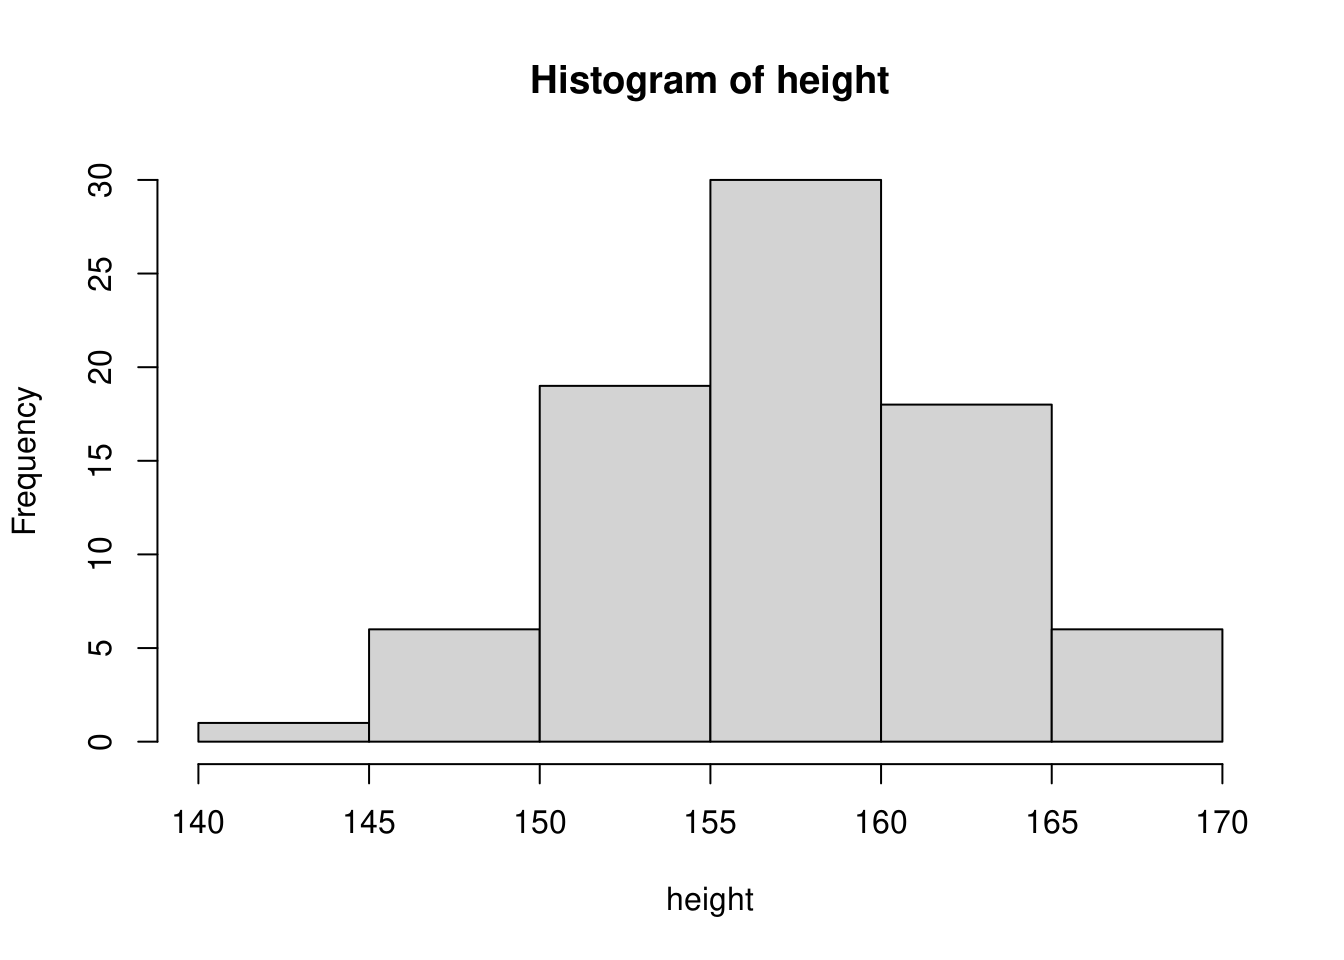
\includegraphics[width=0.9\linewidth,]{R_files/figure-latex/unnamed-chunk-23-1} 

}

\caption{階級幅10cmの場合}\label{fig:unnamed-chunk-23}
\end{figure}

 逆に階級を半分の\(2.5cm\)幅とすると下図のようになります。

\begin{Shaded}
\begin{Highlighting}[]
\FunctionTok{with}\NormalTok{(x, }\FunctionTok{hist}\NormalTok{(height, }\AttributeTok{breaks =} \FunctionTok{seq}\NormalTok{(}\AttributeTok{from =} \DecValTok{140}\NormalTok{, }\AttributeTok{to =} \DecValTok{170}\NormalTok{, }\AttributeTok{by =} \FloatTok{2.5}\NormalTok{)))}
\end{Highlighting}
\end{Shaded}

\begin{figure}[H]

{\centering 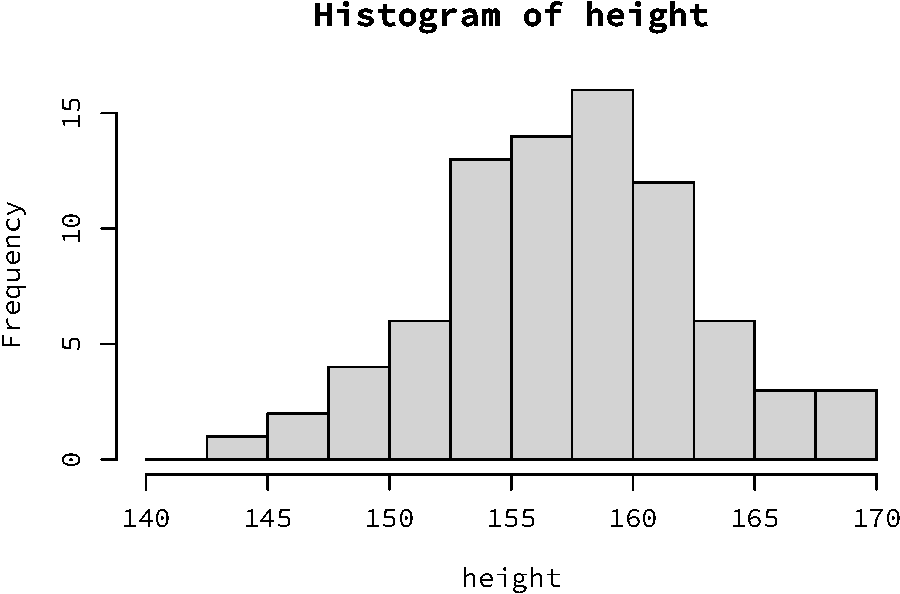
\includegraphics[width=0.9\linewidth,]{R_files/figure-latex/unnamed-chunk-24-1} 

}

\caption{階級幅2.5cmの場合}\label{fig:unnamed-chunk-24}
\end{figure}

 更に細かくして\(1cm\)幅にすると下図のように歯抜けがある形状になります。

\begin{Shaded}
\begin{Highlighting}[]
\FunctionTok{with}\NormalTok{(x, }\FunctionTok{hist}\NormalTok{(height, }\AttributeTok{breaks =} \FunctionTok{seq}\NormalTok{(}\AttributeTok{from =} \DecValTok{140}\NormalTok{, }\AttributeTok{to =} \DecValTok{170}\NormalTok{, }\AttributeTok{by =} \FloatTok{1.0}\NormalTok{)))}
\end{Highlighting}
\end{Shaded}

\begin{figure}[H]

{\centering 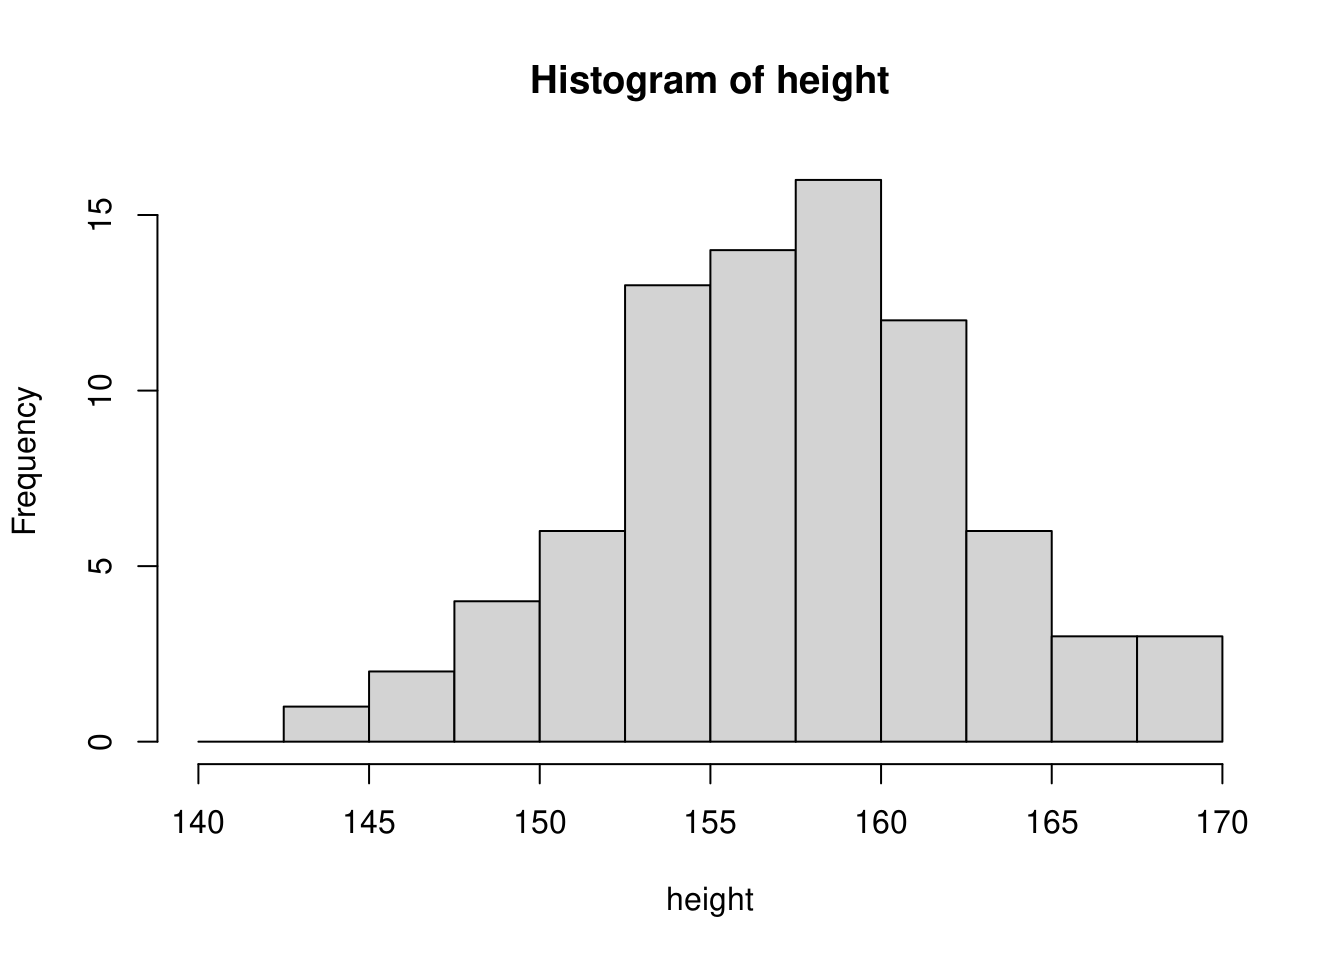
\includegraphics[width=0.9\linewidth,]{R_files/figure-latex/unnamed-chunk-25-1} 

}

\caption{階級幅1cmの場合}\label{fig:unnamed-chunk-25}
\end{figure}

 このように階級の決め方次第でヒストグラムの形状が変わってくることが分かります。ヒストグラムはデータの分布をみるために使うグラフですので、過大な階級幅や過小な階級幅で描くことは好ましくありませんので、適切な値を選ぶようにしてください。

 

\hypertarget{ux8a08ux7b97ux3067ux968eux7d1aux3092ux6c7aux3081ux308b}{%
\subsubsection*{計算で階級を決める}\label{ux8a08ux7b97ux3067ux968eux7d1aux3092ux6c7aux3081ux308b}}
\addcontentsline{toc}{subsubsection}{計算で階級を決める}

 適切な階級をどのように決めれば良いか迷う場合には、下表のような計算方法が提案されていますのでこれらを試してみてください。

\begin{longtable}[]{@{}
  >{\raggedright\arraybackslash}p{(\columnwidth - 4\tabcolsep) * \real{0.4301}}
  >{\raggedright\arraybackslash}p{(\columnwidth - 4\tabcolsep) * \real{0.4301}}
  >{\raggedright\arraybackslash}p{(\columnwidth - 4\tabcolsep) * \real{0.1398}}@{}}
\toprule
\begin{minipage}[b]{\linewidth}\raggedright
階級の求め方
\end{minipage} & \begin{minipage}[b]{\linewidth}\raggedright
階級数(\(k\))・階級幅(\(h\))
\end{minipage} & \begin{minipage}[b]{\linewidth}\raggedright
備考
\end{minipage} \\
\midrule
\endhead
平方根選択(Square-root choice) & \(k = \sqrt{n}\) & \\
スタージェスの公式(Sturges's formula) & \(k = \lceil \log_2n + 1 \rceil\) & \(n \geq 30\)が前提 \\
スコットの選択(Scott's choice) & \(h = \frac{3.5\sigma}{n^{1/3}}\) & \\
フリードマン・ダイアコニスの選択(F-D's choice) & \(h = 2\frac{IQR(x)}{n^{1/3}}\) & \\
\bottomrule
\end{longtable}

階級数(\(k\))から階級幅(\(h\))を求める場合は下式を使います。 \[h = \lceil \frac{max(x) - min(x)}{k} \rceil\] \(k\) :階級の数\\
\(h\) :階級の幅\\
\(n\) :データの個数\\
\(\lceil x \rceil\) :天井関数(実数\(x\)に対して\(x\)以上の最小の整数を返す関数)\\
\(\sigma\) :標準偏差\\
\(IQR\) :四分位範囲

数式出典:\href{https://ja.wikipedia.org/wiki/\%E3\%83\%92\%E3\%82\%B9\%E3\%83\%88\%E3\%82\%B0\%E3\%83\%A9\%E3\%83\%A0\#\%E9\%9A\%8E\%E7\%B4\%9A\%E3\%81\%AE\%E5\%80\%8B\%E6\%95\%B0\%E3\%81\%A8\%E5\%B9\%85}{Wikipedia}

 

\hypertarget{ux30b9ux30bfux30fcux30b8ux30a7ux30b9ux306eux516cux5f0f}{%
\paragraph*{スタージェスの公式}\label{ux30b9ux30bfux30fcux30b8ux30a7ux30b9ux306eux516cux5f0f}}
\addcontentsline{toc}{paragraph}{スタージェスの公式}

 スタージェスの公式は、比較的、よく使われる計算方法です。ただし、データの数が\(30\)個未満の場合には適切ではありませんし、データの数が多くなるとヒストグラムを\href{https://k-metrics.netlify.app/post/2018-09/histogram/\#/\%E4\%BB\%BB\%E6\%84\%8F\%E3\%81\%AE\%E9\%9A\%8E\%E7\%B4\%9A\%E3\%82\%92\%E6\%8C\%87\%E5\%AE\%9A\%E3\%81\%99\%E3\%82\%8B}{平滑化し過ぎる傾向}があると言われています。そのような傾向が見られた場合には、他の計算方法や任意の階級も試してみてください。

\begin{Shaded}
\begin{Highlighting}[]
\FunctionTok{with}\NormalTok{(x, }\FunctionTok{hist}\NormalTok{(height, }\AttributeTok{breaks =} \StringTok{"Sturges"}\NormalTok{))}
\end{Highlighting}
\end{Shaded}

\begin{center}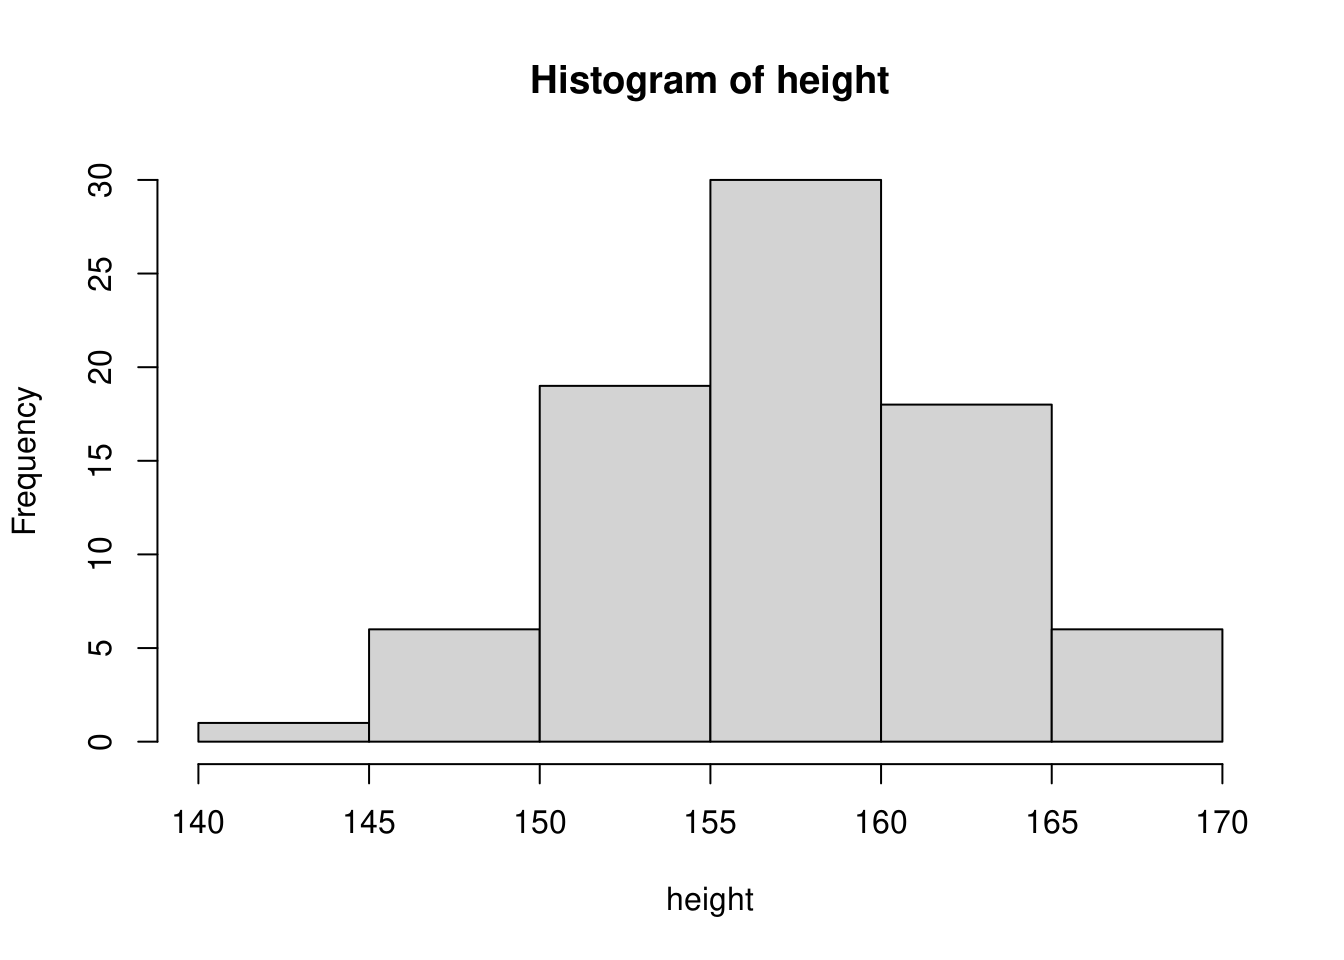
\includegraphics[width=0.9\linewidth,]{R_files/figure-latex/階級数をスタージェスの公式で求めた場合-1} \end{center}

 

\hypertarget{ux30b9ux30b3ux30c3ux30c8ux306eux9078ux629e}{%
\paragraph*{スコットの選択}\label{ux30b9ux30b3ux30c3ux30c8ux306eux9078ux629e}}
\addcontentsline{toc}{paragraph}{スコットの選択}

 スコットの選択は、データによってはスタージェスの公式と比べて階級数が少なくなる傾向があります。

\begin{Shaded}
\begin{Highlighting}[]
\FunctionTok{with}\NormalTok{(x, }\FunctionTok{hist}\NormalTok{(height, }\AttributeTok{breaks =} \StringTok{"Scott"}\NormalTok{))}
\end{Highlighting}
\end{Shaded}

\begin{center}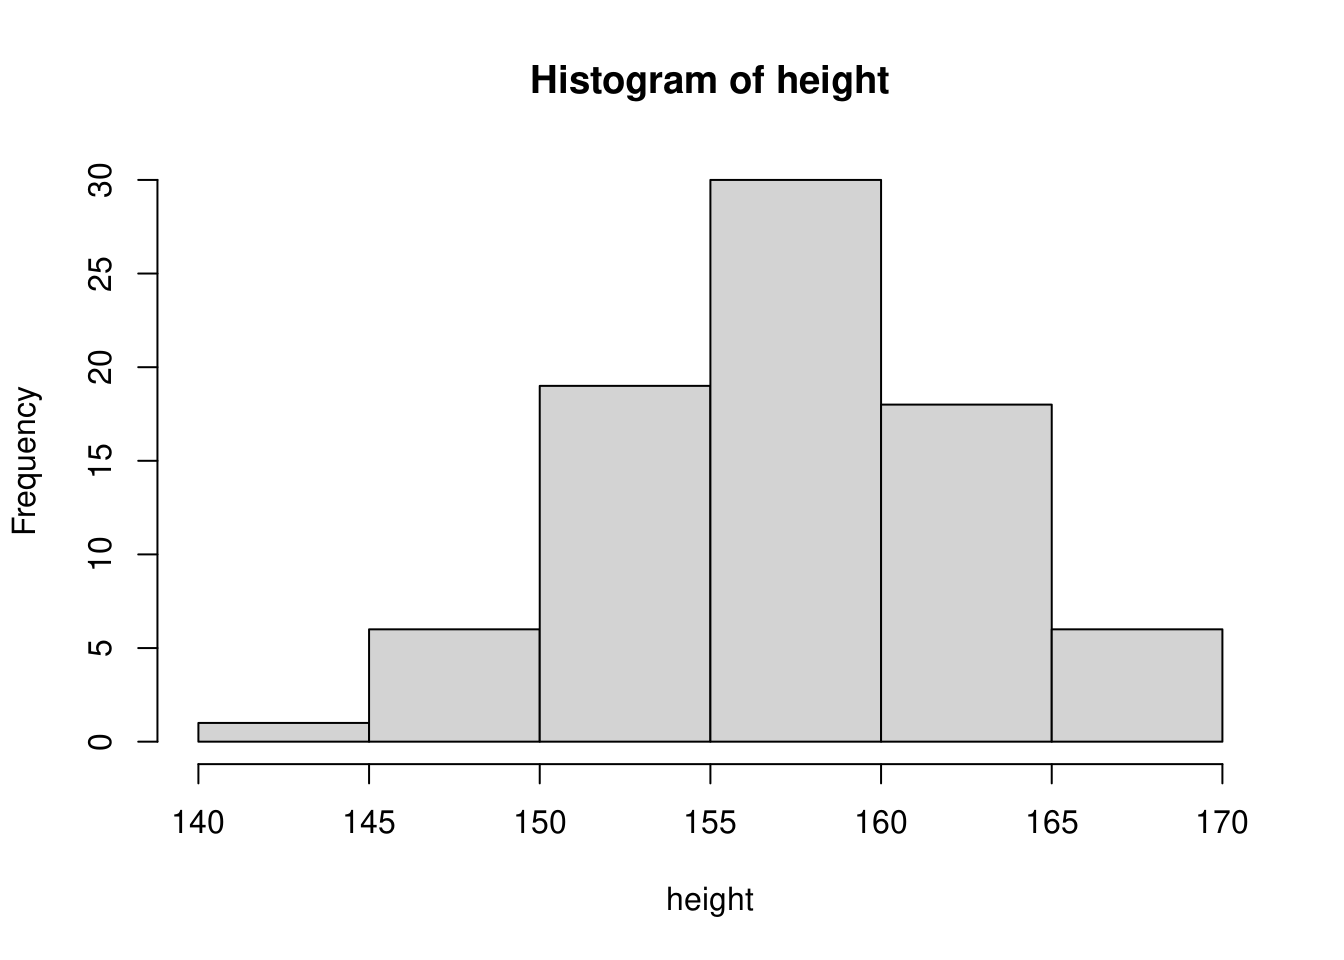
\includegraphics[width=0.9\linewidth,]{R_files/figure-latex/スコットの選択で求めた場合-1} \end{center}

 

\hypertarget{ux30d5ux30eaux30fcux30c9ux30deux30f3ux30c0ux30a4ux30a2ux30b3ux30cbux30b9ux306eux9078ux629e}{%
\paragraph*{フリードマン・ダイアコニスの選択}\label{ux30d5ux30eaux30fcux30c9ux30deux30f3ux30c0ux30a4ux30a2ux30b3ux30cbux30b9ux306eux9078ux629e}}
\addcontentsline{toc}{paragraph}{フリードマン・ダイアコニスの選択}

 フリードマン・ダイアコニスの法則とも呼ばれます。

\begin{Shaded}
\begin{Highlighting}[]
\FunctionTok{with}\NormalTok{(x, }\FunctionTok{hist}\NormalTok{(height, }\AttributeTok{breaks =} \StringTok{"FD"}\NormalTok{))}
\end{Highlighting}
\end{Shaded}

\begin{figure}[H]

{\centering 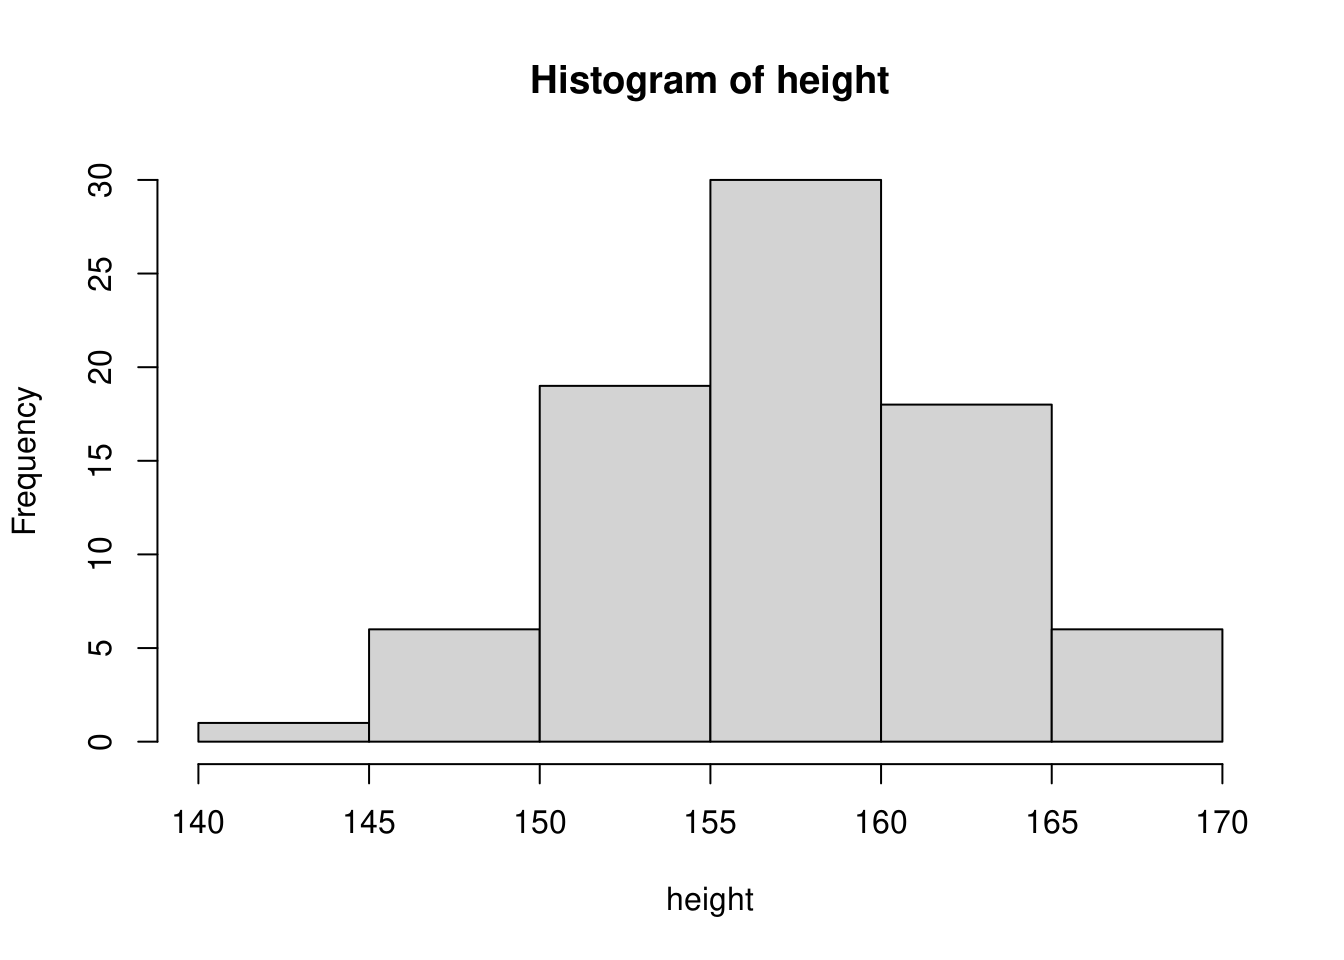
\includegraphics[width=0.9\linewidth,]{R_files/figure-latex/unnamed-chunk-26-1} 

}

\caption{階級をフリードマン・ダイアコニスの選択で求めた場合}\label{fig:unnamed-chunk-26}
\end{figure}

 

\hypertarget{ux968eux7d1aux306eux5883ux754cux306eux6271ux3044}{%
\subsection*{階級の境界の扱い}\label{ux968eux7d1aux306eux5883ux754cux306eux6271ux3044}}
\addcontentsline{toc}{subsection}{階級の境界の扱い}

 階級は下表のように「下端値〜上端値」の形式で表示されることが多いですが、\(140\)は階級に含まれるのか?\(145\)はどちらの階級に含まれるのか?を決めておかないと意図しない度数になってしまう場合があります。

\begin{longtable}[]{@{}lr@{}}
\toprule
階級 & 度数 \\
\midrule
\endhead
140〜145 & 1 \\
145〜150 & 6 \\
\ldots{} & \ldots{} \\
160〜165 & 16 \\
165〜170 & 6 \\
\bottomrule
\end{longtable}

 例えば、階級を「\(\mbox{下端値} < x \leq \mbox{上端値}\)」と定義した場合は、下図のようになります。

\begin{Shaded}
\begin{Highlighting}[]
\FunctionTok{with}\NormalTok{(x, }\FunctionTok{hist}\NormalTok{(height, }\AttributeTok{right =} \ConstantTok{TRUE}\NormalTok{))}
\end{Highlighting}
\end{Shaded}

\begin{figure}[H]

{\centering 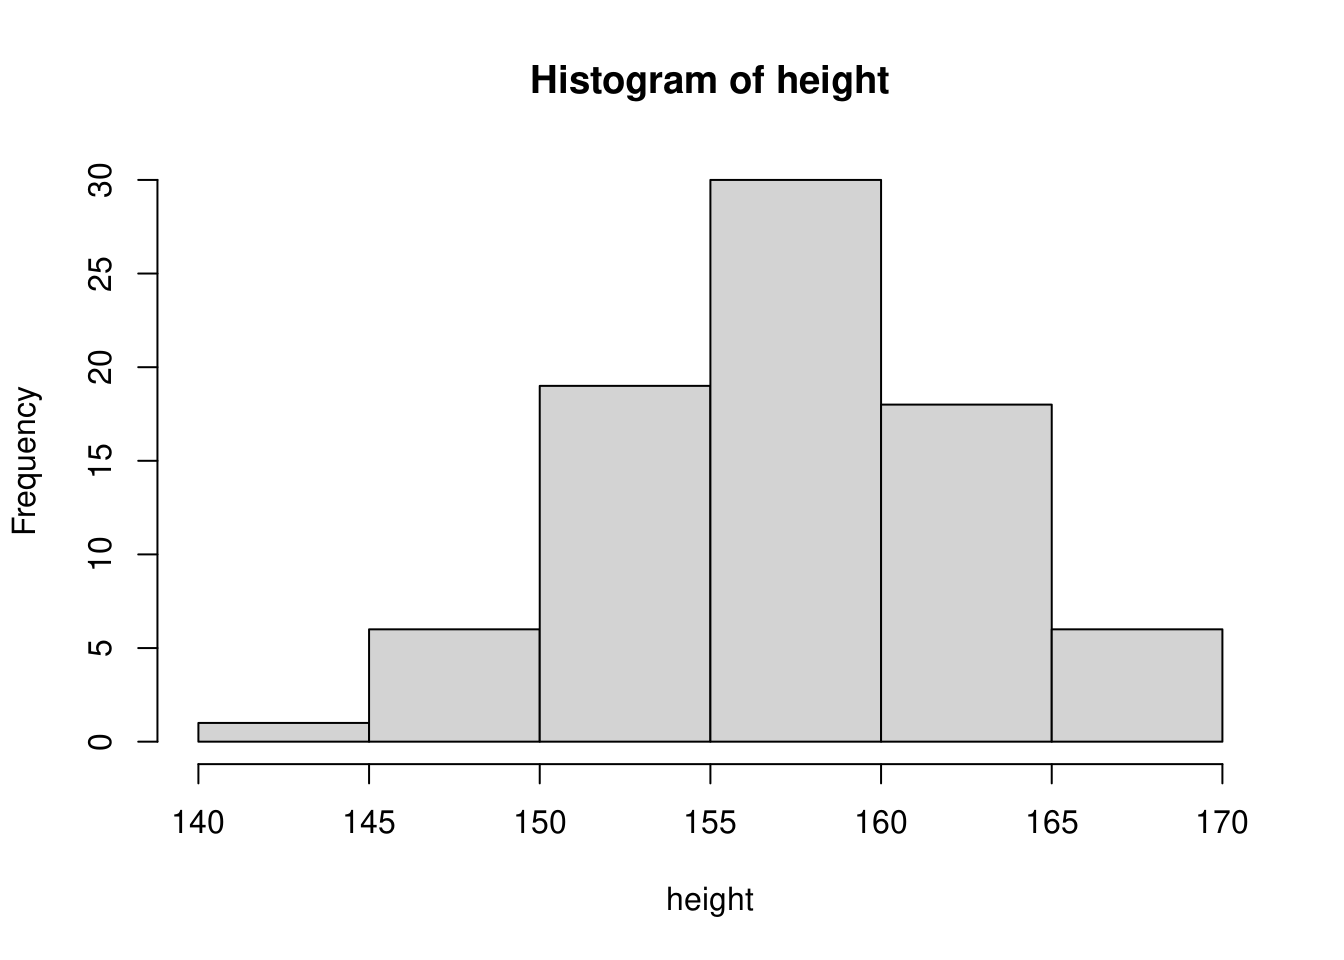
\includegraphics[width=0.9\linewidth,]{R_files/figure-latex/unnamed-chunk-27-1} 

}

\caption{上端を含める場合}\label{fig:unnamed-chunk-27}
\end{figure}

階級を「\(\mbox{下端値} \leq x <l \mbox{上端値}\)」と定義した場合は、分布形状が異なることが分かります。

\begin{Shaded}
\begin{Highlighting}[]
\FunctionTok{with}\NormalTok{(x, }\FunctionTok{hist}\NormalTok{(height, }\AttributeTok{right =} \ConstantTok{FALSE}\NormalTok{))}
\end{Highlighting}
\end{Shaded}

\begin{figure}[H]

{\centering 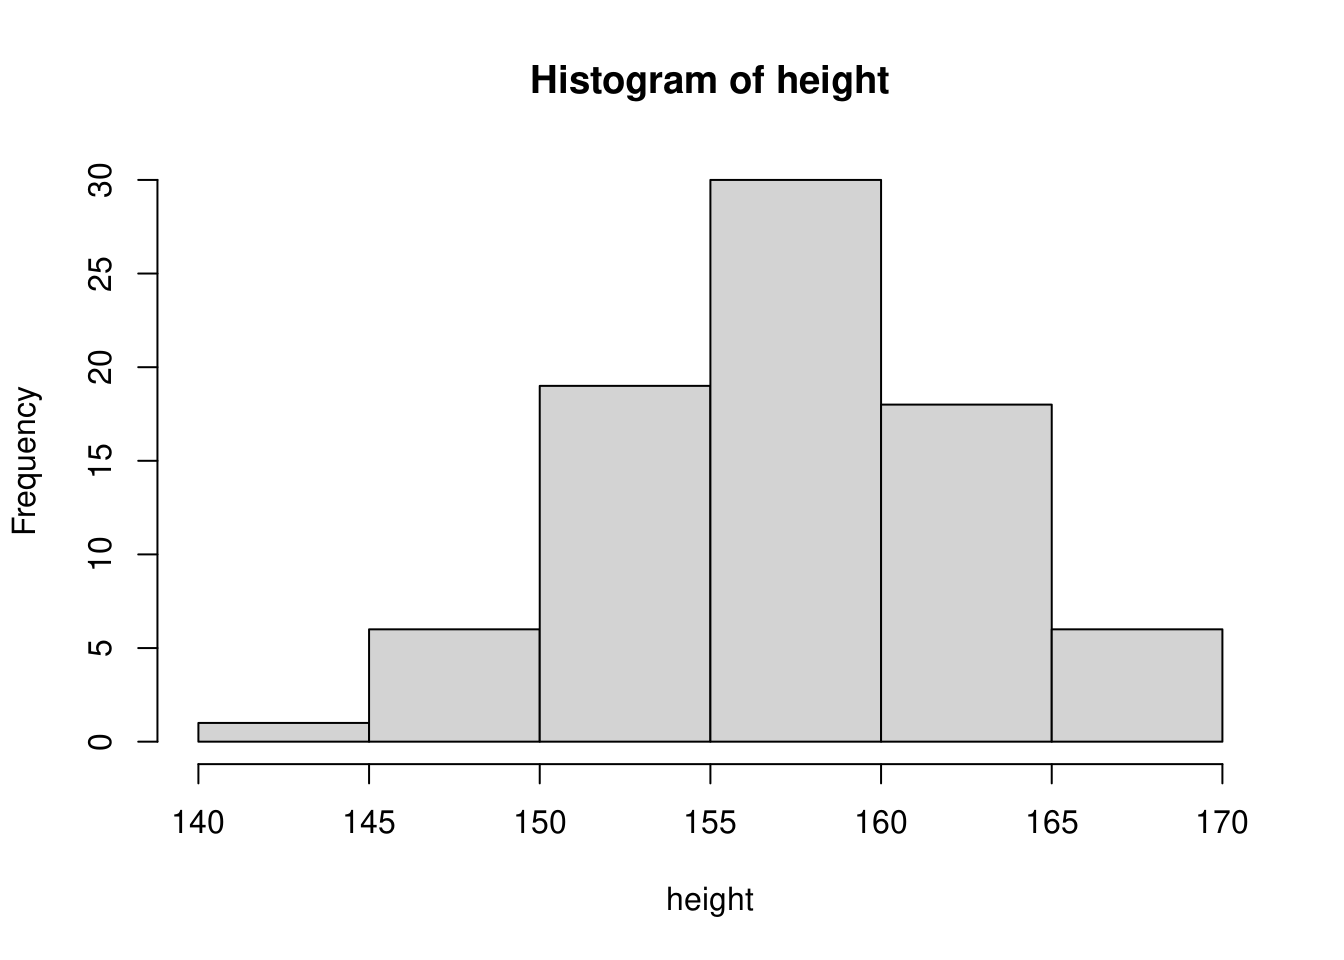
\includegraphics[width=0.9\linewidth,]{R_files/figure-latex/unnamed-chunk-28-1} 

}

\caption{下端を含める場合}\label{fig:unnamed-chunk-28}
\end{figure}

 このように階級によりヒストグラムの形状が変わってくる点には注意が必要です。なお、下端、上端の含め方を\href{https://k-metrics.netlify.app/post/2018-09/histogram/\#/\%E5\%B7\%A6\%E9\%96\%89\%E3\%81\%98\%E3\%81\%A8\%E5\%8F\%B3\%E9\%96\%89\%E3\%81\%98}{「左閉じ、右閉じ」と表現}することもあります。

 

\hypertarget{ux7b49ux9593ux9694ux3067ux306fux306aux3044ux968eux7d1a}{%
\section*{等間隔ではない階級}\label{ux7b49ux9593ux9694ux3067ux306fux306aux3044ux968eux7d1a}}
\addcontentsline{toc}{section}{等間隔ではない階級}

 度数分布表の階級は必ずしも等間隔である必要はありません。例えば、下図の世帯貯蓄のように度数の小さい階級をまとめたヒストグラムをしばしば見かけます。等間隔でないは階級は(最小値と最大値で桁が数桁異なるなど)幅が広いデータにおいて、階級を細かくしたい場合や等幅の階級でグラフ化するとデータを読み取りにくい場合などに使われます。

\begin{Shaded}
\begin{Highlighting}[]
\NormalTok{knitr}\SpecialCharTok{::}\FunctionTok{include\_graphics}\NormalTok{(}\StringTok{"https://www.stat.go.jp/naruhodo/img/picture/4\_8\_10.png"}\NormalTok{)}
\end{Highlighting}
\end{Shaded}

 このように階級幅が等間隔でない場合には、柱(棒)の面積が度数に対応するように高さを調整する必要があります。\\
 ヒストグラムは棒グラフとは異なり階級ごとの柱(棒)の面積が意味を持っています。高さは一般的に度数として表示されますが、密度として表示することもあります。高さ(密度)と幅(階級幅)を乗じたものが相対度数になります。相対度数は名前の通り度数に比例していますので、柱(棒)の面積が等しければ同じ度数ということを表します。\\
 \\
 例えば、テキストにある身長のデータの\(140cm\)から\(150cm\)をひとつの階級にまとめた場合、度数分布表は下表のようになります。

\begin{Shaded}
\begin{Highlighting}[]
\NormalTok{x }\SpecialCharTok{\%\textgreater{}\%} 
\NormalTok{  dplyr}\SpecialCharTok{::}\FunctionTok{mutate}\NormalTok{(}\AttributeTok{class =} \FunctionTok{cut}\NormalTok{(height,}
                            \AttributeTok{breaks =} \FunctionTok{c}\NormalTok{(}\DecValTok{140}\NormalTok{, }\DecValTok{150}\NormalTok{, }\DecValTok{155}\NormalTok{, }\DecValTok{160}\NormalTok{, }\DecValTok{165}\NormalTok{, }\DecValTok{170}\NormalTok{))) }\SpecialCharTok{\%\textgreater{}\%} 
\NormalTok{  dplyr}\SpecialCharTok{::}\FunctionTok{count}\NormalTok{(class) }\SpecialCharTok{\%\textgreater{}\%} 
\NormalTok{  dplyr}\SpecialCharTok{::}\FunctionTok{mutate}\NormalTok{(}\AttributeTok{prop =} \FunctionTok{prop.table}\NormalTok{(n)) }\SpecialCharTok{\%\textgreater{}\%} 
\NormalTok{  dplyr}\SpecialCharTok{::}\FunctionTok{rename}\NormalTok{(}\StringTok{\textasciigrave{}}\AttributeTok{階級}\StringTok{\textasciigrave{}} \OtherTok{=}\NormalTok{ class, }\StringTok{\textasciigrave{}}\AttributeTok{度数}\StringTok{\textasciigrave{}} \OtherTok{=}\NormalTok{ n, }\StringTok{\textasciigrave{}}\AttributeTok{相対度数}\StringTok{\textasciigrave{}} \OtherTok{=}\NormalTok{ prop)}
\end{Highlighting}
\end{Shaded}

\begin{verbatim}
## # A tibble: 5 x 3
##   階級       度数 相対度数
##   <fct>     <int>    <dbl>
## 1 (140,150]     7   0.0875
## 2 (150,155]    19   0.238 
## 3 (155,160]    30   0.375 
## 4 (160,165]    18   0.225 
## 5 (165,170]     6   0.075
\end{verbatim}

 これをヒストグラムとして描いた場合は、下図のようにならなければなりません。この図では縦軸は度数でなく密度になっています。

\begin{Shaded}
\begin{Highlighting}[]
\FunctionTok{with}\NormalTok{(x, }\FunctionTok{hist}\NormalTok{(height, }\AttributeTok{breaks =} \FunctionTok{c}\NormalTok{(}\DecValTok{140}\NormalTok{, }\DecValTok{150}\NormalTok{, }\DecValTok{155}\NormalTok{, }\DecValTok{160}\NormalTok{, }\DecValTok{165}\NormalTok{, }\DecValTok{170}\NormalTok{)))}
\end{Highlighting}
\end{Shaded}

\begin{figure}[H]

{\centering 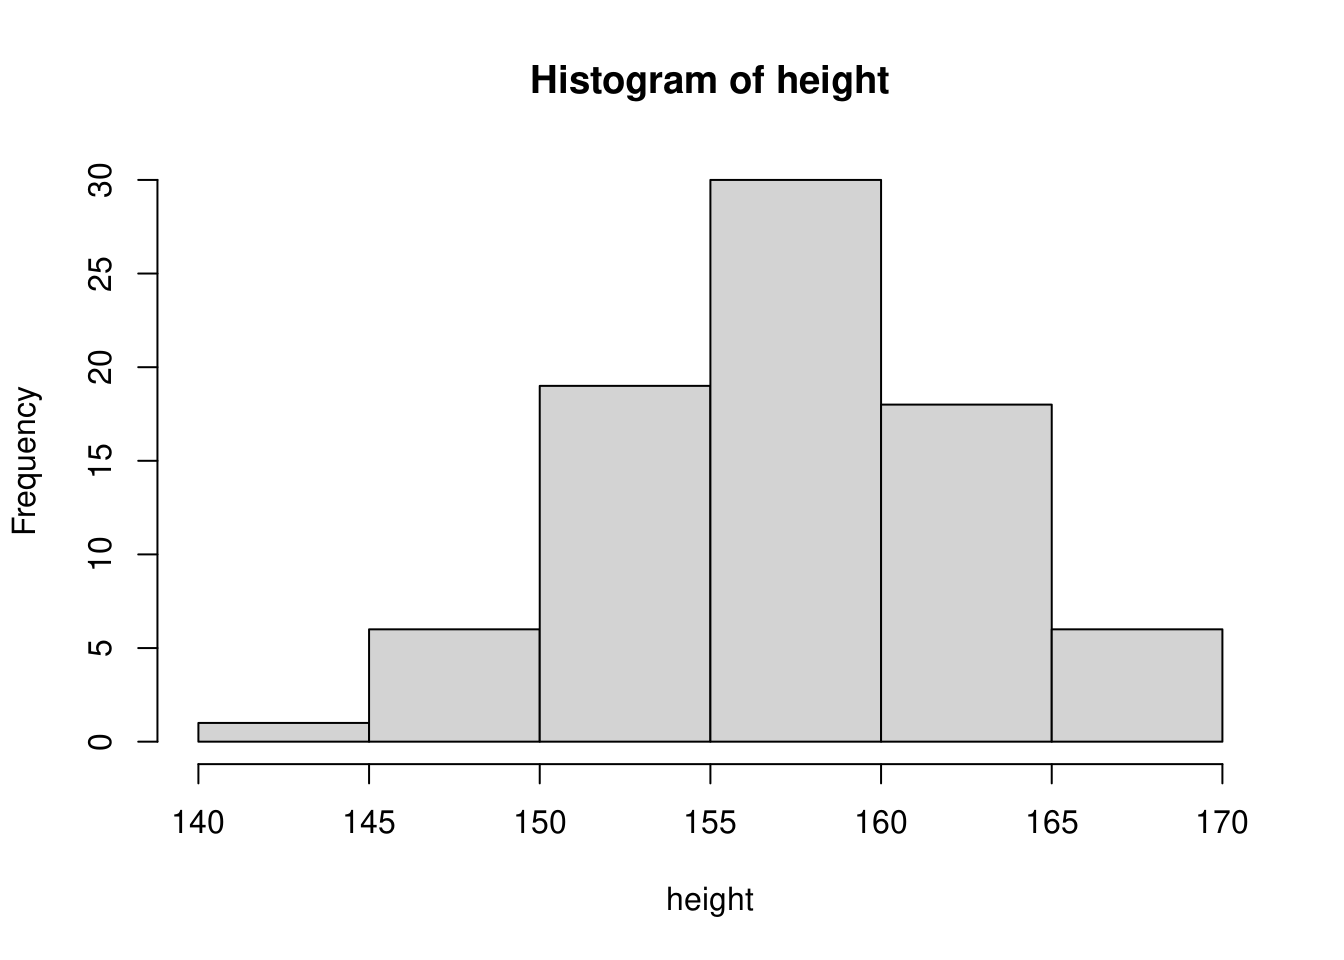
\includegraphics[width=0.9\linewidth,]{R_files/figure-latex/unnamed-chunk-31-1} 

}

\caption{正しいヒストグラム}\label{fig:unnamed-chunk-31}
\end{figure}

 密度(高さ)は左から\\
  0.00875, 0.0475, 0.075, 0.045, 0.015\\
 となっていますので、これに個々の階級幅(幅)\\
  10, 5, 5, 5, 5\\
 を乗じると個々の柱(棒)の面積は\\
  0.0875, 0.2375, 0.375, 0.225, 0.075\\
 となり、相対度数と等しいことがわかります。 

 度数を表示させるために下図のようなヒストグラムを描くことは好ましくありません。階級幅が等幅でない場合は度数分布表と共に密度のヒストグラムを示した方がよいでしょう。

\begin{Shaded}
\begin{Highlighting}[]
\FunctionTok{with}\NormalTok{(x, }\FunctionTok{hist}\NormalTok{(height, }\AttributeTok{breaks =} \FunctionTok{c}\NormalTok{(}\DecValTok{140}\NormalTok{, }\DecValTok{150}\NormalTok{, }\DecValTok{155}\NormalTok{, }\DecValTok{160}\NormalTok{, }\DecValTok{165}\NormalTok{, }\DecValTok{170}\NormalTok{), }\AttributeTok{freq =} \ConstantTok{TRUE}\NormalTok{))}
\end{Highlighting}
\end{Shaded}

\begin{figure}[H]

{\centering 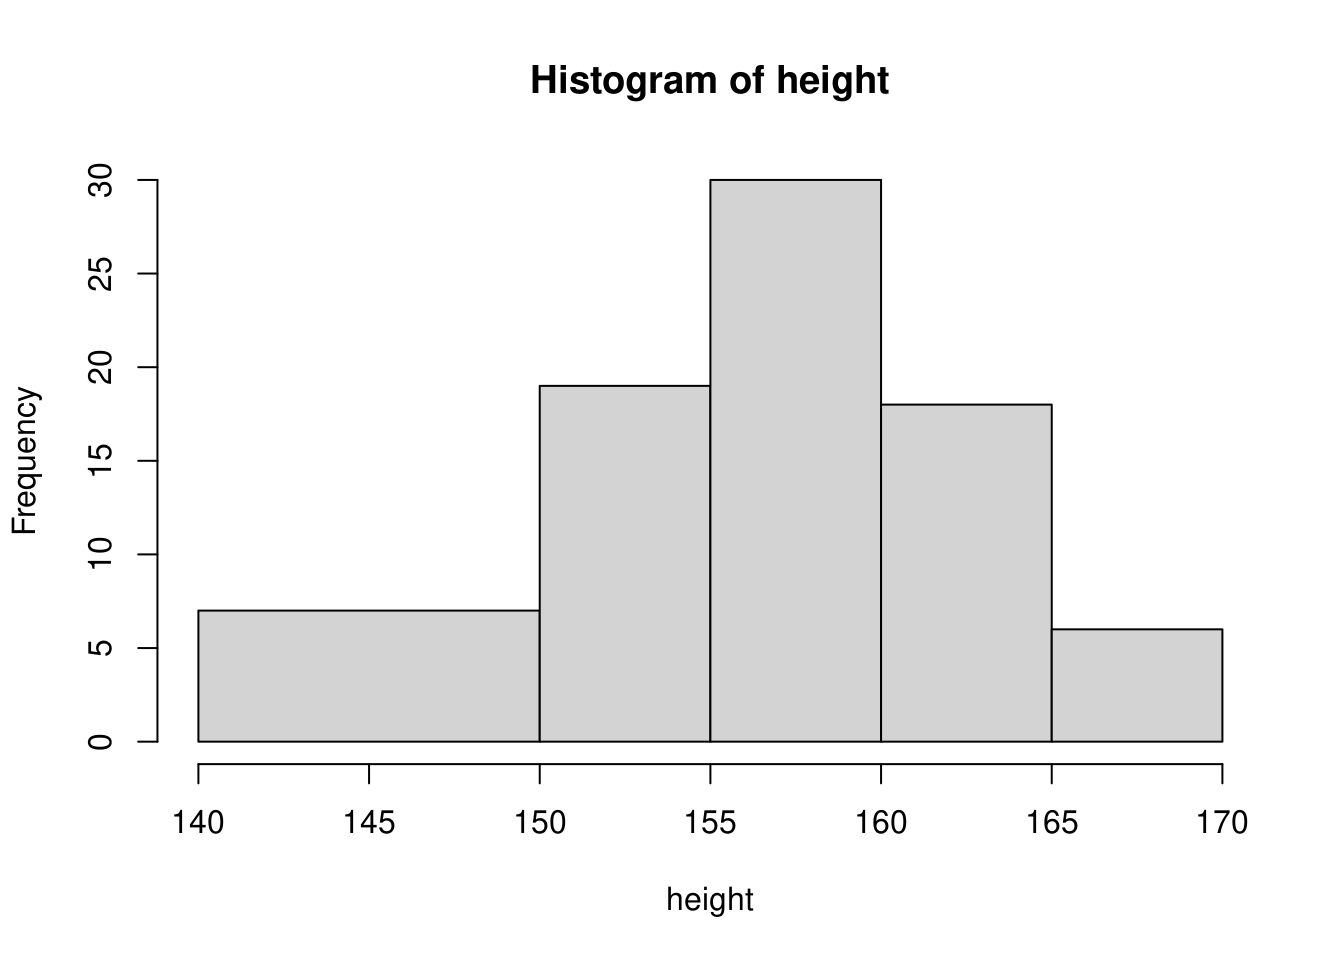
\includegraphics[width=0.9\linewidth,]{R_files/figure-latex/unnamed-chunk-33-1} 

}

\caption{好ましくないヒストグラム(単なる棒グラフ)}\label{fig:unnamed-chunk-33}
\end{figure}

\hypertarget{ux5e73ux5747ux5024ux3068ux306fux3084ux3058ux308dux3079ux3048ux306eux8996ux70b9ux3067ux3042ux308b}{%
\chapter{平均値とはやじろべえの視点である}\label{ux5e73ux5747ux5024ux3068ux306fux3084ux3058ux308dux3079ux3048ux306eux8996ux70b9ux3067ux3042ux308b}}

 本講では以下のデータフレームを利用しています。

\hypertarget{ux8eabux9577ux30c7ux30fcux30bf}{%
\subsubsection*{身長データ}\label{ux8eabux9577ux30c7ux30fcux30bf}}
\addcontentsline{toc}{subsubsection}{身長データ}

\begin{Shaded}
\begin{Highlighting}[]
\NormalTok{x}
\end{Highlighting}
\end{Shaded}

\begin{verbatim}
## # A tibble: 80 x 1
##    height
##     <dbl>
##  1    151
##  2    154
##  3    160
##  4    160
##  5    163
##  6    156
##  7    158
##  8    156
##  9    154
## 10    160
## # ... with 70 more rows
\end{verbatim}

\hypertarget{ux5ea6ux6570ux5206ux5e03ux8868}{%
\subsubsection*{度数分布表}\label{ux5ea6ux6570ux5206ux5e03ux8868}}
\addcontentsline{toc}{subsubsection}{度数分布表}

\begin{Shaded}
\begin{Highlighting}[]
\NormalTok{df}
\end{Highlighting}
\end{Shaded}

\begin{verbatim}
## # A tibble: 6 x 9
##   class         n     l     h  mids range cumsum_n   prop cumsum_prop
##   <fct>     <int> <dbl> <dbl> <dbl> <dbl>    <int>  <dbl>       <dbl>
## 1 (140,145]     1   140   145   143     5        1 0.0125      0.0125
## 2 (145,150]     6   145   150   148     5        7 0.075       0.0875
## 3 (150,155]    19   150   155   153     5       26 0.238       0.325 
## 4 (155,160]    30   155   160   158     5       56 0.375       0.7   
## 5 (160,165]    18   160   165   163     5       74 0.225       0.925 
## 6 (165,170]     6   165   170   168     5       80 0.075       1
\end{verbatim}

 

\hypertarget{ux7d71ux8a08ux91cfux306fux30c7ux30fcux30bfux3092ux8981ux7d04ux3059ux308bux6570ux5024}{%
\section{統計量は、データを要約する数値}\label{ux7d71ux8a08ux91cfux306fux30c7ux30fcux30bfux3092ux8981ux7d04ux3059ux308bux6570ux5024}}

 本稿で扱っている統計量(要約統計量)は平均のみです。

 

\hypertarget{ux5e73ux5747ux5024ux3068ux306f}{%
\section{平均値とは}\label{ux5e73ux5747ux5024ux3068ux306f}}

 本稿の平均値とは算術平均を意味しています。身長データ(\(x\))の平均値は157.575です。

 

\hypertarget{ux5ea6ux6570ux5206ux5e03ux8868ux3067ux306eux5e73ux5747ux5024}{%
\section{度数分布表での平均値}\label{ux5ea6ux6570ux5206ux5e03ux8868ux3067ux306eux5e73ux5747ux5024}}

\begin{Shaded}
\begin{Highlighting}[]
\NormalTok{df }\SpecialCharTok{\%\textgreater{}\%} 
\NormalTok{  dplyr}\SpecialCharTok{::}\FunctionTok{select}\NormalTok{(}\StringTok{\textasciigrave{}}\AttributeTok{階級}\StringTok{\textasciigrave{}} \OtherTok{=}\NormalTok{ class, }\StringTok{\textasciigrave{}}\AttributeTok{度数}\StringTok{\textasciigrave{}} \OtherTok{=}\NormalTok{ n, }\StringTok{\textasciigrave{}}\AttributeTok{階級値}\StringTok{\textasciigrave{}} \OtherTok{=}\NormalTok{ mids, }\StringTok{\textasciigrave{}}\AttributeTok{階級幅}\StringTok{\textasciigrave{}} \OtherTok{=}\NormalTok{ range,}
                \StringTok{\textasciigrave{}}\AttributeTok{累積度数}\StringTok{\textasciigrave{}} \OtherTok{=}\NormalTok{ cumsum\_n, }\StringTok{\textasciigrave{}}\AttributeTok{相対度数}\StringTok{\textasciigrave{}} \OtherTok{=}\NormalTok{ prop, }\StringTok{\textasciigrave{}}\AttributeTok{累積相対度数}\StringTok{\textasciigrave{}} \OtherTok{=}\NormalTok{ cumsum\_prop)}
\end{Highlighting}
\end{Shaded}

\begin{verbatim}
## # A tibble: 6 x 7
##   階級       度数 階級値 階級幅 累積度数 相対度数 累積相対度数
##   <fct>     <int>  <dbl>  <dbl>    <int>    <dbl>        <dbl>
## 1 (140,145]     1    143      5        1   0.0125       0.0125
## 2 (145,150]     6    148      5        7   0.075        0.0875
## 3 (150,155]    19    153      5       26   0.238        0.325 
## 4 (155,160]    30    158      5       56   0.375        0.7   
## 5 (160,165]    18    163      5       74   0.225        0.925 
## 6 (165,170]     6    168      5       80   0.075        1
\end{verbatim}

 (算術)平均は全ての観測値の総和を総データ数で除したものですので、観測値を各階級の代表値である階級値で近似すると下式が成り立つことが分かります。

\[\mbox{平均} = \frac{\sum{\mbox{観測値}_i}}{総データ数} = \frac{\sum{\mbox{観測値}_i}}{\sum{度数}_i} \fallingdotseq \frac{\sum{(\mbox{階級値}_i \times \mbox{度数}_i)}}{\sum{度数}_i} = \sum{(\mbox{階級値}_i \times \mbox{相対度数}_i)}\]

 なぜなら \[\frac{\mbox{度数}_i}{\sum{\mbox{度数}_i}} = \mbox{相対度数}_i\]

\[i = 1, 2, ... , n\]

\begin{Shaded}
\begin{Highlighting}[]
\NormalTok{df }\SpecialCharTok{\%\textgreater{}\%} 
\NormalTok{  dplyr}\SpecialCharTok{::}\FunctionTok{select}\NormalTok{(}\AttributeTok{A =}\NormalTok{ mids, }\AttributeTok{B =}\NormalTok{ prop) }\SpecialCharTok{\%\textgreater{}\%} 
\NormalTok{  dplyr}\SpecialCharTok{::}\FunctionTok{mutate}\NormalTok{(}\StringTok{\textasciigrave{}}\AttributeTok{A x B}\StringTok{\textasciigrave{}} \OtherTok{=}\NormalTok{ A }\SpecialCharTok{*}\NormalTok{ B) }\SpecialCharTok{\%\textgreater{}\%} 
\NormalTok{  dplyr}\SpecialCharTok{::}\FunctionTok{rename}\NormalTok{(}\StringTok{\textasciigrave{}}\AttributeTok{A 階級値}\StringTok{\textasciigrave{}} \OtherTok{=}\NormalTok{ A, }\StringTok{\textasciigrave{}}\AttributeTok{B 相対度数}\StringTok{\textasciigrave{}} \OtherTok{=}\NormalTok{ B, }\StringTok{\textasciigrave{}}\AttributeTok{A x B}\StringTok{\textasciigrave{}} \OtherTok{=} \StringTok{\textasciigrave{}}\AttributeTok{A x B}\StringTok{\textasciigrave{}}\NormalTok{)}
\end{Highlighting}
\end{Shaded}

\begin{verbatim}
## # A tibble: 6 x 3
##   `A 階級値` `B 相対度数` `A x B`
##        <dbl>        <dbl>   <dbl>
## 1        143       0.0125    1.79
## 2        148       0.075    11.1 
## 3        153       0.238    36.3 
## 4        158       0.375    59.2 
## 5        163       0.225    36.7 
## 6        168       0.075    12.6
\end{verbatim}

\begin{Shaded}
\begin{Highlighting}[]
\NormalTok{df }\SpecialCharTok{\%\textgreater{}\%} 
\NormalTok{  dplyr}\SpecialCharTok{::}\FunctionTok{select}\NormalTok{(}\AttributeTok{A =}\NormalTok{ mids, }\AttributeTok{B =}\NormalTok{ prop) }\SpecialCharTok{\%\textgreater{}\%} 
\NormalTok{  dplyr}\SpecialCharTok{::}\FunctionTok{mutate}\NormalTok{(}\StringTok{\textasciigrave{}}\AttributeTok{A x B}\StringTok{\textasciigrave{}} \OtherTok{=}\NormalTok{ A }\SpecialCharTok{*}\NormalTok{ B) }\SpecialCharTok{\%\textgreater{}\%} 
\NormalTok{  dplyr}\SpecialCharTok{::}\FunctionTok{summarise}\NormalTok{(}\StringTok{\textasciigrave{}}\AttributeTok{平均値}\StringTok{\textasciigrave{}} \OtherTok{=} \FunctionTok{sum}\NormalTok{(}\StringTok{\textasciigrave{}}\AttributeTok{A x B}\StringTok{\textasciigrave{}}\NormalTok{))}
\end{Highlighting}
\end{Shaded}

\begin{verbatim}
## # A tibble: 1 x 1
##   平均値
##    <dbl>
## 1   158.
\end{verbatim}

 実データで求めた平均値は157.575ですので、階級値から求めた平均値との差は-0.175となり、度数分布表を作ることは平均値に大きな影響を与えないことが分かります。

 

\hypertarget{ux5e73ux5747ux5024ux306eux30d2ux30b9ux30c8ux30b0ux30e9ux30e0ux306eux4e2dux3067ux306eux5f79ux5272}{%
\section{平均値のヒストグラムの中での役割}\label{ux5e73ux5747ux5024ux306eux30d2ux30b9ux30c8ux30b0ux30e9ux30e0ux306eux4e2dux3067ux306eux5f79ux5272}}

 階級値から求めた平均値をヒストグラム上にプロットすると下図のようになります。

\begin{Shaded}
\begin{Highlighting}[]
\FunctionTok{with}\NormalTok{(x, }\FunctionTok{hist}\NormalTok{(height))}
\FunctionTok{abline}\NormalTok{(}\AttributeTok{v =} \FloatTok{157.75}\NormalTok{, }\AttributeTok{lty =} \DecValTok{2}\NormalTok{)}
\end{Highlighting}
\end{Shaded}

\begin{center}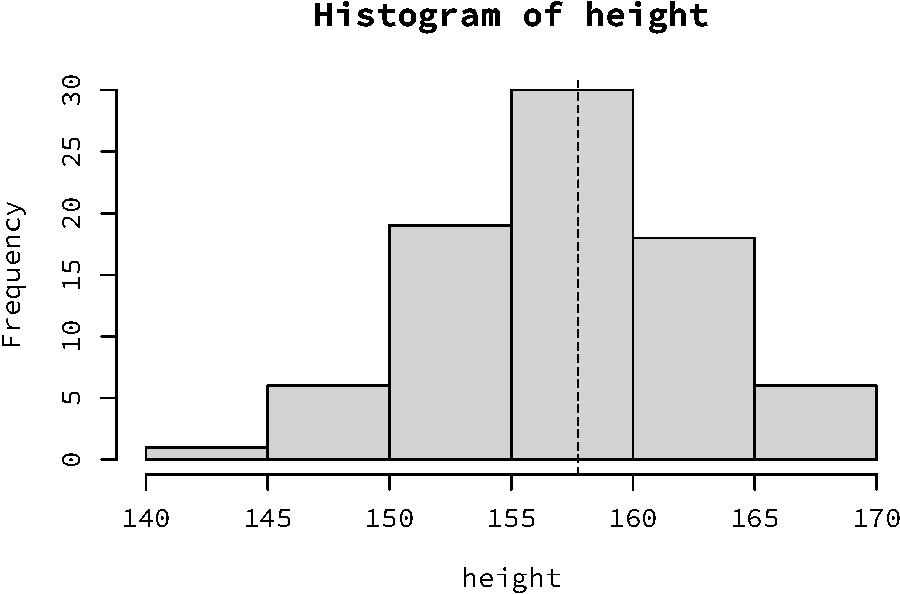
\includegraphics[width=0.9\linewidth,]{R_files/figure-latex/unnamed-chunk-39-1} \end{center}

 

\hypertarget{ux5e73ux5747ux5024ux3092ux3069ux3046ux6349ux3048ux308bux3079ux304dux304b}{%
\section{平均値をどう捉えるべきか}\label{ux5e73ux5747ux5024ux3092ux3069ux3046ux6349ux3048ux308bux3079ux304dux304b}}

 平均値の捉え方は様々考えられますが、テキストでは下記のようにまとめています。

\begin{itemize}
\tightlist
\item
  全データ(値)を代表する値(点)
\item
  データは平均値の周辺に分布する
\item
  数多く現れるデータは平均値への影響が大きい
\item
  データの分布が対象の場合、平均値は対象軸
\end{itemize}

 

\hypertarget{ux7df4ux7fd2ux554fux984c-1}{%
\section{練習問題}\label{ux7df4ux7fd2ux554fux984c-1}}

\hypertarget{ux89e3ux7b54ux4f8b-1}{%
\subsection{解答例}\label{ux89e3ux7b54ux4f8b-1}}

\begin{Shaded}
\begin{Highlighting}[]
\FunctionTok{data.frame}\NormalTok{(}\AttributeTok{mids =} \FunctionTok{c}\NormalTok{(}\DecValTok{30}\NormalTok{, }\DecValTok{50}\NormalTok{, }\DecValTok{70}\NormalTok{, }\DecValTok{90}\NormalTok{, }\DecValTok{110}\NormalTok{, }\DecValTok{130}\NormalTok{), }\AttributeTok{n =} \FunctionTok{c}\NormalTok{(}\DecValTok{5}\NormalTok{, }\DecValTok{10}\NormalTok{, }\DecValTok{15}\NormalTok{, }\DecValTok{40}\NormalTok{, }\DecValTok{20}\NormalTok{, }\DecValTok{10}\NormalTok{)) }\SpecialCharTok{\%\textgreater{}\%} 
\NormalTok{  dplyr}\SpecialCharTok{::}\FunctionTok{mutate}\NormalTok{(}\AttributeTok{prop =} \FunctionTok{prop.table}\NormalTok{(n), }\AttributeTok{cm =}\NormalTok{ mids }\SpecialCharTok{*}\NormalTok{ prop) }\SpecialCharTok{\%\textgreater{}\%} 
\NormalTok{  dplyr}\SpecialCharTok{::}\FunctionTok{rename}\NormalTok{(}\StringTok{\textasciigrave{}}\AttributeTok{階級値}\StringTok{\textasciigrave{}} \OtherTok{=}\NormalTok{ mids, }\StringTok{\textasciigrave{}}\AttributeTok{度数}\StringTok{\textasciigrave{}} \OtherTok{=}\NormalTok{ n, }\StringTok{\textasciigrave{}}\AttributeTok{相対度数}\StringTok{\textasciigrave{}} \OtherTok{=}\NormalTok{ prop, }\StringTok{\textasciigrave{}}\AttributeTok{階級値×相対度数}\StringTok{\textasciigrave{}} \OtherTok{=}\NormalTok{ cm)}
\end{Highlighting}
\end{Shaded}

\begin{verbatim}
##   階級値 度数 相対度数 階級値×相対度数
## 1     30    5     0.05              1.5
## 2     50   10     0.10              5.0
## 3     70   15     0.15             10.5
## 4     90   40     0.40             36.0
## 5    110   20     0.20             22.0
## 6    130   10     0.10             13.0
\end{verbatim}

\begin{Shaded}
\begin{Highlighting}[]
\FunctionTok{data.frame}\NormalTok{(}\AttributeTok{mids =} \FunctionTok{c}\NormalTok{(}\DecValTok{30}\NormalTok{, }\DecValTok{50}\NormalTok{, }\DecValTok{70}\NormalTok{, }\DecValTok{90}\NormalTok{, }\DecValTok{110}\NormalTok{, }\DecValTok{130}\NormalTok{), }\AttributeTok{n =} \FunctionTok{c}\NormalTok{(}\DecValTok{5}\NormalTok{, }\DecValTok{10}\NormalTok{, }\DecValTok{15}\NormalTok{, }\DecValTok{40}\NormalTok{, }\DecValTok{20}\NormalTok{, }\DecValTok{10}\NormalTok{)) }\SpecialCharTok{\%\textgreater{}\%} 
\NormalTok{  dplyr}\SpecialCharTok{::}\FunctionTok{mutate}\NormalTok{(}\AttributeTok{prop =} \FunctionTok{prop.table}\NormalTok{(n), }\AttributeTok{cm =}\NormalTok{ mids }\SpecialCharTok{*}\NormalTok{ prop) }\SpecialCharTok{\%\textgreater{}\%} 
\NormalTok{  dplyr}\SpecialCharTok{::}\FunctionTok{summarise}\NormalTok{(}\StringTok{\textasciigrave{}}\AttributeTok{平均値}\StringTok{\textasciigrave{}} \OtherTok{=} \FunctionTok{sum}\NormalTok{(cm))}
\end{Highlighting}
\end{Shaded}

\begin{verbatim}
##   平均値
## 1     88
\end{verbatim}

\hypertarget{ux30b3ux30e9ux30e0ux5e73ux5747ux5024ux306eux3068ux308aux65b9ux306fuxff11ux3064ux3067ux306fux306aux3044}{%
\section*{【コラム】平均値のとり方は、1つではない}\label{ux30b3ux30e9ux30e0ux5e73ux5747ux5024ux306eux3068ux308aux65b9ux306fuxff11ux3064ux3067ux306fux306aux3044}}
\addcontentsline{toc}{section}{【コラム】平均値のとり方は、1つではない}

\hypertarget{ux7b97ux8853ux5e73ux5747arithmetic-mean}{%
\subsection*{算術平均(Arithmetic Mean)}\label{ux7b97ux8853ux5e73ux5747arithmetic-mean}}
\addcontentsline{toc}{subsection}{算術平均(Arithmetic Mean)}

\[\frac{\sum_{i=1}^n{x_i}}{n}\]

\begin{Shaded}
\begin{Highlighting}[]
\FunctionTok{sum}\NormalTok{(}\FunctionTok{c}\NormalTok{(}\DecValTok{10}\NormalTok{, }\DecValTok{90}\NormalTok{)) }\SpecialCharTok{/} \FunctionTok{length}\NormalTok{(}\FunctionTok{c}\NormalTok{(}\DecValTok{10}\NormalTok{, }\DecValTok{90}\NormalTok{))}
\end{Highlighting}
\end{Shaded}

\begin{verbatim}
## [1] 50
\end{verbatim}

\begin{Shaded}
\begin{Highlighting}[]
\FunctionTok{mean}\NormalTok{(}\FunctionTok{c}\NormalTok{(}\DecValTok{10}\NormalTok{, }\DecValTok{90}\NormalTok{))}
\end{Highlighting}
\end{Shaded}

\begin{verbatim}
## [1] 50
\end{verbatim}

 

\hypertarget{ux5e7eux4f55ux5e73ux5747geometric-meanux307eux305fux306fux76f8ux4e57ux5e73ux5747}{%
\subsection*{幾何平均(Geometric Mean)または相乗平均}\label{ux5e7eux4f55ux5e73ux5747geometric-meanux307eux305fux306fux76f8ux4e57ux5e73ux5747}}
\addcontentsline{toc}{subsection}{幾何平均(Geometric Mean)または相乗平均}

\[\sqrt{\prod_{i=1}^n{x_i}}\]

\begin{Shaded}
\begin{Highlighting}[]
\NormalTok{psych}\SpecialCharTok{::}\FunctionTok{geometric.mean}\NormalTok{(}\FunctionTok{c}\NormalTok{(}\DecValTok{10}\NormalTok{, }\DecValTok{90}\NormalTok{))}
\end{Highlighting}
\end{Shaded}

\begin{verbatim}
## [1] 30
\end{verbatim}

 

\hypertarget{ux4e8cux4e57ux5e73ux5747root-mean-square}{%
\subsection*{二乗平均(Root Mean Square)}\label{ux4e8cux4e57ux5e73ux5747root-mean-square}}
\addcontentsline{toc}{subsection}{二乗平均(Root Mean Square)}

\[\sqrt{\frac{\sum_{i=1}^n{x_i^2}}{n}}\]

\begin{Shaded}
\begin{Highlighting}[]
\FunctionTok{sqrt}\NormalTok{(}\FunctionTok{mean}\NormalTok{(}\FunctionTok{c}\NormalTok{(}\DecValTok{10}\NormalTok{, }\DecValTok{90}\NormalTok{) }\SpecialCharTok{\^{}} \DecValTok{2}\NormalTok{))}
\end{Highlighting}
\end{Shaded}

\begin{verbatim}
## [1] 64.03124
\end{verbatim}

 

\hypertarget{ux8abfux548cux5e73ux5747harmonic-mean}{%
\subsection*{調和平均(Harmonic Mean)}\label{ux8abfux548cux5e73ux5747harmonic-mean}}
\addcontentsline{toc}{subsection}{調和平均(Harmonic Mean)}

\[\frac{n}{\sum_{i=1}^n{\frac{1}{x_i}}}\]

\begin{Shaded}
\begin{Highlighting}[]
\NormalTok{psych}\SpecialCharTok{::}\FunctionTok{harmonic.mean}\NormalTok{(}\FunctionTok{c}\NormalTok{(}\DecValTok{10}\NormalTok{, }\DecValTok{90}\NormalTok{))}
\end{Highlighting}
\end{Shaded}

\begin{verbatim}
## [1] 18
\end{verbatim}

 

\hypertarget{ux30c8ux30eaux30e0ux5e73ux5747}{%
\subsection*{トリム平均}\label{ux30c8ux30eaux30e0ux5e73ux5747}}
\addcontentsline{toc}{subsection}{トリム平均}

 トリム平均は体操競技の評点などで使われる平均値の計算方法で、値を小さい方から順に並べ、上位側と下位側から一定の割合で値を除き算術平均を求めます。外れ値や異常値などを影響を排除するために使われることが多いです。

\begin{Shaded}
\begin{Highlighting}[]
\FunctionTok{mean}\NormalTok{(}\FunctionTok{c}\NormalTok{(}\DecValTok{0}\NormalTok{, }\DecValTok{1}\SpecialCharTok{:}\DecValTok{8}\NormalTok{, }\DecValTok{30}\NormalTok{))}
\end{Highlighting}
\end{Shaded}

\begin{verbatim}
## [1] 6.6
\end{verbatim}

\begin{Shaded}
\begin{Highlighting}[]
\FunctionTok{mean}\NormalTok{(}\FunctionTok{c}\NormalTok{(}\DecValTok{0}\NormalTok{, }\DecValTok{1}\SpecialCharTok{:}\DecValTok{8}\NormalTok{, }\DecValTok{30}\NormalTok{), }\AttributeTok{trim =} \FloatTok{0.25}\NormalTok{)  }\CommentTok{\# データの両側2.5\%を対象外とする}
\end{Highlighting}
\end{Shaded}

\begin{verbatim}
## [1] 4.5
\end{verbatim}

 

\hypertarget{ux8ffdux52a0ux554fux984c}{%
\section*{追加問題}\label{ux8ffdux52a0ux554fux984c}}
\addcontentsline{toc}{section}{追加問題}

 身長のデータを用いて階級幅が変わると度数分布表から求める平均値がどのように変化するか確認してみましょう。

\hypertarget{ux968eux7d1aux5e45ux304cux500dux306bux306aux3063ux305fux5834ux5408}{%
\subsection*{階級幅が倍になった場合}\label{ux968eux7d1aux5e45ux304cux500dux306bux306aux3063ux305fux5834ux5408}}
\addcontentsline{toc}{subsection}{階級幅が倍になった場合}

\begin{Shaded}
\begin{Highlighting}[]
\NormalTok{x }\SpecialCharTok{\%\textgreater{}\%} 
\NormalTok{  dplyr}\SpecialCharTok{::}\FunctionTok{mutate}\NormalTok{(}\AttributeTok{class =} \FunctionTok{cut}\NormalTok{(height,}
                            \AttributeTok{breaks =} \FunctionTok{c}\NormalTok{(}\DecValTok{140}\NormalTok{, }\DecValTok{150}\NormalTok{, }\DecValTok{160}\NormalTok{, }\DecValTok{170}\NormalTok{),}
                            \AttributeTok{include.lowest =} \ConstantTok{FALSE}\NormalTok{, }\AttributeTok{right =} \ConstantTok{TRUE}\NormalTok{)) }\SpecialCharTok{\%\textgreater{}\%} 
\NormalTok{  dplyr}\SpecialCharTok{::}\FunctionTok{count}\NormalTok{(class) }\SpecialCharTok{\%\textgreater{}\%} 
\NormalTok{  dplyr}\SpecialCharTok{::}\FunctionTok{mutate}\NormalTok{(}\AttributeTok{class\_value =} \FunctionTok{as.character}\NormalTok{(class)) }\SpecialCharTok{\%\textgreater{}\%} 
\NormalTok{  tidyr}\SpecialCharTok{::}\FunctionTok{separate}\NormalTok{(class\_value, }\AttributeTok{into =} \FunctionTok{c}\NormalTok{(}\StringTok{"l"}\NormalTok{, }\StringTok{"h"}\NormalTok{), }\AttributeTok{sep =} \StringTok{","}\NormalTok{) }\SpecialCharTok{\%\textgreater{}\%} 
\NormalTok{  dplyr}\SpecialCharTok{::}\FunctionTok{mutate}\NormalTok{(}\AttributeTok{l =} \FunctionTok{as.numeric}\NormalTok{(stringr}\SpecialCharTok{::}\FunctionTok{str\_remove}\NormalTok{(l, }\StringTok{"[[:punct:]]"}\NormalTok{)),}
                \AttributeTok{h =} \FunctionTok{as.numeric}\NormalTok{(stringr}\SpecialCharTok{::}\FunctionTok{str\_remove}\NormalTok{(h, }\StringTok{"[[:punct:]]"}\NormalTok{))) }\SpecialCharTok{\%\textgreater{}\%} 
\NormalTok{  dplyr}\SpecialCharTok{::}\FunctionTok{mutate}\NormalTok{(}\AttributeTok{mids =}\NormalTok{ ((l }\SpecialCharTok{+} \DecValTok{1}\NormalTok{) }\SpecialCharTok{+}\NormalTok{ h) }\SpecialCharTok{/} \DecValTok{2}\NormalTok{) }\SpecialCharTok{\%\textgreater{}\%} 
\NormalTok{  dplyr}\SpecialCharTok{::}\FunctionTok{mutate}\NormalTok{(}\AttributeTok{range =}\NormalTok{ h }\SpecialCharTok{{-}}\NormalTok{ l, }\AttributeTok{cumsum\_n =} \FunctionTok{cumsum}\NormalTok{(n),}
                \AttributeTok{prop =} \FunctionTok{prop.table}\NormalTok{(n), }\AttributeTok{cumsum\_prop =} \FunctionTok{cumsum}\NormalTok{(prop)) }\SpecialCharTok{\%\textgreater{}\%} 
\NormalTok{  dplyr}\SpecialCharTok{::}\FunctionTok{select}\NormalTok{(}\AttributeTok{A =}\NormalTok{ mids, }\AttributeTok{B =}\NormalTok{ prop) }\SpecialCharTok{\%\textgreater{}\%} 
\NormalTok{  dplyr}\SpecialCharTok{::}\FunctionTok{mutate}\NormalTok{(}\StringTok{\textasciigrave{}}\AttributeTok{A x B}\StringTok{\textasciigrave{}} \OtherTok{=}\NormalTok{ A }\SpecialCharTok{*}\NormalTok{ B) }\SpecialCharTok{\%\textgreater{}\%} 
\NormalTok{  dplyr}\SpecialCharTok{::}\FunctionTok{summarise}\NormalTok{(}\StringTok{\textasciigrave{}}\AttributeTok{階級値による平均値}\StringTok{\textasciigrave{}} \OtherTok{=} \FunctionTok{sum}\NormalTok{(}\StringTok{\textasciigrave{}}\AttributeTok{A x B}\StringTok{\textasciigrave{}}\NormalTok{)) }\SpecialCharTok{\%\textgreater{}\%} 
\NormalTok{  dplyr}\SpecialCharTok{::}\FunctionTok{mutate}\NormalTok{(}\StringTok{\textasciigrave{}}\AttributeTok{算術平均}\StringTok{\textasciigrave{}} \OtherTok{=} \FunctionTok{mean}\NormalTok{(x}\SpecialCharTok{$}\NormalTok{height), }\StringTok{\textasciigrave{}}\AttributeTok{差}\StringTok{\textasciigrave{}} \OtherTok{=} \StringTok{\textasciigrave{}}\AttributeTok{算術平均}\StringTok{\textasciigrave{}} \SpecialCharTok{{-}} \StringTok{\textasciigrave{}}\AttributeTok{階級値による平均値}\StringTok{\textasciigrave{}}\NormalTok{)}
\end{Highlighting}
\end{Shaded}

\begin{verbatim}
## # A tibble: 1 x 3
##   階級値による平均値 算術平均      差
##                <dbl>    <dbl>   <dbl>
## 1               158.     158. -0.0500
\end{verbatim}

\hypertarget{ux968eux7d1aux5e45ux304cux534aux5206ux306bux306aux3063ux305fux5834ux5408}{%
\subsection*{階級幅が半分になった場合}\label{ux968eux7d1aux5e45ux304cux534aux5206ux306bux306aux3063ux305fux5834ux5408}}
\addcontentsline{toc}{subsection}{階級幅が半分になった場合}

\begin{Shaded}
\begin{Highlighting}[]
\NormalTok{x }\SpecialCharTok{\%\textgreater{}\%} 
\NormalTok{  dplyr}\SpecialCharTok{::}\FunctionTok{mutate}\NormalTok{(}\AttributeTok{class =} \FunctionTok{cut}\NormalTok{(height,}
                            \AttributeTok{breaks =} \FunctionTok{seq}\NormalTok{(}\AttributeTok{from =} \DecValTok{140}\NormalTok{, }\AttributeTok{to =} \DecValTok{170}\NormalTok{, }\AttributeTok{by =} \FloatTok{2.5}\NormalTok{),}
                            \AttributeTok{include.lowest =} \ConstantTok{FALSE}\NormalTok{, }\AttributeTok{right =} \ConstantTok{TRUE}\NormalTok{)) }\SpecialCharTok{\%\textgreater{}\%} 
\NormalTok{  dplyr}\SpecialCharTok{::}\FunctionTok{count}\NormalTok{(class) }\SpecialCharTok{\%\textgreater{}\%} 
\NormalTok{  dplyr}\SpecialCharTok{::}\FunctionTok{mutate}\NormalTok{(}\AttributeTok{class\_value =} \FunctionTok{as.character}\NormalTok{(class)) }\SpecialCharTok{\%\textgreater{}\%} 
\NormalTok{  tidyr}\SpecialCharTok{::}\FunctionTok{separate}\NormalTok{(class\_value, }\AttributeTok{into =} \FunctionTok{c}\NormalTok{(}\StringTok{"l"}\NormalTok{, }\StringTok{"h"}\NormalTok{), }\AttributeTok{sep =} \StringTok{","}\NormalTok{) }\SpecialCharTok{\%\textgreater{}\%} 
\NormalTok{  dplyr}\SpecialCharTok{::}\FunctionTok{mutate}\NormalTok{(}\AttributeTok{l =} \FunctionTok{as.numeric}\NormalTok{(stringr}\SpecialCharTok{::}\FunctionTok{str\_remove}\NormalTok{(l, }\StringTok{"[[:punct:]]"}\NormalTok{)),}
                \AttributeTok{h =} \FunctionTok{as.numeric}\NormalTok{(stringr}\SpecialCharTok{::}\FunctionTok{str\_remove}\NormalTok{(h, }\StringTok{"[[:punct:]]"}\NormalTok{))) }\SpecialCharTok{\%\textgreater{}\%} 
\NormalTok{  dplyr}\SpecialCharTok{::}\FunctionTok{mutate}\NormalTok{(}\AttributeTok{mids =}\NormalTok{ ((l }\SpecialCharTok{+} \DecValTok{1}\NormalTok{) }\SpecialCharTok{+}\NormalTok{ h) }\SpecialCharTok{/} \DecValTok{2}\NormalTok{) }\SpecialCharTok{\%\textgreater{}\%} 
\NormalTok{  dplyr}\SpecialCharTok{::}\FunctionTok{mutate}\NormalTok{(}\AttributeTok{range =}\NormalTok{ h }\SpecialCharTok{{-}}\NormalTok{ l, }\AttributeTok{cumsum\_n =} \FunctionTok{cumsum}\NormalTok{(n),}
                \AttributeTok{prop =} \FunctionTok{prop.table}\NormalTok{(n), }\AttributeTok{cumsum\_prop =} \FunctionTok{cumsum}\NormalTok{(prop)) }\SpecialCharTok{\%\textgreater{}\%} 
\NormalTok{  dplyr}\SpecialCharTok{::}\FunctionTok{select}\NormalTok{(}\AttributeTok{A =}\NormalTok{ mids, }\AttributeTok{B =}\NormalTok{ prop) }\SpecialCharTok{\%\textgreater{}\%} 
\NormalTok{  dplyr}\SpecialCharTok{::}\FunctionTok{mutate}\NormalTok{(}\StringTok{\textasciigrave{}}\AttributeTok{A x B}\StringTok{\textasciigrave{}} \OtherTok{=}\NormalTok{ A }\SpecialCharTok{*}\NormalTok{ B) }\SpecialCharTok{\%\textgreater{}\%} 
\NormalTok{  dplyr}\SpecialCharTok{::}\FunctionTok{summarise}\NormalTok{(}\StringTok{\textasciigrave{}}\AttributeTok{階級値による平均値}\StringTok{\textasciigrave{}} \OtherTok{=} \FunctionTok{sum}\NormalTok{(}\StringTok{\textasciigrave{}}\AttributeTok{A x B}\StringTok{\textasciigrave{}}\NormalTok{)) }\SpecialCharTok{\%\textgreater{}\%} 
\NormalTok{  dplyr}\SpecialCharTok{::}\FunctionTok{mutate}\NormalTok{(}\StringTok{\textasciigrave{}}\AttributeTok{算術平均}\StringTok{\textasciigrave{}} \OtherTok{=} \FunctionTok{mean}\NormalTok{(x}\SpecialCharTok{$}\NormalTok{height), }\StringTok{\textasciigrave{}}\AttributeTok{差}\StringTok{\textasciigrave{}} \OtherTok{=} \StringTok{\textasciigrave{}}\AttributeTok{算術平均}\StringTok{\textasciigrave{}} \SpecialCharTok{{-}} \StringTok{\textasciigrave{}}\AttributeTok{階級値による平均値}\StringTok{\textasciigrave{}}\NormalTok{)}
\end{Highlighting}
\end{Shaded}

\begin{verbatim}
## # A tibble: 1 x 3
##   階級値による平均値 算術平均     差
##                <dbl>    <dbl>  <dbl>
## 1               158.     158. -0.281
\end{verbatim}

\hypertarget{ux30c7ux30fcux30bfux306eux6563ux3089ux3070ux308aux5177ux5408ux3092ux898bux7a4dux3082ux308bux7d71ux8a08ux91cf}{%
\chapter{データの散らばり具合を見積もる統計量}\label{ux30c7ux30fcux30bfux306eux6563ux3089ux3070ux308aux5177ux5408ux3092ux898bux7a4dux3082ux308bux7d71ux8a08ux91cf}}

\hypertarget{ux30c7ux30fcux30bfux306eux6563ux3089ux3070ux308aux3084ux30d0ux30e9ux30c4ux30adux3092ux77e5ux308aux305fux3044}{%
\section{データの散らばりやバラツキを知りたい}\label{ux30c7ux30fcux30bfux306eux6563ux3089ux3070ux308aux3084ux30d0ux30e9ux30c4ux30adux3092ux77e5ux308aux305fux3044}}

 第2講で学んだ平均値(算術平均)は、データを代表する統計量で、ある一点(支点・重心)を示しているに過ぎません。データが平均値の周辺にどのように分布しているかはヒストグラムを使うことで視覚的には確認できますが、統計量として数値的に扱えた方がなにかと便利なはずです。

 

\hypertarget{ux30d0ux30b9ux306eux5230ux7740ux6642ux523bux306eux4f8bux3067ux5206ux6563ux3092ux7406ux89e3ux3059ux308b}{%
\section{バスの到着時刻の例で分散を理解する}\label{ux30d0ux30b9ux306eux5230ux7740ux6642ux523bux306eux4f8bux3067ux5206ux6563ux3092ux7406ux89e3ux3059ux308b}}

 蛇足ですが実際の路線バスでは予定時刻より早く到着しないように調整運転がなされていますので、時刻より大幅に早着することは稀です。

\begin{Shaded}
\begin{Highlighting}[]
\NormalTok{x }\OtherTok{\textless{}{-}} \FunctionTok{scan}\NormalTok{(}\AttributeTok{file =} \StringTok{"../data/P36\_図表3{-}1.csv"}\NormalTok{, }\AttributeTok{sep =} \StringTok{","}\NormalTok{)}
\NormalTok{x}
\end{Highlighting}
\end{Shaded}

\begin{verbatim}
## [1] 32 27 29 34 33
\end{verbatim}

 平均値を求める\texttt{mean()}関数がありますが、ここでは平均値の計算式通りの計算を行っています。

\begin{Shaded}
\begin{Highlighting}[]
\StringTok{\textasciigrave{}}\AttributeTok{平均値}\StringTok{\textasciigrave{}} \OtherTok{\textless{}{-}} \FunctionTok{sum}\NormalTok{(x) }\SpecialCharTok{/} \FunctionTok{length}\NormalTok{(x)}
\StringTok{\textasciigrave{}}\AttributeTok{平均値}\StringTok{\textasciigrave{}}
\end{Highlighting}
\end{Shaded}

\begin{verbatim}
## [1] 31
\end{verbatim}

\begin{Shaded}
\begin{Highlighting}[]
\StringTok{\textasciigrave{}}\AttributeTok{偏差}\StringTok{\textasciigrave{}} \OtherTok{=}\NormalTok{ x }\SpecialCharTok{{-}} \StringTok{\textasciigrave{}}\AttributeTok{平均値}\StringTok{\textasciigrave{}}
\StringTok{\textasciigrave{}}\AttributeTok{偏差}\StringTok{\textasciigrave{}}
\end{Highlighting}
\end{Shaded}

\begin{verbatim}
## [1]  1 -4 -2  3  2
\end{verbatim}

 偏差の総和は必ずゼロ(\(0\))になります。

\begin{Shaded}
\begin{Highlighting}[]
\FunctionTok{sum}\NormalTok{(}\StringTok{\textasciigrave{}}\AttributeTok{偏差}\StringTok{\textasciigrave{}}\NormalTok{)}
\end{Highlighting}
\end{Shaded}

\begin{verbatim}
## [1] 0
\end{verbatim}

 偏差の二乗和をデータの個数で割ったものは、(標本)分散と呼ばれます。不偏分散と呼ばれる分散は計算式が異なります。Rで分散を計算する\texttt{var()}関数は不偏分散を求める関数です。

\begin{Shaded}
\begin{Highlighting}[]
\FunctionTok{sum}\NormalTok{(}\StringTok{\textasciigrave{}}\AttributeTok{偏差}\StringTok{\textasciigrave{}} \SpecialCharTok{\^{}} \DecValTok{2}\NormalTok{) }\SpecialCharTok{/} \FunctionTok{length}\NormalTok{(x)}
\end{Highlighting}
\end{Shaded}

\begin{verbatim}
## [1] 6.8
\end{verbatim}

 偏差の二乗平均値(\(= \sqrt{\mbox{分散}}\))は標準偏差と呼ばれます。Rで標準偏差を計算する\texttt{sd()}関数は不偏分散のルートを取ったものです。

\begin{Shaded}
\begin{Highlighting}[]
\FunctionTok{sqrt}\NormalTok{(}\FunctionTok{sum}\NormalTok{(}\StringTok{\textasciigrave{}}\AttributeTok{偏差}\StringTok{\textasciigrave{}} \SpecialCharTok{\^{}} \DecValTok{2}\NormalTok{) }\SpecialCharTok{/} \FunctionTok{length}\NormalTok{(x))}
\end{Highlighting}
\end{Shaded}

\begin{verbatim}
## [1] 2.607681
\end{verbatim}

 

\hypertarget{ux6a19ux6e96ux504fux5deeux306eux610fux5473}{%
\section{標準偏差の意味}\label{ux6a19ux6e96ux504fux5deeux306eux610fux5473}}

\begin{Shaded}
\begin{Highlighting}[]
\NormalTok{x }\OtherTok{\textless{}{-}} \FunctionTok{read.csv}\NormalTok{(}\AttributeTok{file =} \StringTok{"../data/P39\_図表3{-}4.csv"}\NormalTok{) }
\NormalTok{x}
\end{Highlighting}
\end{Shaded}

\begin{verbatim}
##   X Y
## 1 4 1
## 2 4 2
## 3 5 6
## 4 6 7
## 5 6 9
\end{verbatim}

x

\begin{Shaded}
\begin{Highlighting}[]
\NormalTok{mean }\OtherTok{\textless{}{-}}\NormalTok{ x }\SpecialCharTok{\%\textgreater{}\%} 
\NormalTok{  dplyr}\SpecialCharTok{::}\FunctionTok{summarise}\NormalTok{(}\StringTok{\textasciigrave{}}\AttributeTok{X平均値}\StringTok{\textasciigrave{}} \OtherTok{=} \FunctionTok{mean}\NormalTok{(X), }\StringTok{\textasciigrave{}}\AttributeTok{Y平均値}\StringTok{\textasciigrave{}} \OtherTok{=} \FunctionTok{mean}\NormalTok{(Y))}
\NormalTok{mean}
\end{Highlighting}
\end{Shaded}

\begin{verbatim}
##   X平均値 Y平均値
## 1       5       5
\end{verbatim}

\begin{Shaded}
\begin{Highlighting}[]
\NormalTok{x }\SpecialCharTok{\%\textgreater{}\%} 
\NormalTok{  dplyr}\SpecialCharTok{::}\FunctionTok{mutate}\NormalTok{(}\StringTok{\textasciigrave{}}\AttributeTok{X偏差}\StringTok{\textasciigrave{}} \OtherTok{=}\NormalTok{ X }\SpecialCharTok{{-}}\NormalTok{ mean}\SpecialCharTok{$}\StringTok{\textasciigrave{}}\AttributeTok{X平均値}\StringTok{\textasciigrave{}}\NormalTok{, }\StringTok{\textasciigrave{}}\AttributeTok{Y偏差}\StringTok{\textasciigrave{}} \OtherTok{=}\NormalTok{ Y }\SpecialCharTok{{-}}\NormalTok{ mean}\SpecialCharTok{$}\StringTok{\textasciigrave{}}\AttributeTok{Y平均値}\StringTok{\textasciigrave{}}\NormalTok{)}
\end{Highlighting}
\end{Shaded}

\begin{verbatim}
##   X Y X偏差 Y偏差
## 1 4 1    -1    -4
## 2 4 2    -1    -3
## 3 5 6     0     1
## 4 6 7     1     2
## 5 6 9     1     4
\end{verbatim}

\begin{Shaded}
\begin{Highlighting}[]
\NormalTok{x }\SpecialCharTok{\%\textgreater{}\%} 
\NormalTok{  dplyr}\SpecialCharTok{::}\FunctionTok{mutate}\NormalTok{(}\StringTok{\textasciigrave{}}\AttributeTok{X偏差}\StringTok{\textasciigrave{}} \OtherTok{=}\NormalTok{ X }\SpecialCharTok{{-}}\NormalTok{ mean}\SpecialCharTok{$}\StringTok{\textasciigrave{}}\AttributeTok{X平均値}\StringTok{\textasciigrave{}}\NormalTok{, }\StringTok{\textasciigrave{}}\AttributeTok{Y偏差}\StringTok{\textasciigrave{}} \OtherTok{=}\NormalTok{ Y }\SpecialCharTok{{-}}\NormalTok{ mean}\SpecialCharTok{$}\StringTok{\textasciigrave{}}\AttributeTok{Y平均値}\StringTok{\textasciigrave{}}\NormalTok{) }\SpecialCharTok{\%\textgreater{}\%} 
\NormalTok{  dplyr}\SpecialCharTok{::}\FunctionTok{summarise}\NormalTok{(}\StringTok{\textasciigrave{}}\AttributeTok{X標準偏差}\StringTok{\textasciigrave{}} \OtherTok{=} \FunctionTok{sqrt}\NormalTok{(}\FunctionTok{sum}\NormalTok{(}\StringTok{\textasciigrave{}}\AttributeTok{X偏差}\StringTok{\textasciigrave{}} \SpecialCharTok{\^{}} \DecValTok{2}\NormalTok{) }\SpecialCharTok{/} \FunctionTok{length}\NormalTok{(X)),}
                   \StringTok{\textasciigrave{}}\AttributeTok{Y標準偏差}\StringTok{\textasciigrave{}} \OtherTok{=} \FunctionTok{sqrt}\NormalTok{(}\FunctionTok{sum}\NormalTok{(}\StringTok{\textasciigrave{}}\AttributeTok{Y偏差}\StringTok{\textasciigrave{}} \SpecialCharTok{\^{}} \DecValTok{2}\NormalTok{) }\SpecialCharTok{/} \FunctionTok{length}\NormalTok{(Y)))}
\end{Highlighting}
\end{Shaded}

\begin{verbatim}
##   X標準偏差 Y標準偏差
## 1 0.8944272   3.03315
\end{verbatim}

 偏差と標準偏差を可視化すると下図のようになり、XよりYの方が広範囲に分布していることが分かります。

\begin{Shaded}
\begin{Highlighting}[]
\NormalTok{x }\SpecialCharTok{\%\textgreater{}\%} 
\NormalTok{  dplyr}\SpecialCharTok{::}\FunctionTok{mutate}\NormalTok{(}\StringTok{\textasciigrave{}}\AttributeTok{X偏差}\StringTok{\textasciigrave{}} \OtherTok{=}\NormalTok{ X }\SpecialCharTok{{-}}\NormalTok{ mean}\SpecialCharTok{$}\StringTok{\textasciigrave{}}\AttributeTok{X平均値}\StringTok{\textasciigrave{}}\NormalTok{, }\StringTok{\textasciigrave{}}\AttributeTok{Y偏差}\StringTok{\textasciigrave{}} \OtherTok{=}\NormalTok{ Y }\SpecialCharTok{{-}}\NormalTok{ mean}\SpecialCharTok{$}\StringTok{\textasciigrave{}}\AttributeTok{Y平均値}\StringTok{\textasciigrave{}}\NormalTok{) }\SpecialCharTok{\%\textgreater{}\%} 
\NormalTok{  dplyr}\SpecialCharTok{::}\FunctionTok{select}\NormalTok{(}\SpecialCharTok{{-}}\NormalTok{X, }\SpecialCharTok{{-}}\NormalTok{Y) }\SpecialCharTok{\%\textgreater{}\%} 
  \FunctionTok{stripchart}\NormalTok{(}\AttributeTok{xlim =} \FunctionTok{c}\NormalTok{(}\SpecialCharTok{{-}}\DecValTok{5}\NormalTok{, }\DecValTok{5}\NormalTok{))}
\FunctionTok{abline}\NormalTok{(}\AttributeTok{v =} \FunctionTok{c}\NormalTok{(}\SpecialCharTok{{-}}\FloatTok{0.89}\NormalTok{, }\FloatTok{0.89}\NormalTok{), }\AttributeTok{lty =} \DecValTok{3}\NormalTok{)  }\CommentTok{\# X標準偏差/ドット(点線)}
\FunctionTok{abline}\NormalTok{(}\AttributeTok{v =} \FunctionTok{c}\NormalTok{(}\SpecialCharTok{{-}}\FloatTok{3.03}\NormalTok{, }\FloatTok{3.03}\NormalTok{), }\AttributeTok{lty =} \DecValTok{2}\NormalTok{)  }\CommentTok{\# Y標準偏差/ダッシュ(鎖線)}
\end{Highlighting}
\end{Shaded}

\begin{center}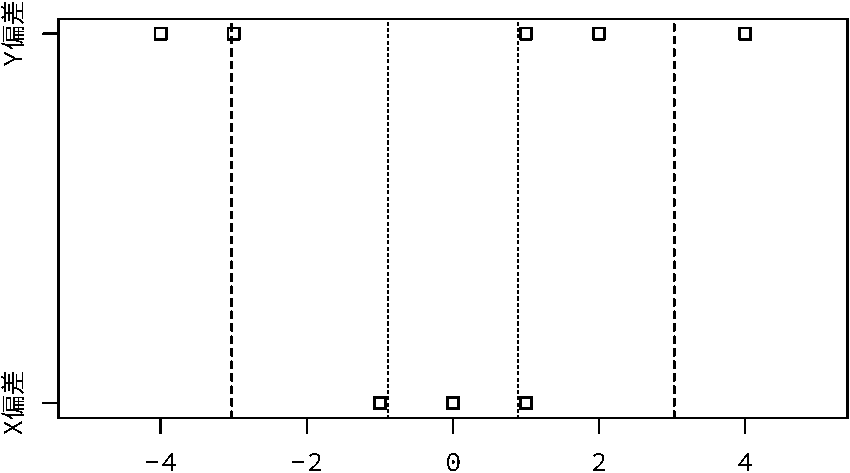
\includegraphics[width=0.9\linewidth,]{R_files/figure-latex/unnamed-chunk-60-1} \end{center}

\hypertarget{ux5ea6ux6570ux5206ux5e03ux8868ux304bux3089ux6a19ux6e96ux504fux5deeux3092ux6c42ux3081ux308b}{%
\section{度数分布表から標準偏差を求める}\label{ux5ea6ux6570ux5206ux5e03ux8868ux304bux3089ux6a19ux6e96ux504fux5deeux3092ux6c42ux3081ux308b}}

\begin{Shaded}
\begin{Highlighting}[]
\NormalTok{x }\OtherTok{\textless{}{-}} \FunctionTok{read.csv}\NormalTok{(}\AttributeTok{file =} \StringTok{"../data/P40\_図表3{-}6.csv"}\NormalTok{, }\AttributeTok{fileEncoding =} \StringTok{"UTF{-}8"}\NormalTok{)}
\NormalTok{x}
\end{Highlighting}
\end{Shaded}

\begin{verbatim}
##   A階級値 B相対度数
## 1       1       0.3
## 2       2       0.5
## 3       3       0.1
## 4       4       0.1
\end{verbatim}

 第2講の「2−3 度数分布表での平均値」で学んだように度数分布表から平均値(の近似値)は \[\mbox{平均値} \fallingdotseq \sum{(\mbox{階級値} \times \mbox{相対度数})}\]  で求めることができます。

\begin{Shaded}
\begin{Highlighting}[]
\NormalTok{x }\SpecialCharTok{\%\textgreater{}\%} 
\NormalTok{  dplyr}\SpecialCharTok{::}\FunctionTok{mutate}\NormalTok{(}\StringTok{\textasciigrave{}}\AttributeTok{AxB}\StringTok{\textasciigrave{}} \OtherTok{=} \StringTok{\textasciigrave{}}\AttributeTok{A階級値}\StringTok{\textasciigrave{}} \SpecialCharTok{*} \StringTok{\textasciigrave{}}\AttributeTok{B相対度数}\StringTok{\textasciigrave{}}\NormalTok{)}
\end{Highlighting}
\end{Shaded}

\begin{verbatim}
##   A階級値 B相対度数 AxB
## 1       1       0.3 0.3
## 2       2       0.5 1.0
## 3       3       0.1 0.3
## 4       4       0.1 0.4
\end{verbatim}

\begin{Shaded}
\begin{Highlighting}[]
\StringTok{\textasciigrave{}}\AttributeTok{平均値}\StringTok{\textasciigrave{}} \OtherTok{\textless{}{-}}\NormalTok{ x }\SpecialCharTok{\%\textgreater{}\%} 
\NormalTok{  dplyr}\SpecialCharTok{::}\FunctionTok{mutate}\NormalTok{(}\StringTok{\textasciigrave{}}\AttributeTok{AxB}\StringTok{\textasciigrave{}} \OtherTok{=} \StringTok{\textasciigrave{}}\AttributeTok{A階級値}\StringTok{\textasciigrave{}} \SpecialCharTok{*} \StringTok{\textasciigrave{}}\AttributeTok{B相対度数}\StringTok{\textasciigrave{}}\NormalTok{) }\SpecialCharTok{\%\textgreater{}\%} 
\NormalTok{  dplyr}\SpecialCharTok{::}\FunctionTok{summarize}\NormalTok{(}\StringTok{\textasciigrave{}}\AttributeTok{平均値}\StringTok{\textasciigrave{}} \OtherTok{=} \FunctionTok{sum}\NormalTok{(}\StringTok{\textasciigrave{}}\AttributeTok{AxB}\StringTok{\textasciigrave{}}\NormalTok{)) }\SpecialCharTok{\%\textgreater{}\%} 
\NormalTok{  dplyr}\SpecialCharTok{::}\FunctionTok{pull}\NormalTok{(}\StringTok{\textasciigrave{}}\AttributeTok{平均値}\StringTok{\textasciigrave{}}\NormalTok{)}
\StringTok{\textasciigrave{}}\AttributeTok{平均値}\StringTok{\textasciigrave{}}
\end{Highlighting}
\end{Shaded}

\begin{verbatim}
## [1] 2
\end{verbatim}

 平均値を求められたので \[\mbox{階級の偏差(C階級値-平均値)} = \mbox{階級値} - \mbox{平均値}\]  とすると度数分布表の計算値と同じ考え方を適用し \[\mbox{階級の偏差の二乗平均} = \sum{(\mbox{階級の偏差}^2 \times \mbox{相対度数})} = \mbox{分散}\]  となります。

\begin{Shaded}
\begin{Highlighting}[]
\NormalTok{x }\SpecialCharTok{\%\textgreater{}\%} 
\NormalTok{  dplyr}\SpecialCharTok{::}\FunctionTok{mutate}\NormalTok{(}\StringTok{\textasciigrave{}}\AttributeTok{C}\StringTok{\textasciigrave{}} \OtherTok{=} \StringTok{\textasciigrave{}}\AttributeTok{A階級値}\StringTok{\textasciigrave{}} \SpecialCharTok{{-}} \StringTok{\textasciigrave{}}\AttributeTok{平均値}\StringTok{\textasciigrave{}}\NormalTok{) }\SpecialCharTok{\%\textgreater{}\%} 
\NormalTok{  dplyr}\SpecialCharTok{::}\FunctionTok{mutate}\NormalTok{(}\StringTok{\textasciigrave{}}\AttributeTok{C\^{}2}\StringTok{\textasciigrave{}} \OtherTok{=} \StringTok{\textasciigrave{}}\AttributeTok{C}\StringTok{\textasciigrave{}} \SpecialCharTok{\^{}} \DecValTok{2}\NormalTok{) }\SpecialCharTok{\%\textgreater{}\%} 
\NormalTok{  dplyr}\SpecialCharTok{::}\FunctionTok{mutate}\NormalTok{(}\StringTok{\textasciigrave{}}\AttributeTok{C\^{}2xB}\StringTok{\textasciigrave{}} \OtherTok{=} \StringTok{\textasciigrave{}}\AttributeTok{C\^{}2}\StringTok{\textasciigrave{}} \SpecialCharTok{*} \StringTok{\textasciigrave{}}\AttributeTok{B相対度数}\StringTok{\textasciigrave{}}\NormalTok{) }\SpecialCharTok{\%\textgreater{}\%} 
\NormalTok{  dplyr}\SpecialCharTok{::}\FunctionTok{select}\NormalTok{(}\StringTok{\textasciigrave{}}\AttributeTok{A階級値}\StringTok{\textasciigrave{}}\NormalTok{, }\StringTok{\textasciigrave{}}\AttributeTok{C階級値{-}平均値}\StringTok{\textasciigrave{}} \OtherTok{=} \StringTok{\textasciigrave{}}\AttributeTok{C}\StringTok{\textasciigrave{}}\NormalTok{, }\StringTok{\textasciigrave{}}\AttributeTok{C\^{}2}\StringTok{\textasciigrave{}}\NormalTok{, }\StringTok{\textasciigrave{}}\AttributeTok{B相対度数}\StringTok{\textasciigrave{}}\NormalTok{, }\StringTok{\textasciigrave{}}\AttributeTok{C\^{}2xB}\StringTok{\textasciigrave{}}\NormalTok{)}
\end{Highlighting}
\end{Shaded}

\begin{verbatim}
##   A階級値 C階級値-平均値 C^2 B相対度数 C^2xB
## 1       1             -1   1       0.3   0.3
## 2       2              0   0       0.5   0.0
## 3       3              1   1       0.1   0.1
## 4       4              2   4       0.1   0.4
\end{verbatim}

\begin{Shaded}
\begin{Highlighting}[]
\NormalTok{x }\SpecialCharTok{\%\textgreater{}\%} 
\NormalTok{  dplyr}\SpecialCharTok{::}\FunctionTok{mutate}\NormalTok{(}\StringTok{\textasciigrave{}}\AttributeTok{C}\StringTok{\textasciigrave{}} \OtherTok{=} \StringTok{\textasciigrave{}}\AttributeTok{A階級値}\StringTok{\textasciigrave{}} \SpecialCharTok{{-}} \StringTok{\textasciigrave{}}\AttributeTok{平均値}\StringTok{\textasciigrave{}}\NormalTok{) }\SpecialCharTok{\%\textgreater{}\%} 
\NormalTok{  dplyr}\SpecialCharTok{::}\FunctionTok{mutate}\NormalTok{(}\StringTok{\textasciigrave{}}\AttributeTok{C\^{}2}\StringTok{\textasciigrave{}} \OtherTok{=} \StringTok{\textasciigrave{}}\AttributeTok{C}\StringTok{\textasciigrave{}} \SpecialCharTok{\^{}} \DecValTok{2}\NormalTok{) }\SpecialCharTok{\%\textgreater{}\%} 
\NormalTok{  dplyr}\SpecialCharTok{::}\FunctionTok{mutate}\NormalTok{(}\StringTok{\textasciigrave{}}\AttributeTok{C\^{}2xB}\StringTok{\textasciigrave{}} \OtherTok{=} \StringTok{\textasciigrave{}}\AttributeTok{C\^{}2}\StringTok{\textasciigrave{}} \SpecialCharTok{*} \StringTok{\textasciigrave{}}\AttributeTok{B相対度数}\StringTok{\textasciigrave{}}\NormalTok{) }\SpecialCharTok{\%\textgreater{}\%} 
\NormalTok{  dplyr}\SpecialCharTok{::}\FunctionTok{select}\NormalTok{(}\StringTok{\textasciigrave{}}\AttributeTok{A階級値}\StringTok{\textasciigrave{}}\NormalTok{, }\StringTok{\textasciigrave{}}\AttributeTok{C階級値{-}平均値}\StringTok{\textasciigrave{}} \OtherTok{=} \StringTok{\textasciigrave{}}\AttributeTok{C}\StringTok{\textasciigrave{}}\NormalTok{, }\StringTok{\textasciigrave{}}\AttributeTok{C\^{}2}\StringTok{\textasciigrave{}}\NormalTok{, }\StringTok{\textasciigrave{}}\AttributeTok{B相対度数}\StringTok{\textasciigrave{}}\NormalTok{, }\StringTok{\textasciigrave{}}\AttributeTok{C\^{}2xB}\StringTok{\textasciigrave{}}\NormalTok{) }\SpecialCharTok{\%\textgreater{}\%} 
\NormalTok{  dplyr}\SpecialCharTok{::}\FunctionTok{summarise}\NormalTok{(}\StringTok{\textasciigrave{}}\AttributeTok{分散}\StringTok{\textasciigrave{}} \OtherTok{=} \FunctionTok{sum}\NormalTok{(}\StringTok{\textasciigrave{}}\AttributeTok{C\^{}2xB}\StringTok{\textasciigrave{}}\NormalTok{)) }\SpecialCharTok{\%\textgreater{}\%} 
\NormalTok{  dplyr}\SpecialCharTok{::}\FunctionTok{mutate}\NormalTok{(}\StringTok{\textasciigrave{}}\AttributeTok{標準偏差}\StringTok{\textasciigrave{}} \OtherTok{=} \FunctionTok{sqrt}\NormalTok{(}\StringTok{\textasciigrave{}}\AttributeTok{分散}\StringTok{\textasciigrave{}}\NormalTok{))}
\end{Highlighting}
\end{Shaded}

\begin{verbatim}
##   分散  標準偏差
## 1  0.8 0.8944272
\end{verbatim}

\hypertarget{ux7df4ux7fd2ux554fux984c-2}{%
\section*{練習問題}\label{ux7df4ux7fd2ux554fux984c-2}}
\addcontentsline{toc}{section}{練習問題}

 次の架空のデータの標準偏差を次のステップで計算してみよ。

\begin{Shaded}
\begin{Highlighting}[]
\StringTok{\textasciigrave{}}\AttributeTok{データ}\StringTok{\textasciigrave{}} \OtherTok{\textless{}{-}} \FunctionTok{scan}\NormalTok{(}\AttributeTok{file =} \StringTok{"../data/P42\_練習問題\_v.csv"}\NormalTok{, }\AttributeTok{sep =} \StringTok{","}\NormalTok{)}
\StringTok{\textasciigrave{}}\AttributeTok{データ}\StringTok{\textasciigrave{}}
\end{Highlighting}
\end{Shaded}

\begin{verbatim}
##  [1] 6 4 6 6 6 3 7 2 2 8
\end{verbatim}

\hypertarget{ux89e3ux7b54ux4f8b-2}{%
\subsection*{解答例}\label{ux89e3ux7b54ux4f8b-2}}
\addcontentsline{toc}{subsection}{解答例}

\begin{Shaded}
\begin{Highlighting}[]
\StringTok{\textasciigrave{}}\AttributeTok{平均値}\StringTok{\textasciigrave{}} \OtherTok{\textless{}{-}} \FunctionTok{sum}\NormalTok{(}\StringTok{\textasciigrave{}}\AttributeTok{データ}\StringTok{\textasciigrave{}}\NormalTok{) }\SpecialCharTok{/} \FunctionTok{length}\NormalTok{(}\StringTok{\textasciigrave{}}\AttributeTok{データ}\StringTok{\textasciigrave{}}\NormalTok{)}
\StringTok{\textasciigrave{}}\AttributeTok{平均値}\StringTok{\textasciigrave{}}
\end{Highlighting}
\end{Shaded}

\begin{verbatim}
## [1] 5
\end{verbatim}

\begin{Shaded}
\begin{Highlighting}[]
\StringTok{\textasciigrave{}}\AttributeTok{偏差}\StringTok{\textasciigrave{}} \OtherTok{\textless{}{-}} \StringTok{\textasciigrave{}}\AttributeTok{データ}\StringTok{\textasciigrave{}} \SpecialCharTok{{-}} \StringTok{\textasciigrave{}}\AttributeTok{平均値}\StringTok{\textasciigrave{}}
\StringTok{\textasciigrave{}}\AttributeTok{偏差}\StringTok{\textasciigrave{}}
\end{Highlighting}
\end{Shaded}

\begin{verbatim}
##  [1]  1 -1  1  1  1 -2  2 -3 -3  3
\end{verbatim}

\begin{Shaded}
\begin{Highlighting}[]
\StringTok{\textasciigrave{}}\AttributeTok{二乗偏差}\StringTok{\textasciigrave{}} \OtherTok{\textless{}{-}} \StringTok{\textasciigrave{}}\AttributeTok{偏差}\StringTok{\textasciigrave{}} \SpecialCharTok{\^{}} \DecValTok{2}
\StringTok{\textasciigrave{}}\AttributeTok{二乗偏差}\StringTok{\textasciigrave{}}
\end{Highlighting}
\end{Shaded}

\begin{verbatim}
##  [1] 1 1 1 1 1 4 4 9 9 9
\end{verbatim}

\begin{Shaded}
\begin{Highlighting}[]
\StringTok{\textasciigrave{}}\AttributeTok{分散}\StringTok{\textasciigrave{}} \OtherTok{\textless{}{-}} \FunctionTok{sum}\NormalTok{(}\StringTok{\textasciigrave{}}\AttributeTok{二乗偏差}\StringTok{\textasciigrave{}}\NormalTok{) }\SpecialCharTok{/} \FunctionTok{length}\NormalTok{(}\StringTok{\textasciigrave{}}\AttributeTok{二乗偏差}\StringTok{\textasciigrave{}}\NormalTok{)}
\StringTok{\textasciigrave{}}\AttributeTok{分散}\StringTok{\textasciigrave{}}
\end{Highlighting}
\end{Shaded}

\begin{verbatim}
## [1] 4
\end{verbatim}

\begin{Shaded}
\begin{Highlighting}[]
\StringTok{\textasciigrave{}}\AttributeTok{標準偏差}\StringTok{\textasciigrave{}} \OtherTok{\textless{}{-}} \FunctionTok{sqrt}\NormalTok{(}\StringTok{\textasciigrave{}}\AttributeTok{分散}\StringTok{\textasciigrave{}}\NormalTok{)}
\StringTok{\textasciigrave{}}\AttributeTok{標準偏差}\StringTok{\textasciigrave{}}
\end{Highlighting}
\end{Shaded}

\begin{verbatim}
## [1] 2
\end{verbatim}

\hypertarget{ux8ffdux52a0ux554fux984c-1}{%
\section*{追加問題}\label{ux8ffdux52a0ux554fux984c-1}}
\addcontentsline{toc}{section}{追加問題}

 P16にある身長データの度数分布表を作り、分散と標準偏差を求めてみましょう。

\begin{verbatim}
## # A tibble: 8 x 2
##   A階級値 B相対度数
##     <dbl>     <dbl>
## 1    145     0.0375
## 2    148.    0.025 
## 3    152     0.1   
## 4    155     0.288 
## 5    158     0.162 
## 6    161     0.238 
## 7    164.    0.075 
## 8    168     0.075
\end{verbatim}

\hypertarget{ux89e3ux7b54ux4f8b-3}{%
\subsection*{解答例}\label{ux89e3ux7b54ux4f8b-3}}
\addcontentsline{toc}{subsection}{解答例}

\begin{Shaded}
\begin{Highlighting}[]
\NormalTok{x }\SpecialCharTok{\%\textgreater{}\%} 
\NormalTok{  dplyr}\SpecialCharTok{::}\FunctionTok{mutate}\NormalTok{(}\StringTok{\textasciigrave{}}\AttributeTok{AxB}\StringTok{\textasciigrave{}} \OtherTok{=} \StringTok{\textasciigrave{}}\AttributeTok{A階級値}\StringTok{\textasciigrave{}} \SpecialCharTok{*} \StringTok{\textasciigrave{}}\AttributeTok{B相対度数}\StringTok{\textasciigrave{}}\NormalTok{)}
\end{Highlighting}
\end{Shaded}

\begin{verbatim}
## # A tibble: 8 x 3
##   A階級値 B相対度数   AxB
##     <dbl>     <dbl> <dbl>
## 1    145     0.0375  5.44
## 2    148.    0.025   3.71
## 3    152     0.1    15.2 
## 4    155     0.288  44.6 
## 5    158     0.162  25.7 
## 6    161     0.238  38.2 
## 7    164.    0.075  12.3 
## 8    168     0.075  12.6
\end{verbatim}

\begin{Shaded}
\begin{Highlighting}[]
\StringTok{\textasciigrave{}}\AttributeTok{平均値}\StringTok{\textasciigrave{}} \OtherTok{\textless{}{-}}\NormalTok{ x }\SpecialCharTok{\%\textgreater{}\%} 
\NormalTok{  dplyr}\SpecialCharTok{::}\FunctionTok{mutate}\NormalTok{(}\StringTok{\textasciigrave{}}\AttributeTok{AxB}\StringTok{\textasciigrave{}} \OtherTok{=} \StringTok{\textasciigrave{}}\AttributeTok{A階級値}\StringTok{\textasciigrave{}} \SpecialCharTok{*} \StringTok{\textasciigrave{}}\AttributeTok{B相対度数}\StringTok{\textasciigrave{}}\NormalTok{) }\SpecialCharTok{\%\textgreater{}\%} 
\NormalTok{  dplyr}\SpecialCharTok{::}\FunctionTok{summarise}\NormalTok{(}\StringTok{\textasciigrave{}}\AttributeTok{平均値}\StringTok{\textasciigrave{}} \OtherTok{=} \FunctionTok{sum}\NormalTok{(}\StringTok{\textasciigrave{}}\AttributeTok{AxB}\StringTok{\textasciigrave{}}\NormalTok{)) }\SpecialCharTok{\%\textgreater{}\%} 
\NormalTok{  dplyr}\SpecialCharTok{::}\FunctionTok{pull}\NormalTok{(}\StringTok{\textasciigrave{}}\AttributeTok{平均値}\StringTok{\textasciigrave{}}\NormalTok{)}
\StringTok{\textasciigrave{}}\AttributeTok{平均値}\StringTok{\textasciigrave{}}
\end{Highlighting}
\end{Shaded}

\begin{verbatim}
## [1] 157.7625
\end{verbatim}

\begin{Shaded}
\begin{Highlighting}[]
\NormalTok{x }\SpecialCharTok{\%\textgreater{}\%} 
\NormalTok{  dplyr}\SpecialCharTok{::}\FunctionTok{mutate}\NormalTok{(}\StringTok{\textasciigrave{}}\AttributeTok{C}\StringTok{\textasciigrave{}} \OtherTok{=} \StringTok{\textasciigrave{}}\AttributeTok{A階級値}\StringTok{\textasciigrave{}} \SpecialCharTok{{-}} \StringTok{\textasciigrave{}}\AttributeTok{平均値}\StringTok{\textasciigrave{}}\NormalTok{) }\SpecialCharTok{\%\textgreater{}\%} 
\NormalTok{  dplyr}\SpecialCharTok{::}\FunctionTok{mutate}\NormalTok{(}\StringTok{\textasciigrave{}}\AttributeTok{C\^{}2}\StringTok{\textasciigrave{}} \OtherTok{=} \StringTok{\textasciigrave{}}\AttributeTok{C}\StringTok{\textasciigrave{}} \SpecialCharTok{\^{}} \DecValTok{2}\NormalTok{) }\SpecialCharTok{\%\textgreater{}\%} 
\NormalTok{  dplyr}\SpecialCharTok{::}\FunctionTok{mutate}\NormalTok{(}\StringTok{\textasciigrave{}}\AttributeTok{C\^{}2xB}\StringTok{\textasciigrave{}} \OtherTok{=} \StringTok{\textasciigrave{}}\AttributeTok{C\^{}2}\StringTok{\textasciigrave{}} \SpecialCharTok{*} \StringTok{\textasciigrave{}}\AttributeTok{B相対度数}\StringTok{\textasciigrave{}}\NormalTok{)}
\end{Highlighting}
\end{Shaded}

\begin{verbatim}
## # A tibble: 8 x 5
##   A階級値 B相対度数       C    `C^2` `C^2xB`
##     <dbl>     <dbl>   <dbl>    <dbl>   <dbl>
## 1    145     0.0375 -12.8   163.     6.11   
## 2    148.    0.025   -9.26   85.8    2.14   
## 3    152     0.1     -5.76   33.2    3.32   
## 4    155     0.288   -2.76    7.63   2.19   
## 5    158     0.162    0.238   0.0564 0.00917
## 6    161     0.238    3.24   10.5    2.49   
## 7    164.    0.075    6.74   45.4    3.40   
## 8    168     0.075   10.2   105.     7.86
\end{verbatim}

\begin{Shaded}
\begin{Highlighting}[]
\NormalTok{freq\_summary }\OtherTok{\textless{}{-}}\NormalTok{ x }\SpecialCharTok{\%\textgreater{}\%} 
\NormalTok{  dplyr}\SpecialCharTok{::}\FunctionTok{mutate}\NormalTok{(}\StringTok{\textasciigrave{}}\AttributeTok{C}\StringTok{\textasciigrave{}} \OtherTok{=} \StringTok{\textasciigrave{}}\AttributeTok{A階級値}\StringTok{\textasciigrave{}} \SpecialCharTok{{-}} \StringTok{\textasciigrave{}}\AttributeTok{平均値}\StringTok{\textasciigrave{}}\NormalTok{) }\SpecialCharTok{\%\textgreater{}\%} 
\NormalTok{  dplyr}\SpecialCharTok{::}\FunctionTok{mutate}\NormalTok{(}\StringTok{\textasciigrave{}}\AttributeTok{C\^{}2}\StringTok{\textasciigrave{}} \OtherTok{=} \StringTok{\textasciigrave{}}\AttributeTok{C}\StringTok{\textasciigrave{}} \SpecialCharTok{\^{}} \DecValTok{2}\NormalTok{) }\SpecialCharTok{\%\textgreater{}\%} 
\NormalTok{  dplyr}\SpecialCharTok{::}\FunctionTok{mutate}\NormalTok{(}\StringTok{\textasciigrave{}}\AttributeTok{C\^{}2xB}\StringTok{\textasciigrave{}} \OtherTok{=} \StringTok{\textasciigrave{}}\AttributeTok{C\^{}2}\StringTok{\textasciigrave{}} \SpecialCharTok{*} \StringTok{\textasciigrave{}}\AttributeTok{B相対度数}\StringTok{\textasciigrave{}}\NormalTok{) }\SpecialCharTok{\%\textgreater{}\%} 
\NormalTok{  dplyr}\SpecialCharTok{::}\FunctionTok{summarise}\NormalTok{(}\StringTok{\textasciigrave{}}\AttributeTok{平均}\StringTok{\textasciigrave{}} \OtherTok{=} \FunctionTok{sum}\NormalTok{(}\StringTok{\textasciigrave{}}\AttributeTok{A階級値}\StringTok{\textasciigrave{}} \SpecialCharTok{*} \StringTok{\textasciigrave{}}\AttributeTok{B相対度数}\StringTok{\textasciigrave{}}\NormalTok{),}
                   \StringTok{\textasciigrave{}}\AttributeTok{分散}\StringTok{\textasciigrave{}} \OtherTok{=} \FunctionTok{sum}\NormalTok{(}\StringTok{\textasciigrave{}}\AttributeTok{C\^{}2xB}\StringTok{\textasciigrave{}}\NormalTok{)) }\SpecialCharTok{\%\textgreater{}\%} 
\NormalTok{  dplyr}\SpecialCharTok{::}\FunctionTok{mutate}\NormalTok{(}\StringTok{\textasciigrave{}}\AttributeTok{標準偏差}\StringTok{\textasciigrave{}} \OtherTok{=} \FunctionTok{sqrt}\NormalTok{(}\StringTok{\textasciigrave{}}\AttributeTok{分散}\StringTok{\textasciigrave{}}\NormalTok{))}
\NormalTok{freq\_summary}
\end{Highlighting}
\end{Shaded}

\begin{verbatim}
## # A tibble: 1 x 3
##    平均  分散 標準偏差
##   <dbl> <dbl>    <dbl>
## 1  158.  27.5     5.25
\end{verbatim}

 生データで計算した場合

\begin{Shaded}
\begin{Highlighting}[]
\StringTok{"../data/P16\_図表1{-}1 .csv"} \SpecialCharTok{\%\textgreater{}\%} 
\NormalTok{  readr}\SpecialCharTok{::}\FunctionTok{read\_csv}\NormalTok{(}\AttributeTok{col\_names =} \ConstantTok{FALSE}\NormalTok{, }\AttributeTok{show\_col\_types =} \ConstantTok{FALSE}\NormalTok{) }\SpecialCharTok{\%\textgreater{}\%} 
\NormalTok{  tidyr}\SpecialCharTok{::}\FunctionTok{pivot\_longer}\NormalTok{(}\AttributeTok{cols =}\NormalTok{ dplyr}\SpecialCharTok{::}\FunctionTok{starts\_with}\NormalTok{(}\StringTok{"X"}\NormalTok{),}
                      \AttributeTok{names\_to =} \StringTok{"name"}\NormalTok{, }\AttributeTok{values\_to =} \StringTok{"value"}\NormalTok{) }\SpecialCharTok{\%\textgreater{}\%} 
\NormalTok{  dplyr}\SpecialCharTok{::}\FunctionTok{arrange}\NormalTok{(name) }\SpecialCharTok{\%\textgreater{}\%} 
\NormalTok{  dplyr}\SpecialCharTok{::}\FunctionTok{select}\NormalTok{(}\AttributeTok{height =}\NormalTok{ value) }\SpecialCharTok{\%\textgreater{}\%} 
\NormalTok{  dplyr}\SpecialCharTok{::}\FunctionTok{mutate}\NormalTok{(}\StringTok{\textasciigrave{}}\AttributeTok{偏差}\StringTok{\textasciigrave{}} \OtherTok{=}\NormalTok{ height }\SpecialCharTok{{-}} \FunctionTok{mean}\NormalTok{(height)) }\SpecialCharTok{\%\textgreater{}\%} 
\NormalTok{  dplyr}\SpecialCharTok{::}\FunctionTok{mutate}\NormalTok{(}\StringTok{\textasciigrave{}}\AttributeTok{偏差\^{}2}\StringTok{\textasciigrave{}} \OtherTok{=} \StringTok{\textasciigrave{}}\AttributeTok{偏差}\StringTok{\textasciigrave{}} \SpecialCharTok{\^{}} \DecValTok{2}\NormalTok{)}
\end{Highlighting}
\end{Shaded}

\begin{verbatim}
## # A tibble: 80 x 3
##    height   偏差 `偏差^2`
##     <dbl>  <dbl>    <dbl>
##  1    151 -6.57    43.2  
##  2    154 -3.57    12.8  
##  3    160  2.43     5.88 
##  4    160  2.43     5.88 
##  5    163  5.43    29.4  
##  6    156 -1.57     2.48 
##  7    158  0.425    0.181
##  8    156 -1.57     2.48 
##  9    154 -3.57    12.8  
## 10    160  2.43     5.88 
## # ... with 70 more rows
\end{verbatim}

\begin{Shaded}
\begin{Highlighting}[]
\NormalTok{raw\_summary }\OtherTok{\textless{}{-}} \StringTok{"../data/P16\_図表1{-}1 .csv"} \SpecialCharTok{\%\textgreater{}\%} 
\NormalTok{  readr}\SpecialCharTok{::}\FunctionTok{read\_csv}\NormalTok{(}\AttributeTok{col\_names =} \ConstantTok{FALSE}\NormalTok{, }\AttributeTok{show\_col\_types =} \ConstantTok{FALSE}\NormalTok{) }\SpecialCharTok{\%\textgreater{}\%} 
\NormalTok{  tidyr}\SpecialCharTok{::}\FunctionTok{pivot\_longer}\NormalTok{(}\AttributeTok{cols =}\NormalTok{ dplyr}\SpecialCharTok{::}\FunctionTok{starts\_with}\NormalTok{(}\StringTok{"X"}\NormalTok{),}
                      \AttributeTok{names\_to =} \StringTok{"name"}\NormalTok{, }\AttributeTok{values\_to =} \StringTok{"value"}\NormalTok{) }\SpecialCharTok{\%\textgreater{}\%} 
\NormalTok{  dplyr}\SpecialCharTok{::}\FunctionTok{arrange}\NormalTok{(name) }\SpecialCharTok{\%\textgreater{}\%} 
\NormalTok{  dplyr}\SpecialCharTok{::}\FunctionTok{select}\NormalTok{(}\AttributeTok{height =}\NormalTok{ value) }\SpecialCharTok{\%\textgreater{}\%} 
\NormalTok{  dplyr}\SpecialCharTok{::}\FunctionTok{mutate}\NormalTok{(}\StringTok{\textasciigrave{}}\AttributeTok{偏差}\StringTok{\textasciigrave{}} \OtherTok{=}\NormalTok{ height }\SpecialCharTok{{-}} \FunctionTok{mean}\NormalTok{(height)) }\SpecialCharTok{\%\textgreater{}\%} 
\NormalTok{  dplyr}\SpecialCharTok{::}\FunctionTok{mutate}\NormalTok{(}\StringTok{\textasciigrave{}}\AttributeTok{偏差\^{}2}\StringTok{\textasciigrave{}} \OtherTok{=} \StringTok{\textasciigrave{}}\AttributeTok{偏差}\StringTok{\textasciigrave{}} \SpecialCharTok{\^{}} \DecValTok{2}\NormalTok{) }\SpecialCharTok{\%\textgreater{}\%} 
\NormalTok{  dplyr}\SpecialCharTok{::}\FunctionTok{summarise}\NormalTok{(}\StringTok{\textasciigrave{}}\AttributeTok{平均}\StringTok{\textasciigrave{}} \OtherTok{=} \FunctionTok{sum}\NormalTok{(height) }\SpecialCharTok{/} \FunctionTok{length}\NormalTok{(height),}
                   \StringTok{\textasciigrave{}}\AttributeTok{分散}\StringTok{\textasciigrave{}} \OtherTok{=} \FunctionTok{sum}\NormalTok{(}\StringTok{\textasciigrave{}}\AttributeTok{偏差\^{}2}\StringTok{\textasciigrave{}}\NormalTok{) }\SpecialCharTok{/} \FunctionTok{length}\NormalTok{(height),}
                   \StringTok{\textasciigrave{}}\AttributeTok{標準偏差}\StringTok{\textasciigrave{}} \OtherTok{=} \FunctionTok{sqrt}\NormalTok{(}\StringTok{\textasciigrave{}}\AttributeTok{分散}\StringTok{\textasciigrave{}}\NormalTok{))}
\NormalTok{raw\_summary}
\end{Highlighting}
\end{Shaded}

\begin{verbatim}
## # A tibble: 1 x 3
##    平均  分散 標準偏差
##   <dbl> <dbl>    <dbl>
## 1  158.  28.8     5.37
\end{verbatim}

 要約統計量を比べてみると以下のようになります。

\begin{Shaded}
\begin{Highlighting}[]
\NormalTok{freq\_summary }\CommentTok{\# 度数分布表からの要約統計量}
\end{Highlighting}
\end{Shaded}

\begin{verbatim}
## # A tibble: 1 x 3
##    平均  分散 標準偏差
##   <dbl> <dbl>    <dbl>
## 1  158.  27.5     5.25
\end{verbatim}

\begin{Shaded}
\begin{Highlighting}[]
\NormalTok{raw\_summary  }\CommentTok{\# 生データからの要約統計量}
\end{Highlighting}
\end{Shaded}

\begin{verbatim}
## # A tibble: 1 x 3
##    平均  分散 標準偏差
##   <dbl> <dbl>    <dbl>
## 1  158.  28.8     5.37
\end{verbatim}

\begin{Shaded}
\begin{Highlighting}[]
\NormalTok{freq\_summary }\SpecialCharTok{{-}}\NormalTok{ raw\_summary }\CommentTok{\# 両者の差}
\end{Highlighting}
\end{Shaded}

\begin{verbatim}
##     平均      分散   標準偏差
## 1 0.1875 -1.313281 -0.1236879
\end{verbatim}

\hypertarget{ux305dux306eux30c7ux30fcux30bfux306fux6708ux4e26ux307fux304bux7279ux6b8aux304b-ux6a19ux6e96ux504fux5deeux3067ux8a55ux4fa1ux3059ux308b}{%
\chapter{そのデータは「月並み」か「特殊」か? 標準偏差で評価する}\label{ux305dux306eux30c7ux30fcux30bfux306fux6708ux4e26ux307fux304bux7279ux6b8aux304b-ux6a19ux6e96ux504fux5deeux3067ux8a55ux4fa1ux3059ux308b}}

\hypertarget{ux6a19ux6e96ux504fux5deeux306fux6ce2ux306eux6fc0ux3057ux3055}{%
\section{標準偏差は波の「激しさ」}\label{ux6a19ux6e96ux504fux5deeux306fux6ce2ux306eux6fc0ux3057ux3055}}

 標準偏差は平均値からどの程度データがばらついているかを表しています。テキストではこのばらつきを「波打ちの激しさ」と表現しています。

 

\hypertarget{ux6a19ux6e96ux504fux5deeux304cux308fux304bux308bux3068ux30c7ux30fcux30bfux306eux7279ux6b8aux6027ux3092ux8a55ux4fa1ux3067ux304dux308b}{%
\section{標準偏差がわかるとデータの特殊性を評価できる}\label{ux6a19ux6e96ux504fux5deeux304cux308fux304bux308bux3068ux30c7ux30fcux30bfux306eux7279ux6b8aux6027ux3092ux8a55ux4fa1ux3067ux304dux308b}}

 標準偏差がわかるということは、以下がわかるということになります。

\begin{itemize}
\tightlist
\item
  一つのデータ(セット)の中にある任意の値の持つ意味
\item
  複数のデータ(セット)の違い
\end{itemize}

 

\hypertarget{ux8907ux6570ux306eux30c7ux30fcux30bfux30bbux30c3ux30c8ux306eux6bd4ux8f03}{%
\section{複数のデータセットの比較}\label{ux8907ux6570ux306eux30c7ux30fcux30bfux30bbux30c3ux30c8ux306eux6bd4ux8f03}}

 (省略)

 

\hypertarget{ux52a0ux5de5ux3055ux308cux305fux30c7ux30fcux30bfux306eux5e73ux5747ux5024ux3068ux6a19ux6e96ux504fux5dee}{%
\section{加工されたデータの平均値と標準偏差}\label{ux52a0ux5de5ux3055ux308cux305fux30c7ux30fcux30bfux306eux5e73ux5747ux5024ux3068ux6a19ux6e96ux504fux5dee}}

 以下のデータに一定の加工を加えた際に平均値や標準偏差がどのように変化するかを見てみましょう。

\begin{Shaded}
\begin{Highlighting}[]
\NormalTok{x }\OtherTok{\textless{}{-}} \FunctionTok{read.csv}\NormalTok{(}\AttributeTok{file =} \StringTok{"../data/P49\_図表4{-}5.csv"}\NormalTok{)}
\NormalTok{x}
\end{Highlighting}
\end{Shaded}

\begin{verbatim}
##   X
## 1 1
## 2 3
## 3 4
## 4 5
## 5 7
\end{verbatim}

\hypertarget{ux30c7ux30fcux30bfux306bux4e00ux5b9aux6570ux3092ux52a0ux3048ux305fux5834ux5408}{%
\subsection*{データに一定数を加えた場合}\label{ux30c7ux30fcux30bfux306bux4e00ux5b9aux6570ux3092ux52a0ux3048ux305fux5834ux5408}}
\addcontentsline{toc}{subsection}{データに一定数を加えた場合}

 それぞれに\(4\)を加える。

\begin{Shaded}
\begin{Highlighting}[]
\NormalTok{x }\SpecialCharTok{\%\textgreater{}\%} 
\NormalTok{  dplyr}\SpecialCharTok{::}\FunctionTok{mutate}\NormalTok{(}\AttributeTok{Y =}\NormalTok{ X }\SpecialCharTok{+} \DecValTok{4}\NormalTok{)}
\end{Highlighting}
\end{Shaded}

\begin{verbatim}
##   X  Y
## 1 1  5
## 2 3  7
## 3 4  8
## 4 5  9
## 5 7 11
\end{verbatim}

\begin{Shaded}
\begin{Highlighting}[]
\NormalTok{mean }\OtherTok{\textless{}{-}}\NormalTok{ x }\SpecialCharTok{\%\textgreater{}\%} 
\NormalTok{  dplyr}\SpecialCharTok{::}\FunctionTok{mutate}\NormalTok{(}\AttributeTok{Y =}\NormalTok{ X }\SpecialCharTok{+} \DecValTok{4}\NormalTok{) }\SpecialCharTok{\%\textgreater{}\%} 
\NormalTok{  dplyr}\SpecialCharTok{::}\FunctionTok{summarise}\NormalTok{(}\AttributeTok{X =} \FunctionTok{mean}\NormalTok{(X), }\AttributeTok{Y =} \FunctionTok{mean}\NormalTok{(Y))}
\NormalTok{mean}
\end{Highlighting}
\end{Shaded}

\begin{verbatim}
##   X Y
## 1 4 8
\end{verbatim}

 偏差

\begin{Shaded}
\begin{Highlighting}[]
\NormalTok{dev }\OtherTok{\textless{}{-}}\NormalTok{ x }\SpecialCharTok{\%\textgreater{}\%} 
\NormalTok{  dplyr}\SpecialCharTok{::}\FunctionTok{mutate}\NormalTok{(}\AttributeTok{Y =}\NormalTok{ X }\SpecialCharTok{+} \DecValTok{4}\NormalTok{) }\SpecialCharTok{\%\textgreater{}\%} 
\NormalTok{  dplyr}\SpecialCharTok{::}\FunctionTok{mutate}\NormalTok{(}\AttributeTok{X =}\NormalTok{ X }\SpecialCharTok{{-}}\NormalTok{ mean}\SpecialCharTok{$}\NormalTok{X, }\AttributeTok{Y =}\NormalTok{ Y }\SpecialCharTok{{-}}\NormalTok{ mean}\SpecialCharTok{$}\NormalTok{Y)}
\NormalTok{dev}
\end{Highlighting}
\end{Shaded}

\begin{verbatim}
##    X  Y
## 1 -3 -3
## 2 -1 -1
## 3  0  0
## 4  1  1
## 5  3  3
\end{verbatim}

 分散

\begin{Shaded}
\begin{Highlighting}[]
\NormalTok{var }\OtherTok{\textless{}{-}}\NormalTok{ dev }\SpecialCharTok{\%\textgreater{}\%} 
\NormalTok{  dplyr}\SpecialCharTok{::}\FunctionTok{summarize}\NormalTok{(}\AttributeTok{X =} \FunctionTok{sum}\NormalTok{(X }\SpecialCharTok{\^{}} \DecValTok{2}\NormalTok{) }\SpecialCharTok{/} \FunctionTok{length}\NormalTok{(X), }\AttributeTok{Y =} \FunctionTok{sum}\NormalTok{(Y }\SpecialCharTok{\^{}} \DecValTok{2}\NormalTok{) }\SpecialCharTok{/} \FunctionTok{length}\NormalTok{(Y))}
\NormalTok{var}
\end{Highlighting}
\end{Shaded}

\begin{verbatim}
##   X Y
## 1 4 4
\end{verbatim}

 標準偏差

\begin{Shaded}
\begin{Highlighting}[]
\FunctionTok{sqrt}\NormalTok{(var)}
\end{Highlighting}
\end{Shaded}

\begin{verbatim}
##   X Y
## 1 2 2
\end{verbatim}

 以上のようにデータに一定数を加えると平均値は加えた一定値の分だけ大きくなりますが、他の統計量は変化していないことが分かります。これを正規分布で図示すると下図のようになります。

\begin{Shaded}
\begin{Highlighting}[]
\FunctionTok{curve}\NormalTok{(}\FunctionTok{dnorm}\NormalTok{(x, }\AttributeTok{mean =} \DecValTok{4}\NormalTok{, }\AttributeTok{sd =} \DecValTok{2}\NormalTok{), }\SpecialCharTok{{-}}\DecValTok{3}\NormalTok{, }\DecValTok{15}\NormalTok{, }\AttributeTok{lty =} \DecValTok{3}\NormalTok{, }\AttributeTok{xlab =} \StringTok{""}\NormalTok{, }\AttributeTok{ylab =} \StringTok{""}\NormalTok{)}
\FunctionTok{abline}\NormalTok{(}\AttributeTok{v =} \DecValTok{4}\NormalTok{, }\AttributeTok{lty =} \DecValTok{3}\NormalTok{)}
\FunctionTok{curve}\NormalTok{(}\FunctionTok{dnorm}\NormalTok{(x, }\AttributeTok{mean =} \DecValTok{8}\NormalTok{, }\AttributeTok{sd =} \DecValTok{2}\NormalTok{), }\SpecialCharTok{{-}}\DecValTok{3}\NormalTok{, }\DecValTok{15}\NormalTok{, }\AttributeTok{add =} \ConstantTok{TRUE}\NormalTok{, }\AttributeTok{lty =} \DecValTok{2}\NormalTok{, }\AttributeTok{xlab =} \StringTok{""}\NormalTok{, }\AttributeTok{ylab =} \StringTok{""}\NormalTok{)}
\FunctionTok{abline}\NormalTok{(}\AttributeTok{v =} \DecValTok{8}\NormalTok{, }\AttributeTok{lty =} \DecValTok{2}\NormalTok{)}
\end{Highlighting}
\end{Shaded}

\begin{center}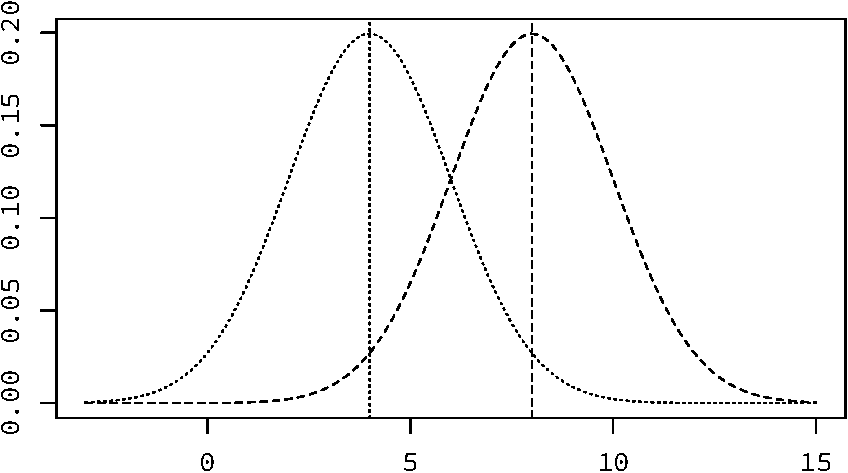
\includegraphics[width=0.9\linewidth,]{R_files/figure-latex/unnamed-chunk-86-1} \end{center}

 

\hypertarget{ux30c7ux30fcux30bfux306bux4e00ux5b9aux6570ux3092ux4e57ux3058ux305fux5834ux5408}{%
\subsection*{データに一定数を乗じた場合}\label{ux30c7ux30fcux30bfux306bux4e00ux5b9aux6570ux3092ux4e57ux3058ux305fux5834ux5408}}
\addcontentsline{toc}{subsection}{データに一定数を乗じた場合}

 それぞれに\(2\)を乗ずる。

\begin{Shaded}
\begin{Highlighting}[]
\NormalTok{x }\SpecialCharTok{\%\textgreater{}\%} 
\NormalTok{  dplyr}\SpecialCharTok{::}\FunctionTok{mutate}\NormalTok{(}\AttributeTok{Y =}\NormalTok{ X }\SpecialCharTok{*} \DecValTok{2}\NormalTok{)}
\end{Highlighting}
\end{Shaded}

\begin{verbatim}
##   X  Y
## 1 1  2
## 2 3  6
## 3 4  8
## 4 5 10
## 5 7 14
\end{verbatim}

\begin{Shaded}
\begin{Highlighting}[]
\NormalTok{mean }\OtherTok{\textless{}{-}}\NormalTok{ x }\SpecialCharTok{\%\textgreater{}\%} 
\NormalTok{  dplyr}\SpecialCharTok{::}\FunctionTok{mutate}\NormalTok{(}\AttributeTok{Y =}\NormalTok{ X }\SpecialCharTok{*} \DecValTok{2}\NormalTok{) }\SpecialCharTok{\%\textgreater{}\%} 
\NormalTok{  dplyr}\SpecialCharTok{::}\FunctionTok{summarise}\NormalTok{(}\AttributeTok{X =} \FunctionTok{mean}\NormalTok{(X), }\AttributeTok{Y =} \FunctionTok{mean}\NormalTok{(Y))}
\NormalTok{mean}
\end{Highlighting}
\end{Shaded}

\begin{verbatim}
##   X Y
## 1 4 8
\end{verbatim}

 偏差

\begin{Shaded}
\begin{Highlighting}[]
\NormalTok{dev }\OtherTok{\textless{}{-}}\NormalTok{ x }\SpecialCharTok{\%\textgreater{}\%} 
\NormalTok{  dplyr}\SpecialCharTok{::}\FunctionTok{mutate}\NormalTok{(}\AttributeTok{Y =}\NormalTok{ X }\SpecialCharTok{*} \DecValTok{2}\NormalTok{) }\SpecialCharTok{\%\textgreater{}\%} 
\NormalTok{  dplyr}\SpecialCharTok{::}\FunctionTok{mutate}\NormalTok{(}\AttributeTok{X =}\NormalTok{ X }\SpecialCharTok{{-}}\NormalTok{ mean}\SpecialCharTok{$}\NormalTok{X, }\AttributeTok{Y =}\NormalTok{ Y }\SpecialCharTok{{-}}\NormalTok{ mean}\SpecialCharTok{$}\NormalTok{Y)}
\NormalTok{dev}
\end{Highlighting}
\end{Shaded}

\begin{verbatim}
##    X  Y
## 1 -3 -6
## 2 -1 -2
## 3  0  0
## 4  1  2
## 5  3  6
\end{verbatim}

 分散

\begin{Shaded}
\begin{Highlighting}[]
\NormalTok{var }\OtherTok{\textless{}{-}}\NormalTok{ dev }\SpecialCharTok{\%\textgreater{}\%} 
\NormalTok{  dplyr}\SpecialCharTok{::}\FunctionTok{summarize}\NormalTok{(}\AttributeTok{X =} \FunctionTok{sum}\NormalTok{(X }\SpecialCharTok{\^{}} \DecValTok{2}\NormalTok{) }\SpecialCharTok{/} \FunctionTok{length}\NormalTok{(X), }\AttributeTok{Y =} \FunctionTok{sum}\NormalTok{(Y }\SpecialCharTok{\^{}} \DecValTok{2}\NormalTok{) }\SpecialCharTok{/} \FunctionTok{length}\NormalTok{(Y))}
\NormalTok{var}
\end{Highlighting}
\end{Shaded}

\begin{verbatim}
##   X  Y
## 1 4 16
\end{verbatim}

 標準偏差

\begin{Shaded}
\begin{Highlighting}[]
\FunctionTok{sqrt}\NormalTok{(var)}
\end{Highlighting}
\end{Shaded}

\begin{verbatim}
##   X Y
## 1 2 4
\end{verbatim}

 以上のようにデータに一定数を乗じると平均値は乗じた一定値の分だけ大きくなり、他の統計量も乗じた一定値の分だけ大きくなっていることが分かります。これを正規分布で図示すると下図のようになります。

\begin{Shaded}
\begin{Highlighting}[]
\FunctionTok{curve}\NormalTok{(}\FunctionTok{dnorm}\NormalTok{(x, }\AttributeTok{mean =} \DecValTok{4}\NormalTok{, }\AttributeTok{sd =} \DecValTok{2}\NormalTok{), }\SpecialCharTok{{-}}\DecValTok{3}\NormalTok{, }\DecValTok{15}\NormalTok{, }\AttributeTok{lty =} \DecValTok{3}\NormalTok{, }\AttributeTok{xlab =} \StringTok{""}\NormalTok{, }\AttributeTok{ylab =} \StringTok{""}\NormalTok{)}
\FunctionTok{abline}\NormalTok{(}\AttributeTok{v =} \DecValTok{4}\NormalTok{, }\AttributeTok{lty =} \DecValTok{3}\NormalTok{)}
\FunctionTok{curve}\NormalTok{(}\FunctionTok{dnorm}\NormalTok{(x, }\AttributeTok{mean =} \DecValTok{8}\NormalTok{, }\AttributeTok{sd =} \DecValTok{4}\NormalTok{), }\SpecialCharTok{{-}}\DecValTok{3}\NormalTok{, }\DecValTok{15}\NormalTok{, }\AttributeTok{add =} \ConstantTok{TRUE}\NormalTok{, }\AttributeTok{lty =} \DecValTok{2}\NormalTok{,}
      \AttributeTok{xlab =} \StringTok{""}\NormalTok{, }\AttributeTok{ylab =} \StringTok{""}\NormalTok{)}
\FunctionTok{abline}\NormalTok{(}\AttributeTok{v =} \DecValTok{8}\NormalTok{, }\AttributeTok{lty =} \DecValTok{2}\NormalTok{)}
\end{Highlighting}
\end{Shaded}

\begin{center}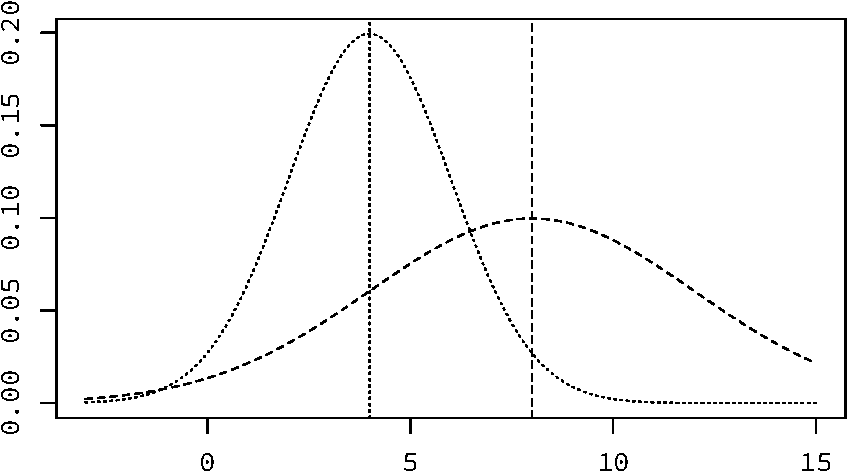
\includegraphics[width=0.9\linewidth,]{R_files/figure-latex/unnamed-chunk-92-1} \end{center}

 

\begin{longtable}[]{@{}
  >{\raggedright\arraybackslash}p{(\columnwidth - 6\tabcolsep) * \real{0.3205}}
  >{\centering\arraybackslash}p{(\columnwidth - 6\tabcolsep) * \real{0.2564}}
  >{\centering\arraybackslash}p{(\columnwidth - 6\tabcolsep) * \real{0.1923}}
  >{\raggedright\arraybackslash}p{(\columnwidth - 6\tabcolsep) * \real{0.2308}}@{}}
\toprule
\begin{minipage}[b]{\linewidth}\raggedright
加工方法
\end{minipage} & \begin{minipage}[b]{\linewidth}\centering
平均値
\end{minipage} & \begin{minipage}[b]{\linewidth}\centering
標準偏差
\end{minipage} & \begin{minipage}[b]{\linewidth}\raggedright
備考
\end{minipage} \\
\midrule
\endhead
無加工(元データ\(x\)) & \(\bar{x}\) & \(SD\) & \\
定数の加算(\(x + k\)) & \(\bar{x} + k\) & \(SD\) & 変化するのは平均値のみ \\
定数の乗算(\(x \times k\)) & \(\bar{x} \times k\) & \(SD \times k\) & 平均値・標準偏差ともに変化 \\
\bottomrule
\end{longtable}

\(k\): 任意の実数

 

\hypertarget{ux6a19ux6e96ux504fux5deeux4f55ux500bux5206ux3068ux306aux308bux3088ux3046ux306bux30c7ux30fcux30bfux3092ux52a0ux5de5ux3059ux308bux52b9ux679c}{%
\subsection*{標準偏差何個分となるようにデータを加工する効果}\label{ux6a19ux6e96ux504fux5deeux4f55ux500bux5206ux3068ux306aux308bux3088ux3046ux306bux30c7ux30fcux30bfux3092ux52a0ux5de5ux3059ux308bux52b9ux679c}}
\addcontentsline{toc}{subsection}{標準偏差何個分となるようにデータを加工する効果}

 ここで説明されているのは「正規化」です。

\begin{Shaded}
\begin{Highlighting}[]
\NormalTok{x }\OtherTok{\textless{}{-}} \FunctionTok{read.csv}\NormalTok{(}\AttributeTok{file =} \StringTok{"../data/P49\_図表4{-}5.csv"}\NormalTok{)}
\NormalTok{x}
\end{Highlighting}
\end{Shaded}

\begin{verbatim}
##   X
## 1 1
## 2 3
## 3 4
## 4 5
## 5 7
\end{verbatim}

 上記のP49のデータは、平均値\(4\)、標準偏差\(2\)ですので、\((データ - 平均値) \div 標準偏差\)を計算すると下記のようになります。

\begin{Shaded}
\begin{Highlighting}[]
\NormalTok{x }\SpecialCharTok{\%\textgreater{}\%} 
\NormalTok{  dplyr}\SpecialCharTok{::}\FunctionTok{mutate}\NormalTok{(}\AttributeTok{dev =}\NormalTok{ (X }\SpecialCharTok{{-}}\NormalTok{ (}\FunctionTok{sum}\NormalTok{(X) }\SpecialCharTok{/} \FunctionTok{length}\NormalTok{(X))),            }\CommentTok{\# 偏差}
                \AttributeTok{nX =}\NormalTok{ dev }\SpecialCharTok{/} \FunctionTok{sqrt}\NormalTok{(}\FunctionTok{sum}\NormalTok{(dev }\SpecialCharTok{\^{}} \DecValTok{2}\NormalTok{) }\SpecialCharTok{/} \FunctionTok{length}\NormalTok{(dev))) }\CommentTok{\# 正規化値}
\end{Highlighting}
\end{Shaded}

\begin{verbatim}
##   X dev   nX
## 1 1  -3 -1.5
## 2 3  -1 -0.5
## 3 4   0  0.0
## 4 5   1  0.5
## 5 7   3  1.5
\end{verbatim}

 \texttt{nX}の平均値と標準偏差は以下のように\(0\)と\(1\)になることが分かります。

\begin{Shaded}
\begin{Highlighting}[]
\NormalTok{x }\SpecialCharTok{\%\textgreater{}\%} 
\NormalTok{  dplyr}\SpecialCharTok{::}\FunctionTok{mutate}\NormalTok{(}\AttributeTok{nX =}\NormalTok{ (X }\SpecialCharTok{{-}} \DecValTok{4}\NormalTok{) }\SpecialCharTok{/} \DecValTok{2}\NormalTok{) }\SpecialCharTok{\%\textgreater{}\%} 
\NormalTok{  dplyr}\SpecialCharTok{::}\FunctionTok{summarise}\NormalTok{(}\AttributeTok{mean =} \FunctionTok{sum}\NormalTok{(nX) }\SpecialCharTok{/} \FunctionTok{length}\NormalTok{(nX),}
                   \AttributeTok{sd =} \FunctionTok{sqrt}\NormalTok{(}\FunctionTok{sum}\NormalTok{((nX }\SpecialCharTok{{-}}\NormalTok{ mean) }\SpecialCharTok{\^{}} \DecValTok{2}\NormalTok{) }\SpecialCharTok{/} \FunctionTok{length}\NormalTok{(nX)))}
\end{Highlighting}
\end{Shaded}

\begin{verbatim}
##   mean sd
## 1    0  1
\end{verbatim}

\hypertarget{ux7df4ux7fd2ux554fux984c-3}{%
\section*{練習問題}\label{ux7df4ux7fd2ux554fux984c-3}}
\addcontentsline{toc}{section}{練習問題}

 (省略)

 

\hypertarget{ux30b3ux30e9ux30e0ux504fux5deeux5024ux3067ux5accux306aux601dux3044ux3092ux3057ux305fux3053ux3068ux306eux3042ux308bux3042ux306aux305fux306b}{%
\section*{【コラム】偏差値で嫌な思いをしたことのあるあなたに}\label{ux30b3ux30e9ux30e0ux504fux5deeux5024ux3067ux5accux306aux601dux3044ux3092ux3057ux305fux3053ux3068ux306eux3042ux308bux3042ux306aux305fux306b}}
\addcontentsline{toc}{section}{【コラム】偏差値で嫌な思いをしたことのあるあなたに}

 

\hypertarget{ux8ffdux52a0ux554fux984c-2}{%
\section*{追加問題}\label{ux8ffdux52a0ux554fux984c-2}}
\addcontentsline{toc}{section}{追加問題}

 P16の身長データを正規化(\((\mbox{データ} - \mbox{平均値}) \div \mbox{標準偏差}\))してみましょう。

\hypertarget{ux89e3ux7b54ux4f8b-4}{%
\subsection*{解答例}\label{ux89e3ux7b54ux4f8b-4}}
\addcontentsline{toc}{subsection}{解答例}

\begin{Shaded}
\begin{Highlighting}[]
\NormalTok{x }\OtherTok{\textless{}{-}} \StringTok{"../data/P16\_図表1{-}1 .csv"} \SpecialCharTok{\%\textgreater{}\%} 
\NormalTok{  readr}\SpecialCharTok{::}\FunctionTok{read\_csv}\NormalTok{(}\AttributeTok{col\_names =} \ConstantTok{FALSE}\NormalTok{, }\AttributeTok{show\_col\_types =} \ConstantTok{FALSE}\NormalTok{) }\SpecialCharTok{\%\textgreater{}\%} 
\NormalTok{  tidyr}\SpecialCharTok{::}\FunctionTok{pivot\_longer}\NormalTok{(}\AttributeTok{cols =}\NormalTok{ dplyr}\SpecialCharTok{::}\FunctionTok{starts\_with}\NormalTok{(}\StringTok{"X"}\NormalTok{),}
                      \AttributeTok{names\_to =} \StringTok{"name"}\NormalTok{, }\AttributeTok{values\_to =} \StringTok{"value"}\NormalTok{) }\SpecialCharTok{\%\textgreater{}\%} 
\NormalTok{  dplyr}\SpecialCharTok{::}\FunctionTok{arrange}\NormalTok{(name) }\SpecialCharTok{\%\textgreater{}\%} 
\NormalTok{  dplyr}\SpecialCharTok{::}\FunctionTok{select}\NormalTok{(}\AttributeTok{height =}\NormalTok{ value) }\SpecialCharTok{\%\textgreater{}\%} 
\NormalTok{  dplyr}\SpecialCharTok{::}\FunctionTok{mutate}\NormalTok{(}\AttributeTok{normalized =} \FunctionTok{scale}\NormalTok{(height))}
\NormalTok{x}
\end{Highlighting}
\end{Shaded}

\begin{verbatim}
## # A tibble: 80 x 2
##    height normalized[,1]
##     <dbl>          <dbl>
##  1    151        -1.22  
##  2    154        -0.661 
##  3    160         0.449 
##  4    160         0.449 
##  5    163         1.00  
##  6    156        -0.291 
##  7    158         0.0786
##  8    156        -0.291 
##  9    154        -0.661 
## 10    160         0.449 
## # ... with 70 more rows
\end{verbatim}

 正規化前後の平均値と標準偏差を比べると下記のようになります。

\begin{Shaded}
\begin{Highlighting}[]
\NormalTok{x }\SpecialCharTok{\%\textgreater{}\%} 
\NormalTok{  dplyr}\SpecialCharTok{::}\FunctionTok{summarise}\NormalTok{(}\AttributeTok{mean =} \FunctionTok{sum}\NormalTok{(height) }\SpecialCharTok{/} \FunctionTok{length}\NormalTok{(height),}
                   \AttributeTok{sd =} \FunctionTok{sqrt}\NormalTok{(}\FunctionTok{sum}\NormalTok{((height }\SpecialCharTok{{-}}\NormalTok{ mean)}\SpecialCharTok{\^{}} \DecValTok{2}\NormalTok{) }\SpecialCharTok{/} \FunctionTok{length}\NormalTok{(height)))}
\end{Highlighting}
\end{Shaded}

\begin{verbatim}
## # A tibble: 1 x 2
##    mean    sd
##   <dbl> <dbl>
## 1  158.  5.37
\end{verbatim}

\begin{Shaded}
\begin{Highlighting}[]
\NormalTok{x }\SpecialCharTok{\%\textgreater{}\%} 
\NormalTok{  dplyr}\SpecialCharTok{::}\FunctionTok{summarise}\NormalTok{(}\AttributeTok{mean =} \FunctionTok{sum}\NormalTok{(normalized) }\SpecialCharTok{/} \FunctionTok{length}\NormalTok{(normalized),}
                   \AttributeTok{sd =} \FunctionTok{sqrt}\NormalTok{(}\FunctionTok{sum}\NormalTok{((normalized }\SpecialCharTok{{-}}\NormalTok{ mean)}\SpecialCharTok{\^{}} \DecValTok{2}\NormalTok{) }\SpecialCharTok{/} \FunctionTok{length}\NormalTok{(normalized)))}
\end{Highlighting}
\end{Shaded}

\begin{verbatim}
## # A tibble: 1 x 2
##       mean    sd
##      <dbl> <dbl>
## 1 2.08e-15 0.994
\end{verbatim}

% --- Index(索引一覧)を作成する(ページがずれるバグあり)
% \cleardoublepage
% \phantomsection
% \printindex       % can be used to include the sorted and formatted index in the document.
% \see              % can used in the index to cross reference to other items.

% \cleardoublepage
% \phantomsection
% % \clearpage
% \vspace*{\stretch{1}}
% \begin{flushright}
% \begin{minipage}{0.5\hsize}
% \begin{description}
%   \item{著者:} Sampo Suzuki
%   % \item{表紙:} ASDF
%   \item{発行:} 2021年月日
%   % \item{サークル名:} ASDF
%   % \item{連絡先:} ASDF
%   % \item{印刷:} ASDF
% \end{description}
% \end{minipage}
% \end{flushright}
% \cleardoublepage
% % \clearpage

\end{document}
